\documentclass[conference]{IEEEtran}
\IEEEoverridecommandlockouts
% The preceding line is only needed to identify funding in the first footnote. If that is unneeded, please comment it out.
\usepackage{cite}
\usepackage{amsmath,amssymb,amsfonts}
\usepackage{algorithmic}
\usepackage{graphicx}
\usepackage{textcomp}
\usepackage{xcolor}
\def\BibTeX{{\rm B\kern-.05em{\sc i\kern-.025em b}\kern-.08em
    T\kern-.1667em\lower.7ex\hbox{E}\kern-.125emX}}
\begin{document}

\title{CENG 466 - Image Processing THE2 Report} \\

\author{
\IEEEauthorblockN{Muhammed Enes izgi}
\IEEEauthorblockA{\textit{Computer Engineering} \\
\textit{METU}\\
Ankara, Turkey \\
enes.izgi@metu.edu.tr}
\and
\IEEEauthorblockN{Emre Berk Kaya}
\IEEEauthorblockA{\textit{Computer Engineering} \\
\textit{METU}\\
Ankara, Turkey \\
emre.kaya\_03@metu.edu.tr}
}

\maketitle

\section{Introduction}
This document explains the methods used in second homework of Image Processing course.

\section{Face Detection}

Face detection can be done by using many techniques such as haar cascading or training deep learning model. Our face detection algorithm much more simpler than the other algorithms but it has some cons. \\

Our face detection algorithm works as follows: \\

1- First it applies gaussian blur to the image. We thought blurring the image makes our job easier while removing the background. \\

2- Second, we are applying a mask which we take as an argument to the function. This mask tries to remove the background. One of the cons of our algorithm is we need to give the skin color represented in the image. Otherwise, our algorithm cannot separate the faces from the background. Since, the images have very similar colors between faces and background, we need to find a mask and continue with other steps. \\

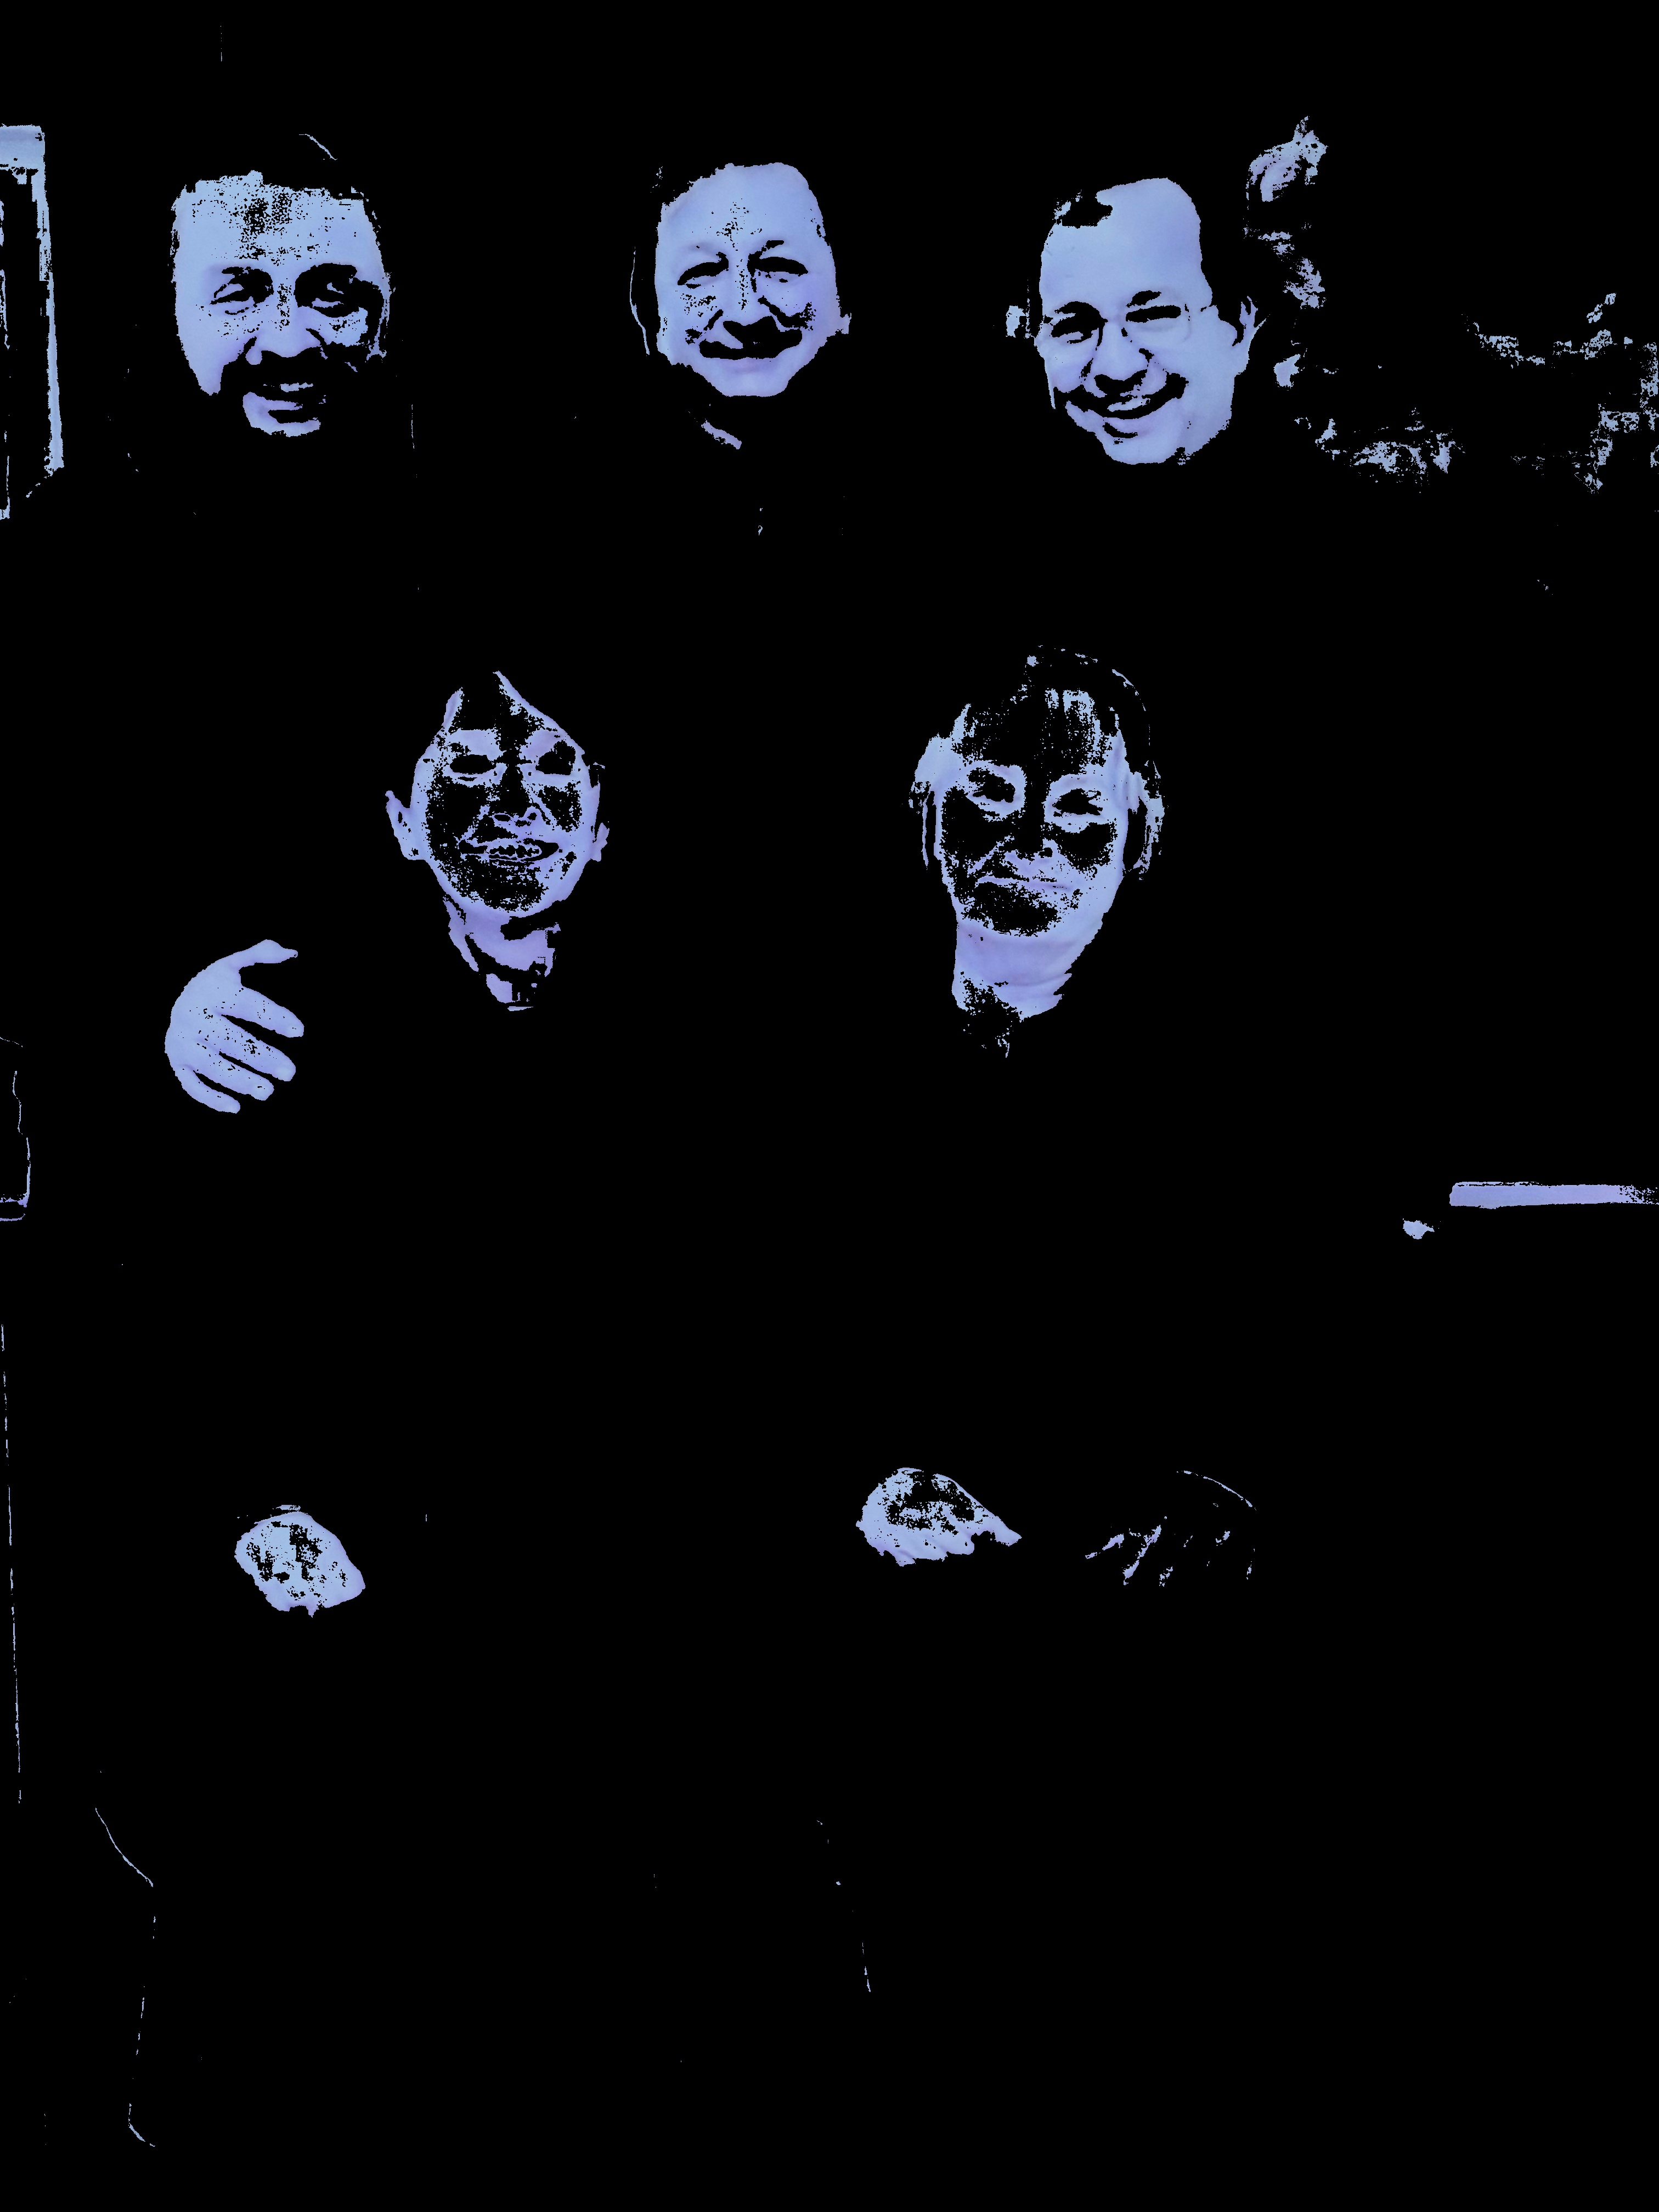
\includegraphics[scale=0.05]{mask.jpg}

3- Third, we need to get rid of the artifacts from the background. To remove these artifacts, we need to erode and dilate the image. After applying this step, if we used the correct skin color at step 2, algorithms works and find the faces. If it didn't work, we need to adjust our mask to find the faces. \\

Dilated image: \\

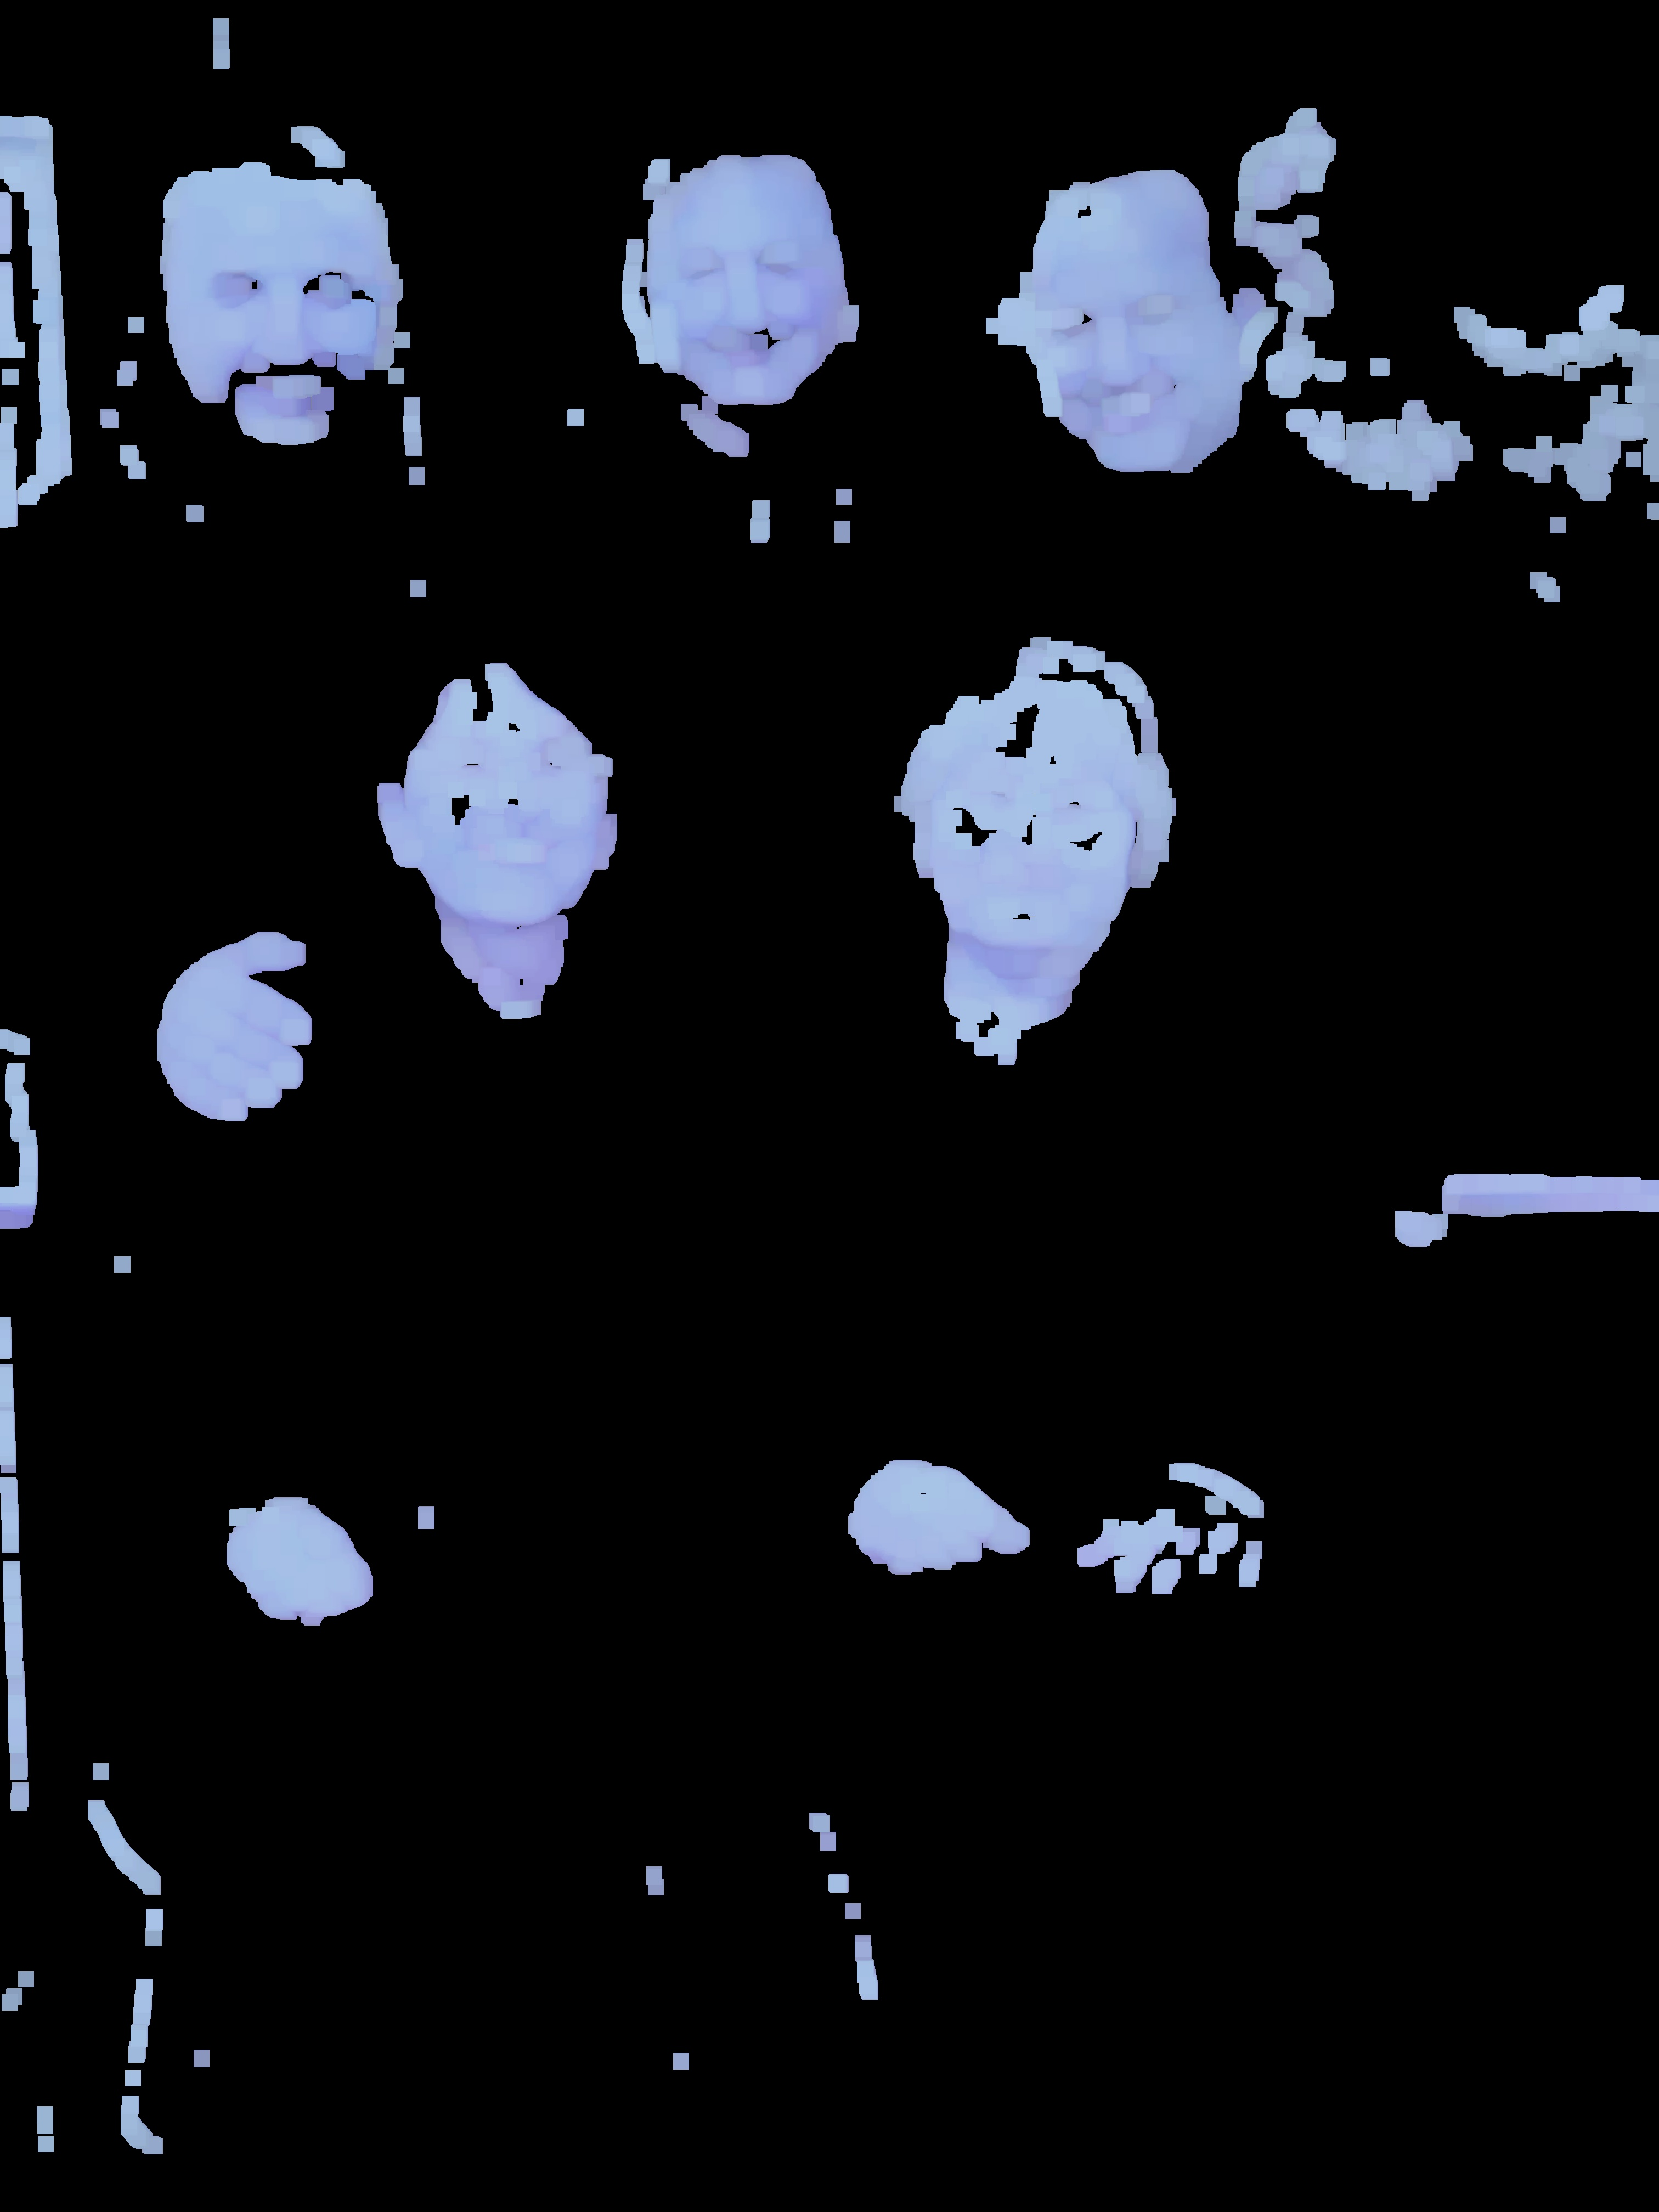
\includegraphics[scale=0.05]{dilation.jpg}

Eroded image: \\

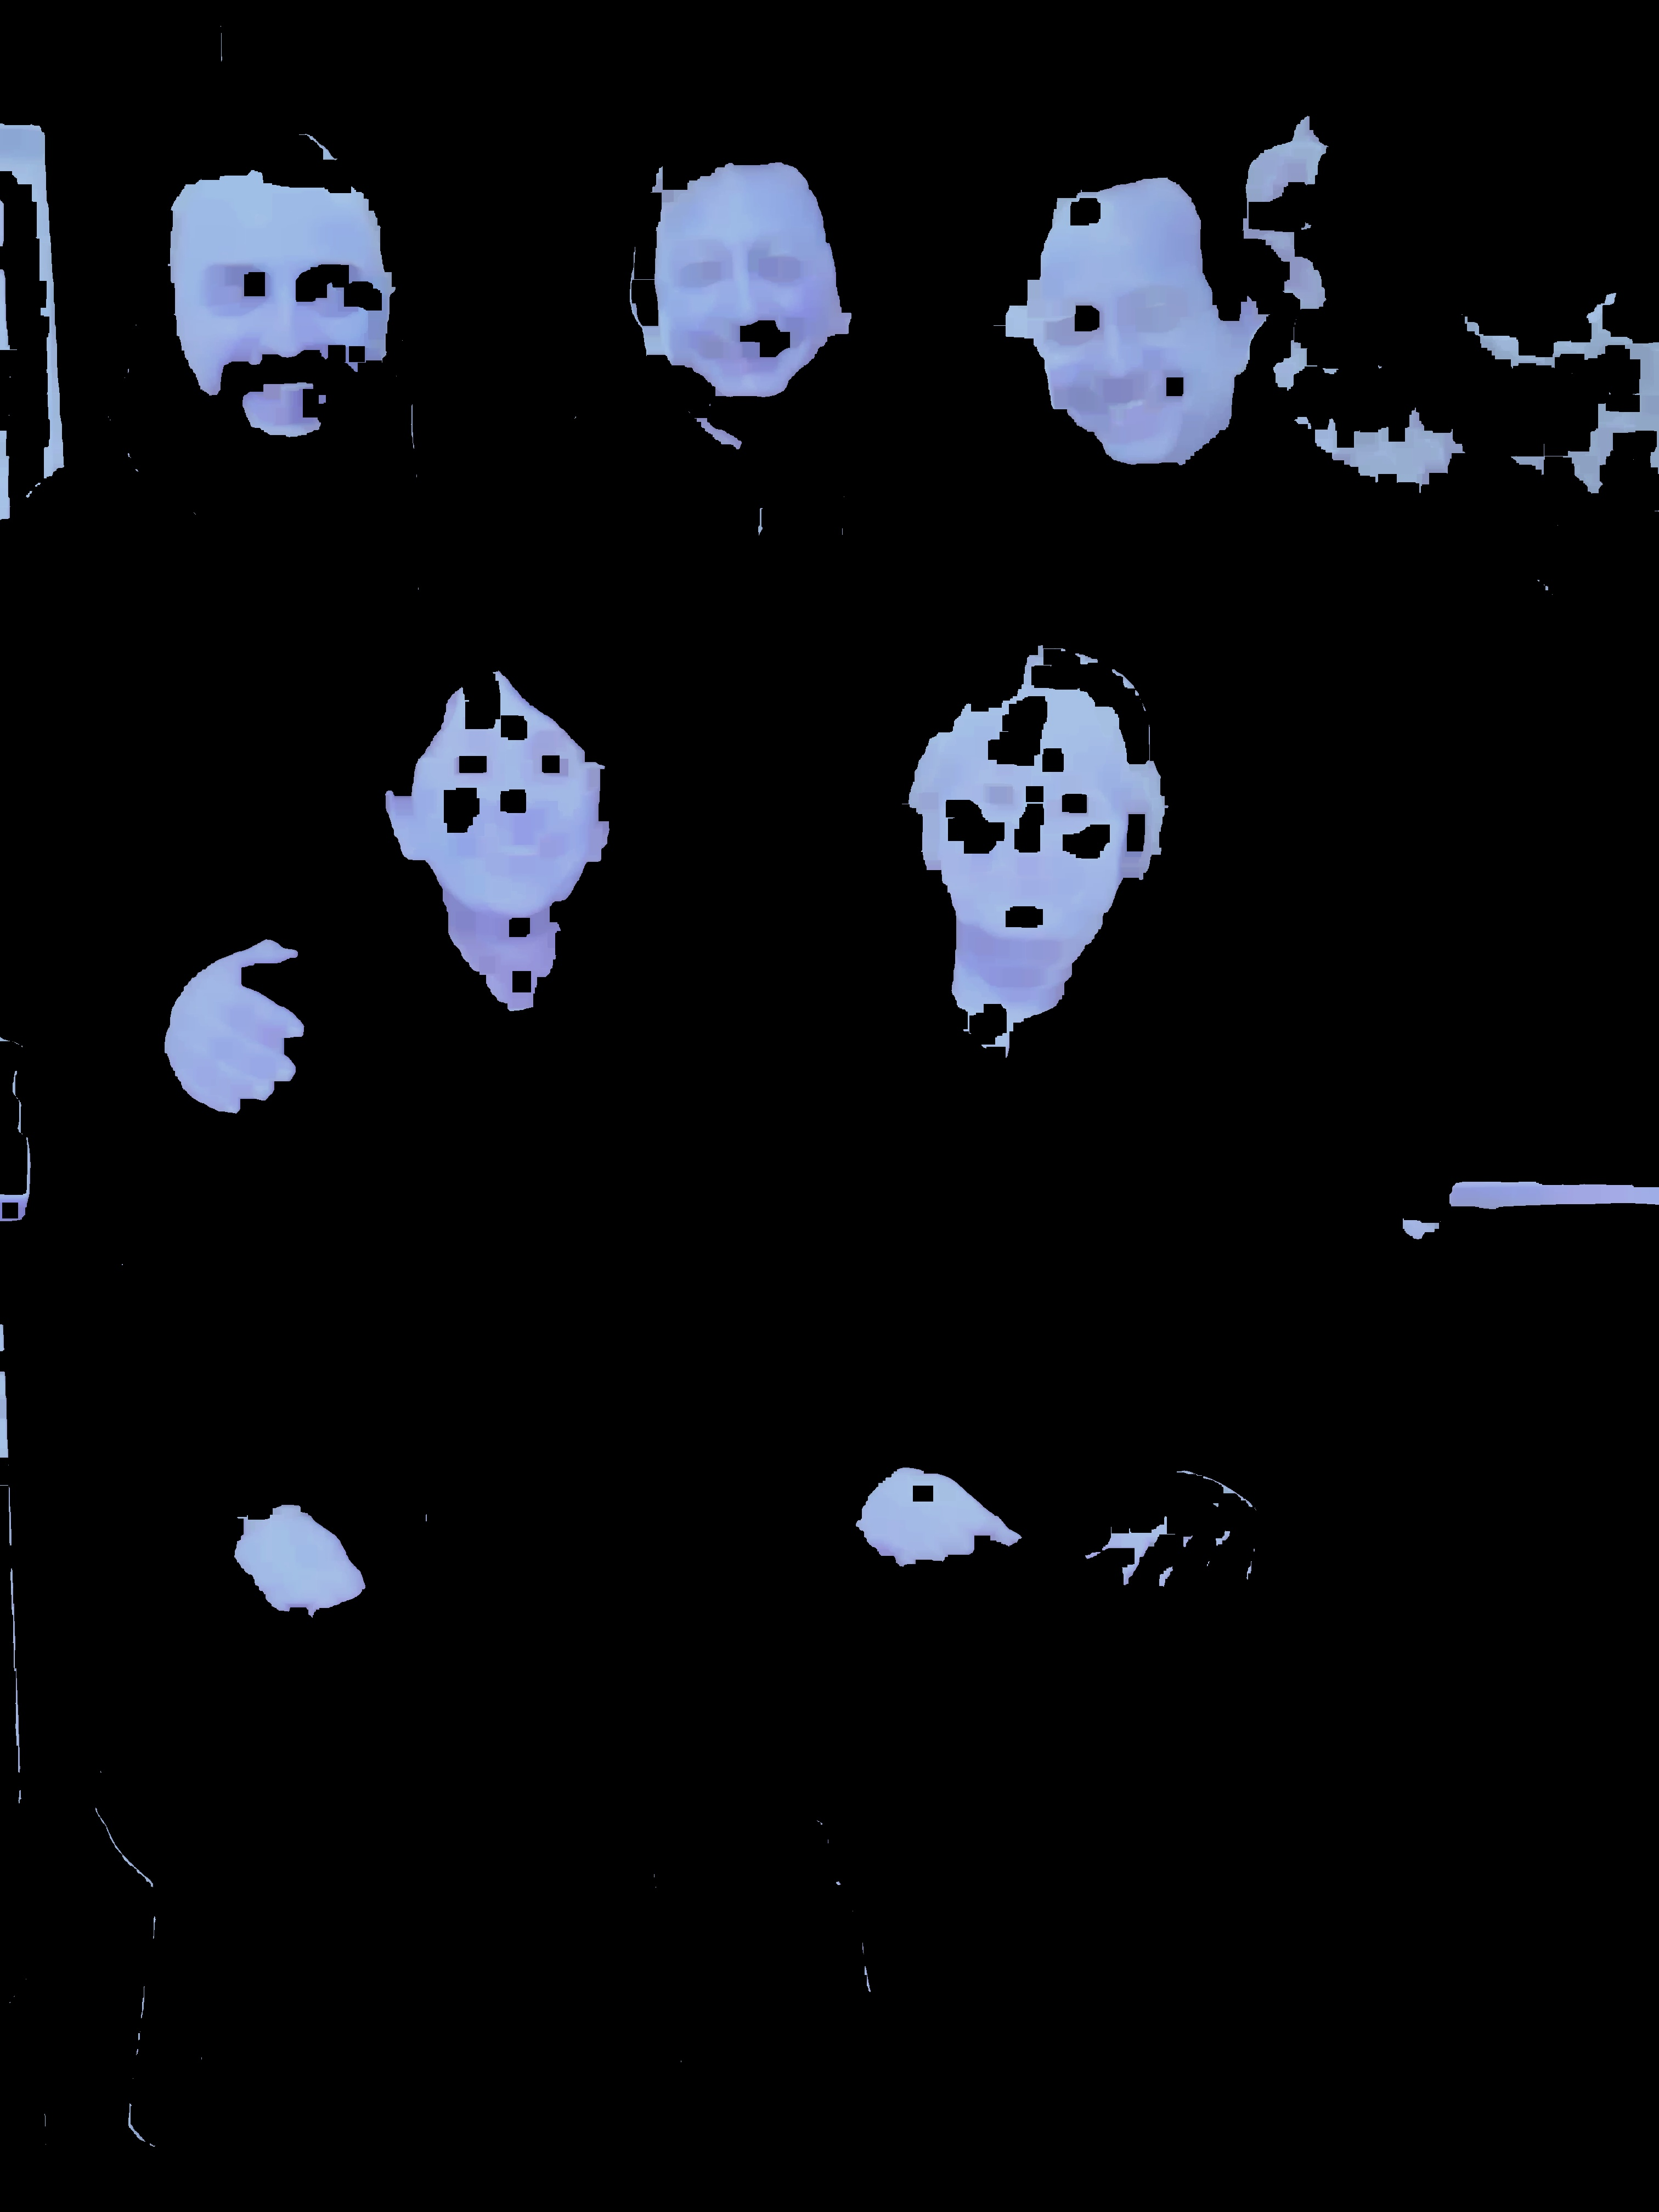
\includegraphics[scale=0.05]{erosion.jpg} \\

Also, we tried to to face detection with K-Means clustering. K-Means clustering gives us skin color in 1 cluster but we couldn't figure out which cluster to use for skin color. Maybe we can kluster the image and test the centers of clusters with a range value to see if cluster contains the faces. This approach would be better if we could choose the correct value by some method but we couldn't implement it correctly.

\section{Pseudo-coloring}
\subsection{Step 1}
Pseudo coloring is an image processing technique applied to gray scale images. For every gray level, we assign one color to that level. By applying this assignment, we obtain a colored image from a gray scale image. 
\subsection{Step 2}
Our algorithm runs as follows:
\begin{itemize}
\item Convert colored source image (name it source) to a grayscale image (name it source\_gray)
\item We will get {[r, g, b]} values for every pixel in source (source{[x]}{[y]}), and we will get {[grayLevel]} for every pixel in source\_gray.
\item Create an empty hash map (or dictionary, in Python), to map every gray level to {[r, g, b]} values (name it colorMap).
\item Loop through source and make assignment colorMap{[source\_gray{[x][y]}]} = source{[x][y]}
\item Create an image with zeros, that has same size with the image.
\item Loop through source\_gray and assign obtained {[r, g, b]} values to every pixel.
\item We get a colored image as a result.
\end{itemize}

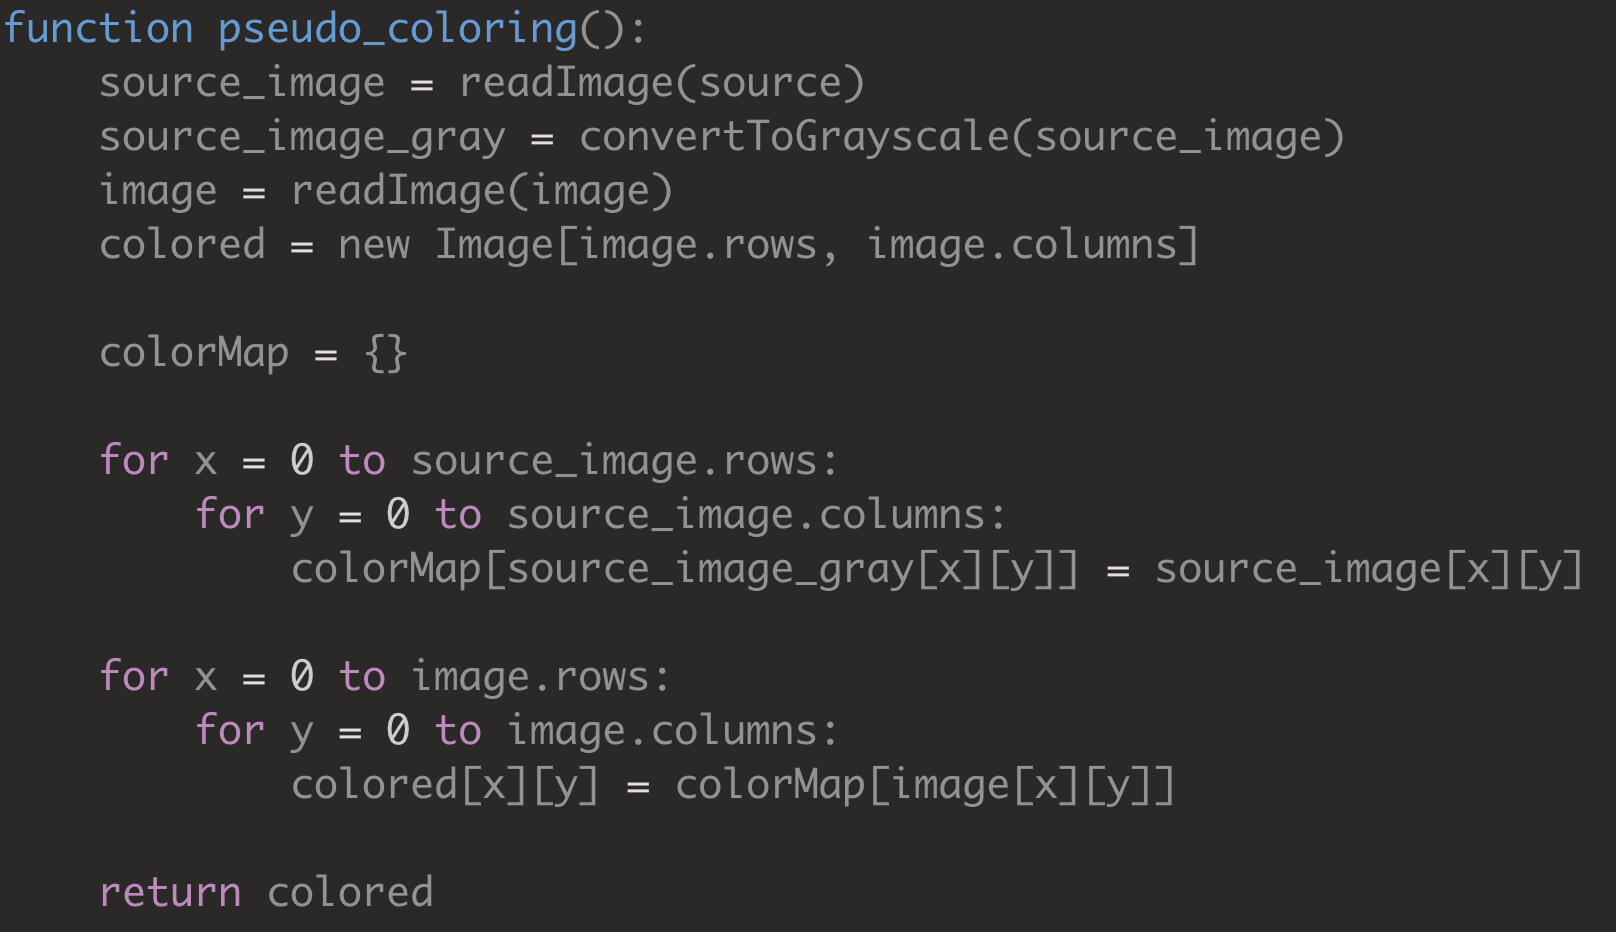
\includegraphics[width=\linewidth]{pseudocode.png}
\subsection{Step 3}
We obtained the following result, using this algorithm:
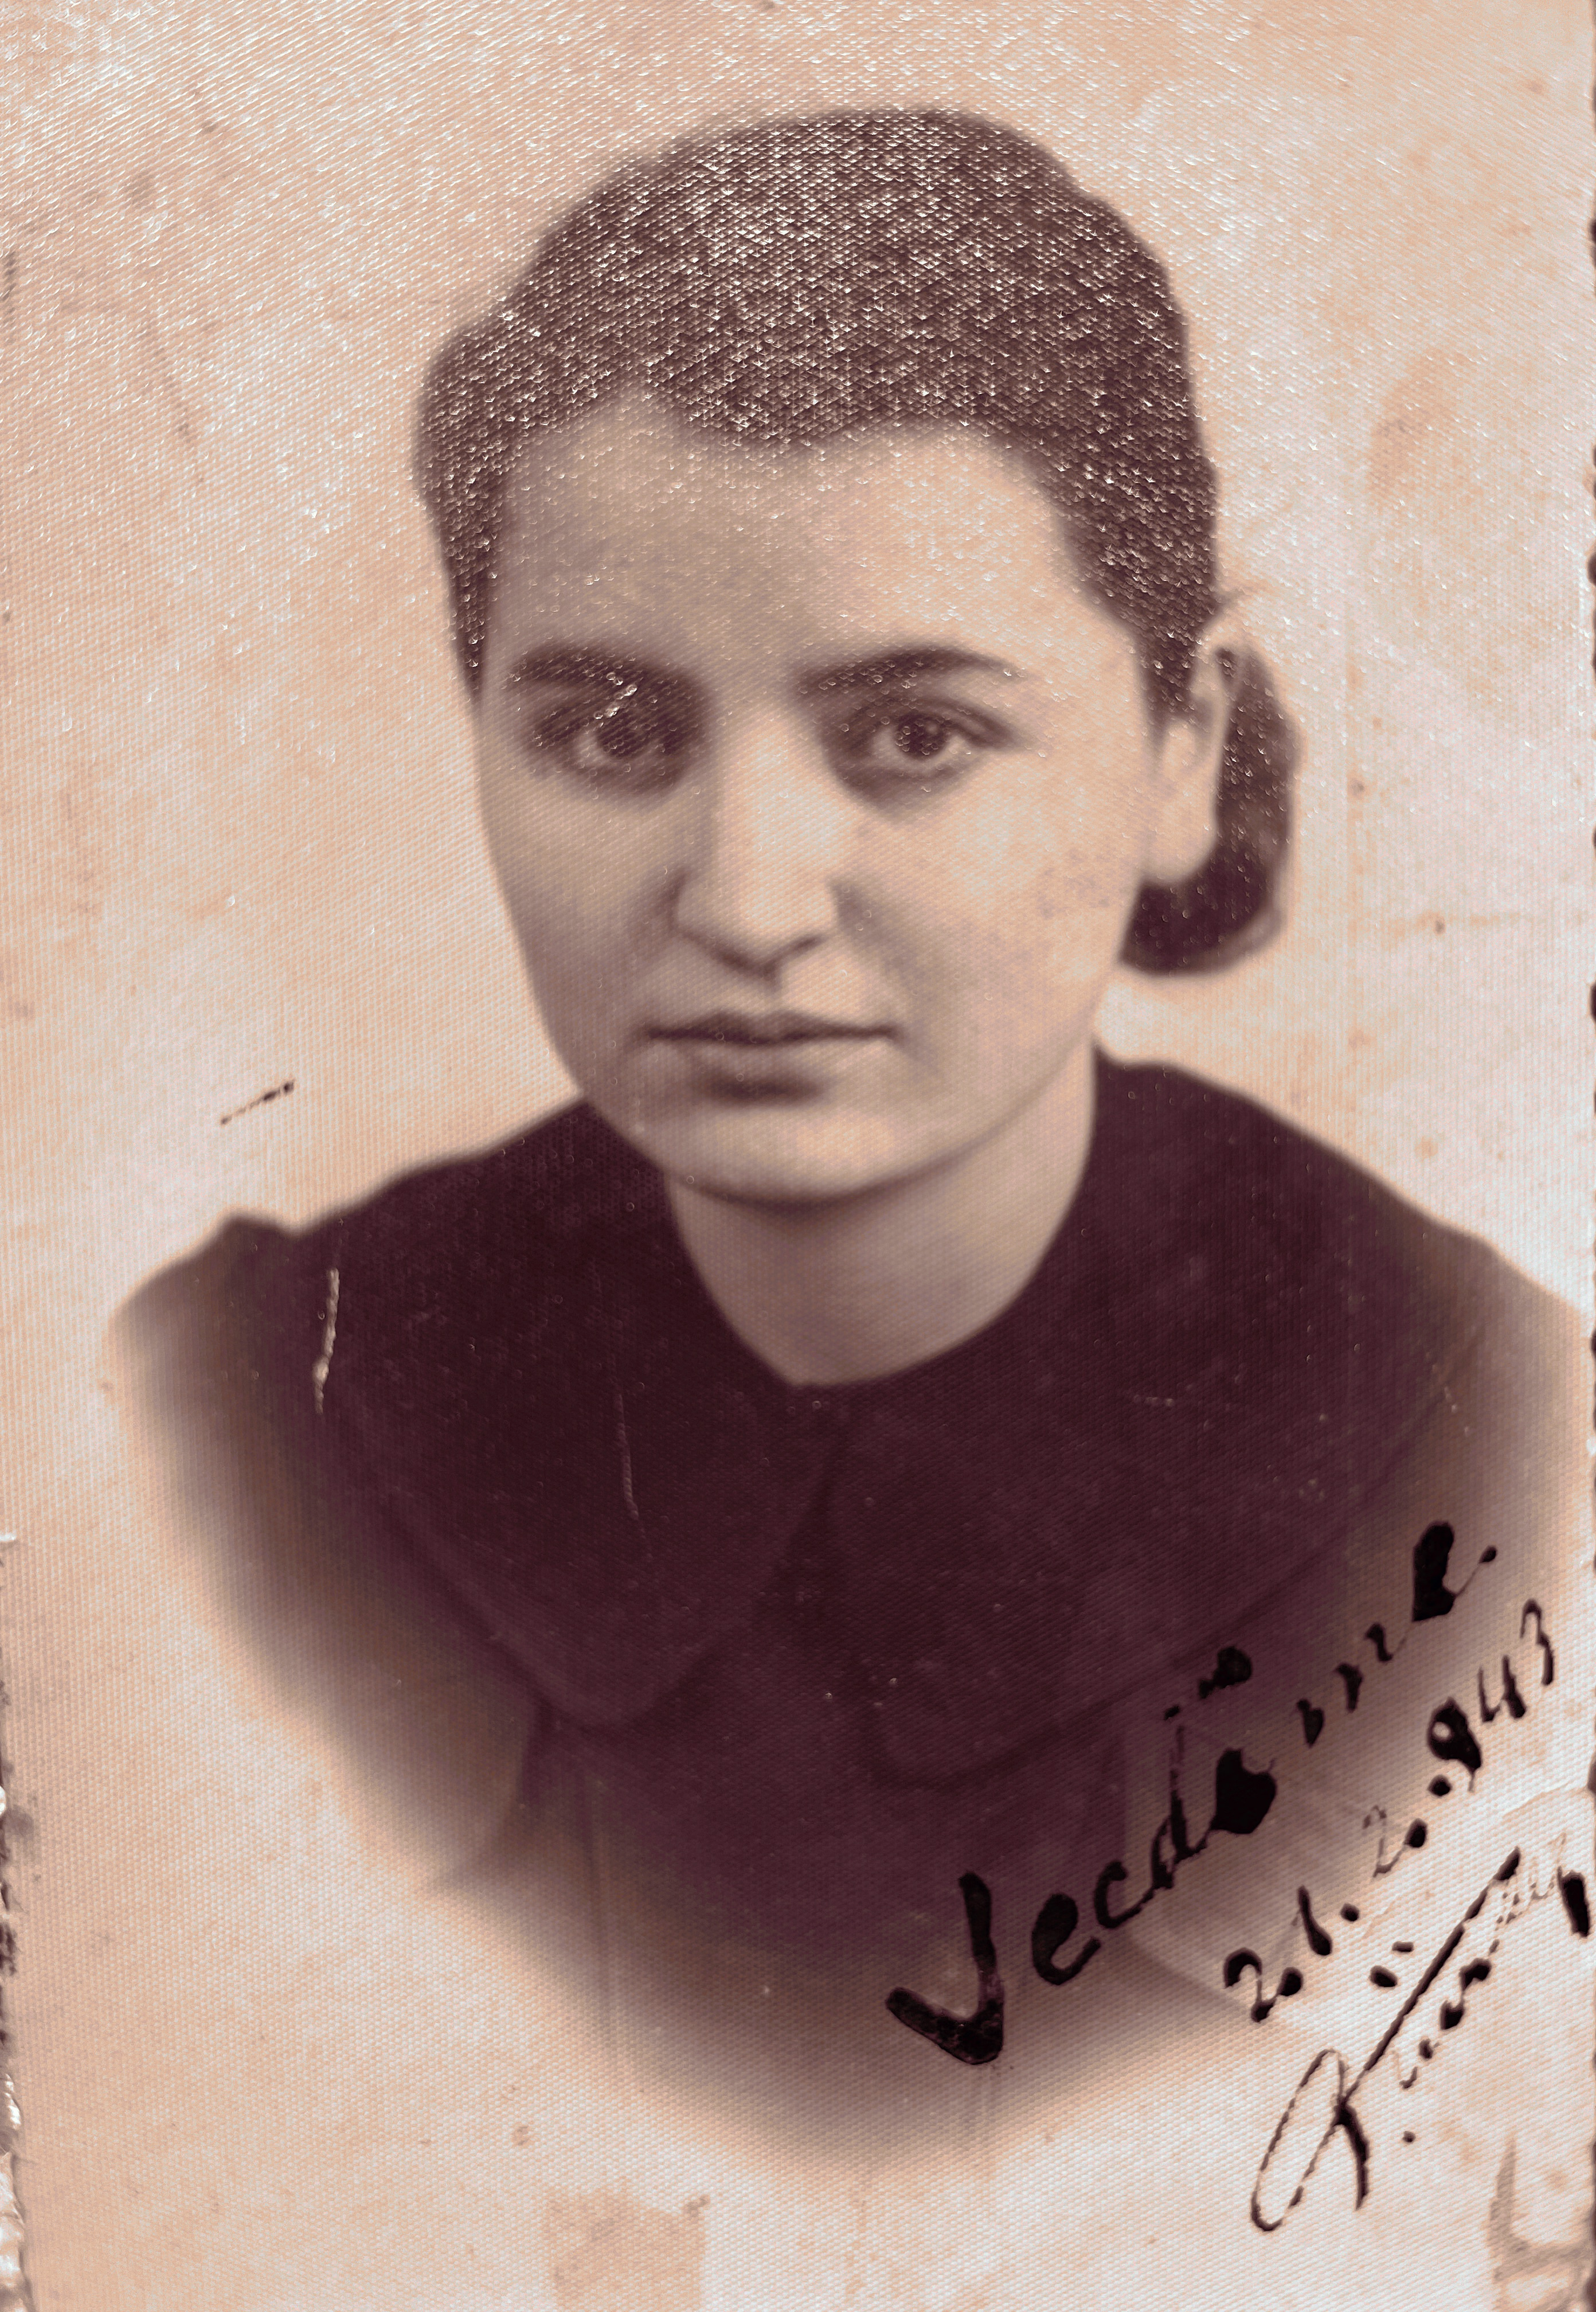
\includegraphics[width=0.5\linewidth]{3_colored.jpg}

Before running this algorithm, we tried to use another algorithm such that:
\begin{itemize}
        \item  Convert source image to HSI (or HSV) Image
        \item  Apply k-means to source and grayscale images with the same k value
        \item  We will get e.g. centers = [ [H=10, S=20, V=50], [20, 15, 30], [10, 10, 5] ] for source image
            We will get e.g. centers2 = [ [30], [20], [50], [100] ] for grayscale image
            Then sort them with their V values (keep a sortmap to remember the old places of centers2)
        \item  We will map H and S values of centers to centers2, regarding to their sorted indices.
        \item  We get centers2 = [ [H1, S1, V1], [H2, S2, V2], ... ]
        \item  Color the grayscale image with centers2 values. 
\end{itemize}
We obtained the following result, which is quite different than what we expected:

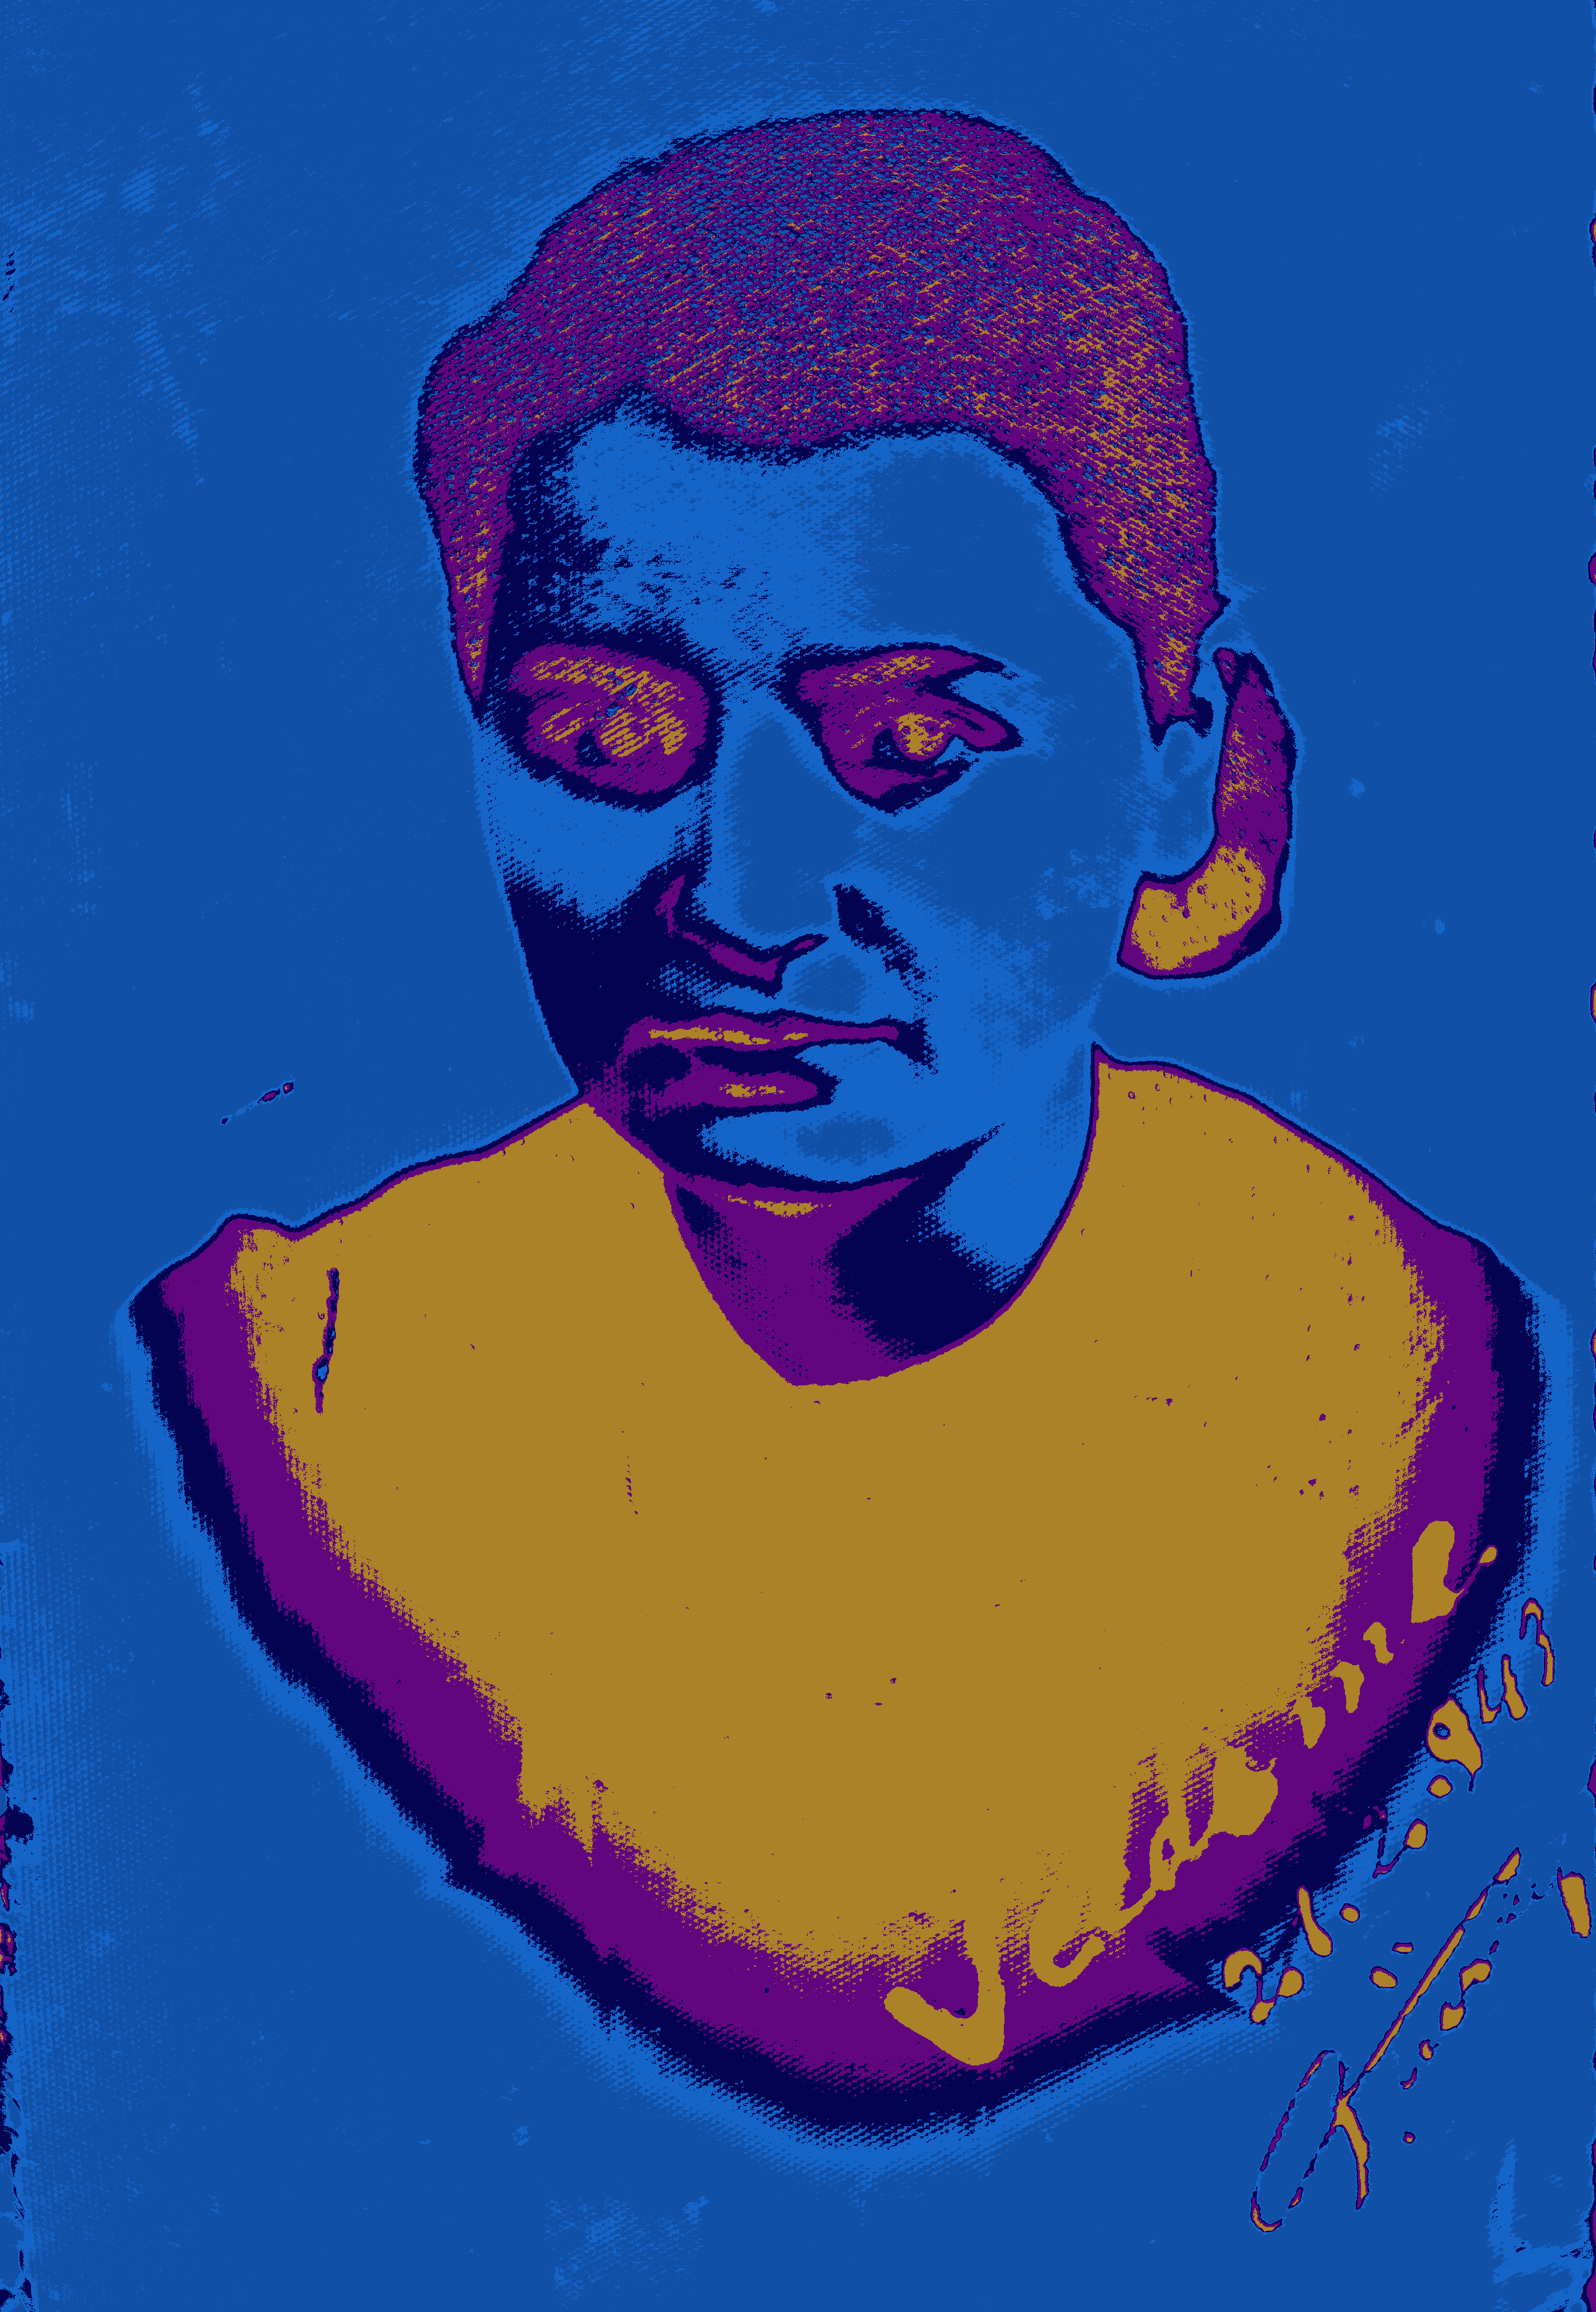
\includegraphics[width=0.5\linewidth]{test.png}

That's why, we included the first algorithm in our code.

\subsection{Step 5}
R, G, B channels as the result of pseudo-coloring for image 1: \\
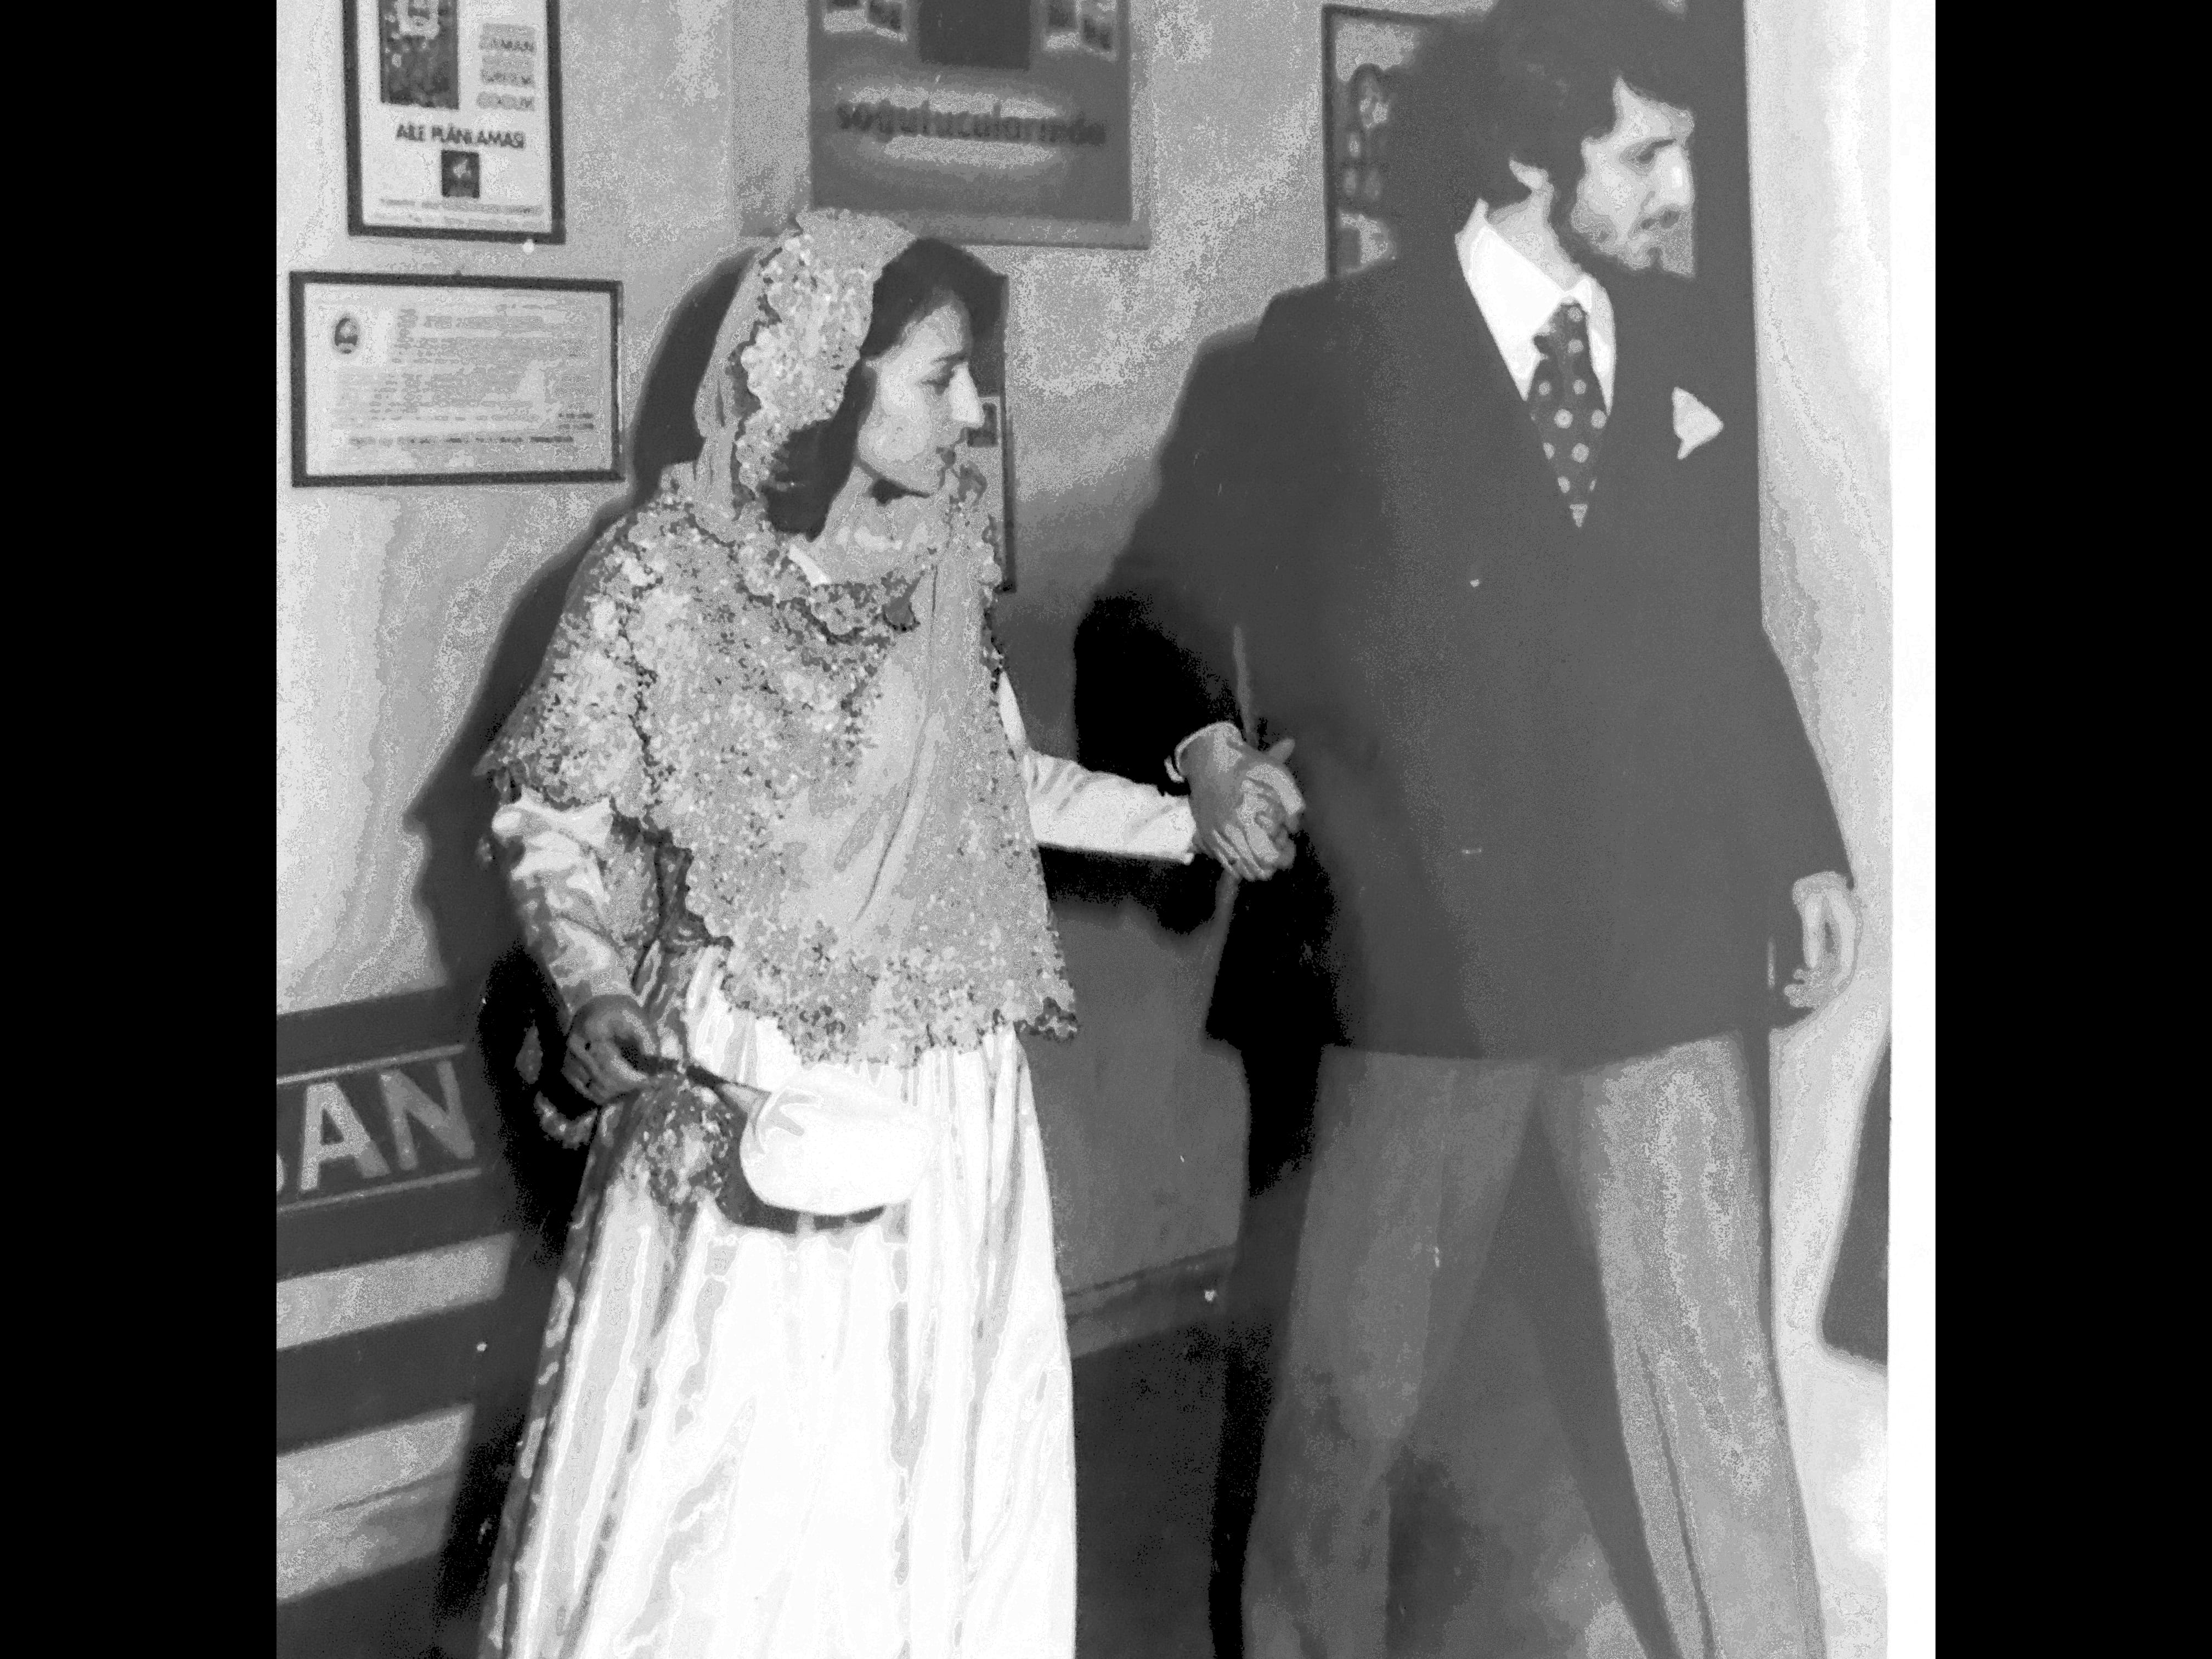
\includegraphics[width=0.3\linewidth]{1_R.jpg}
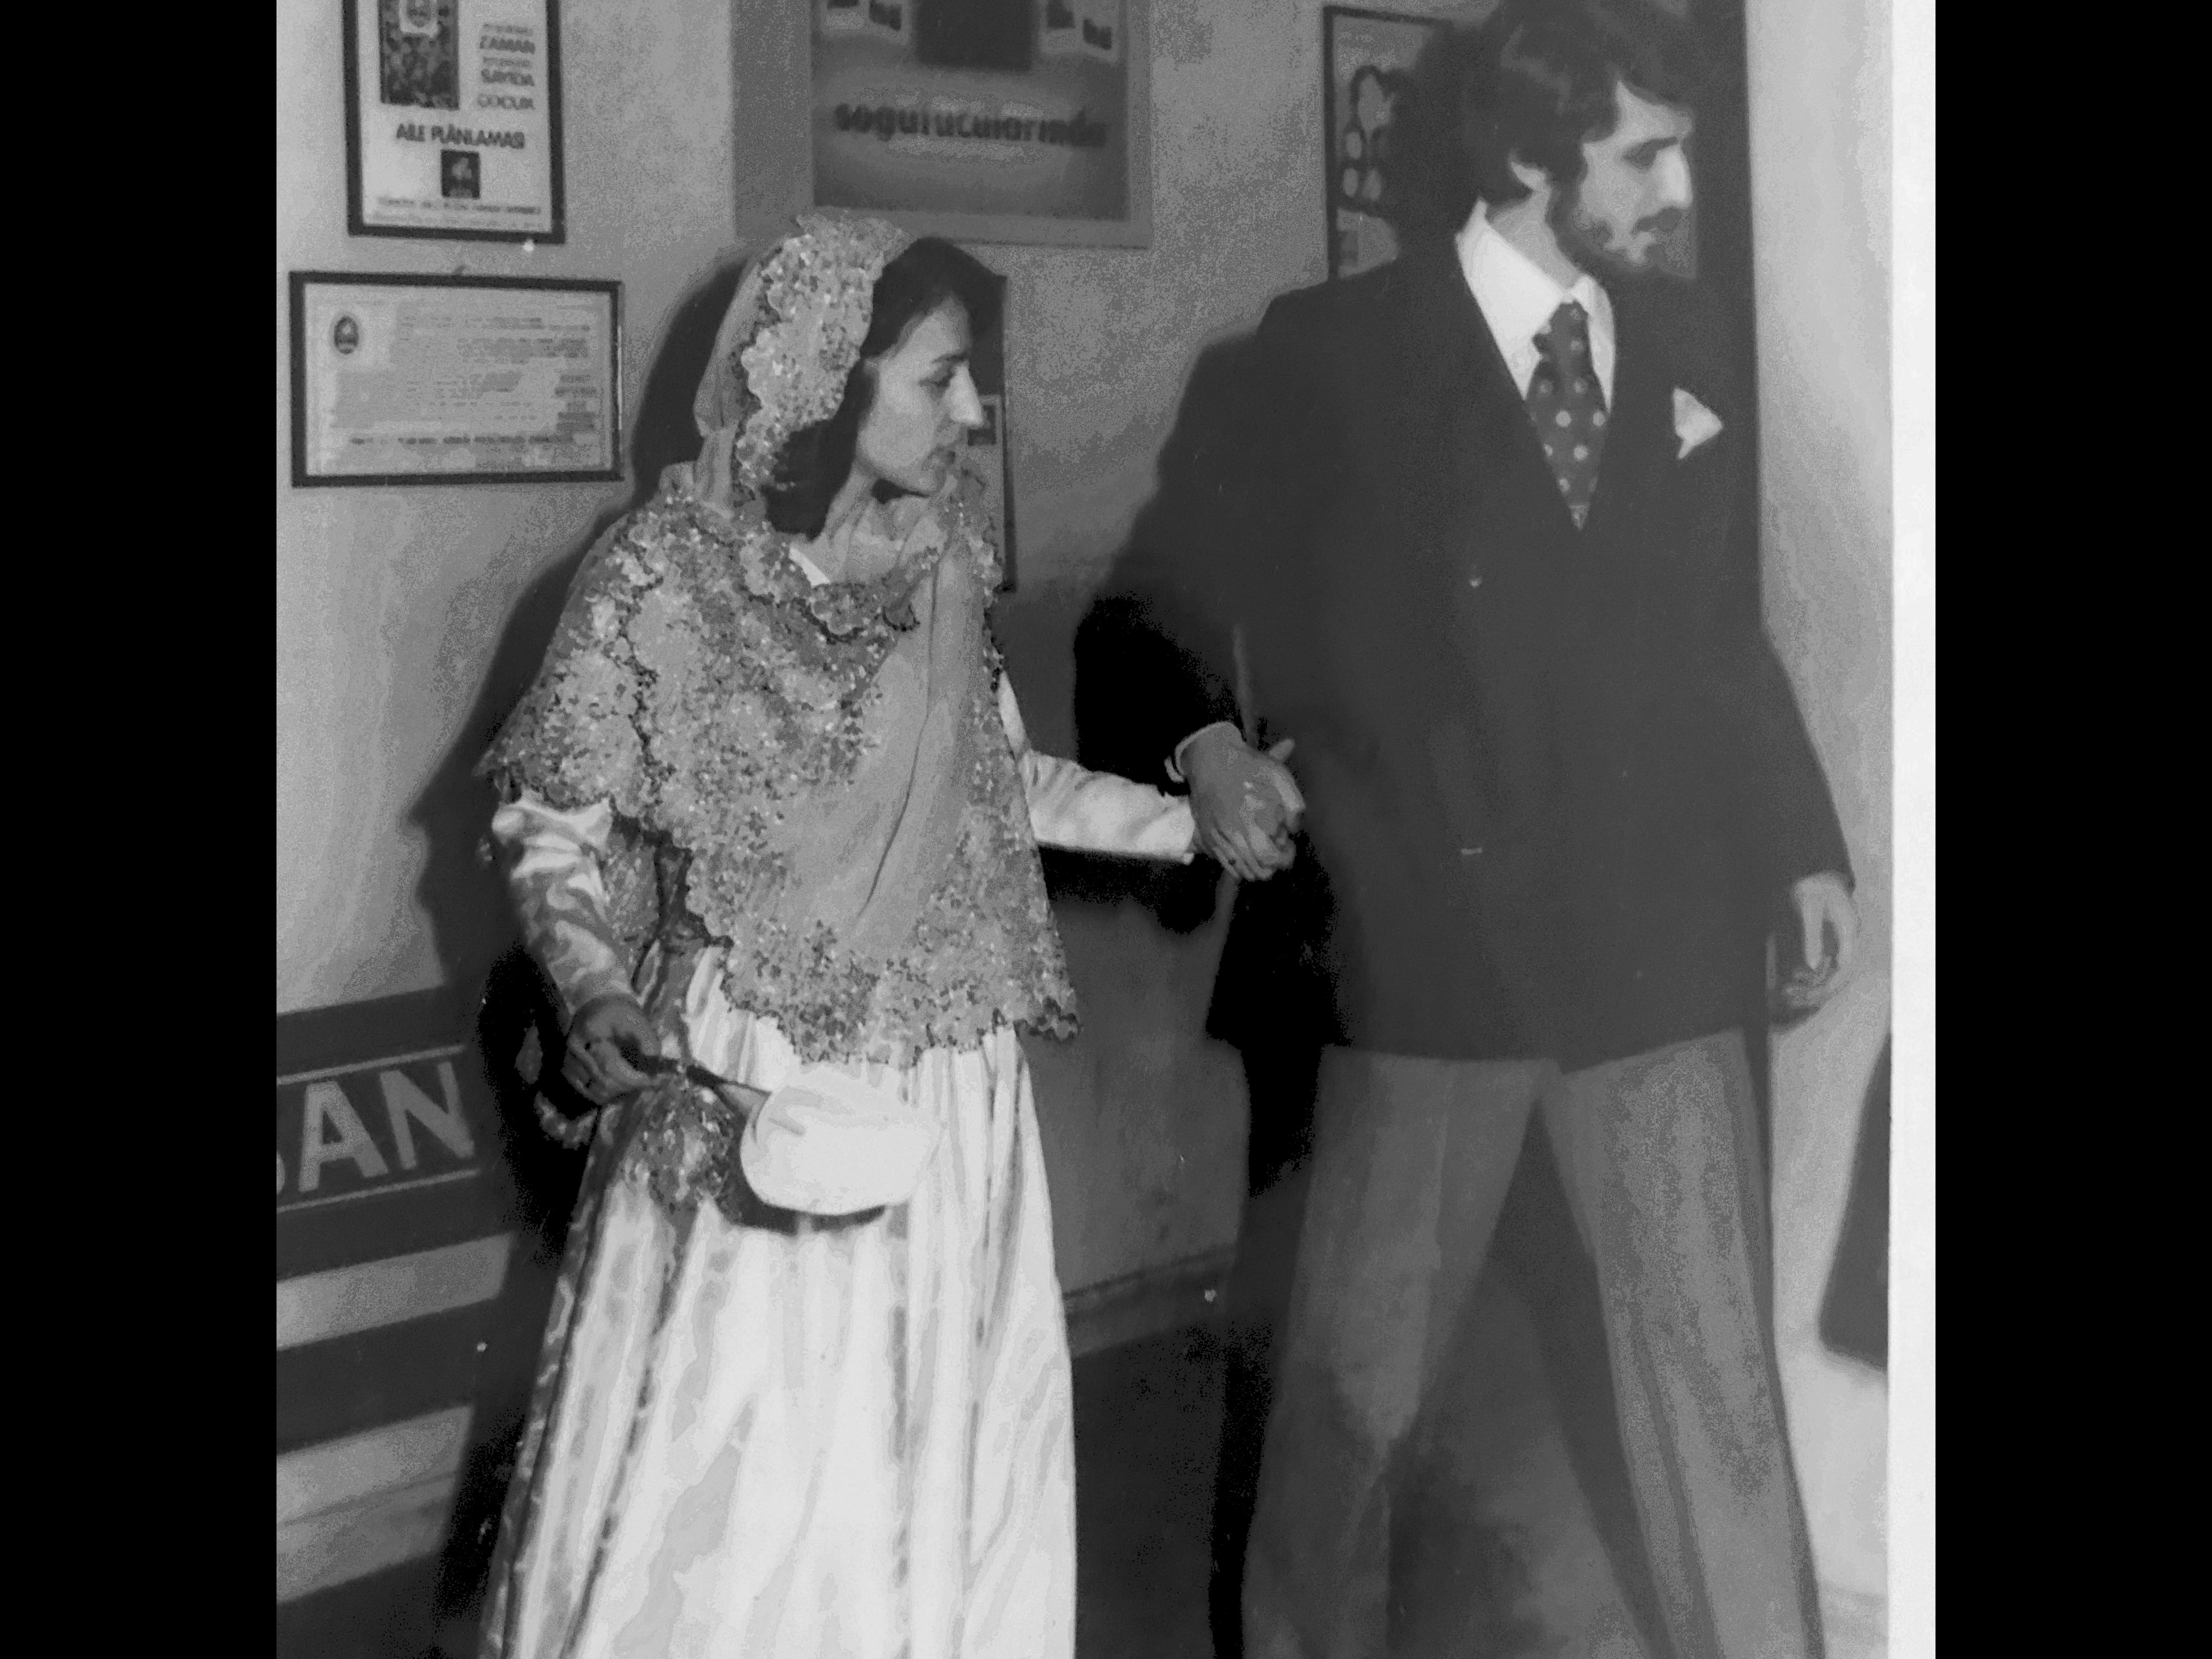
\includegraphics[width=0.3\linewidth]{1_G.jpg}
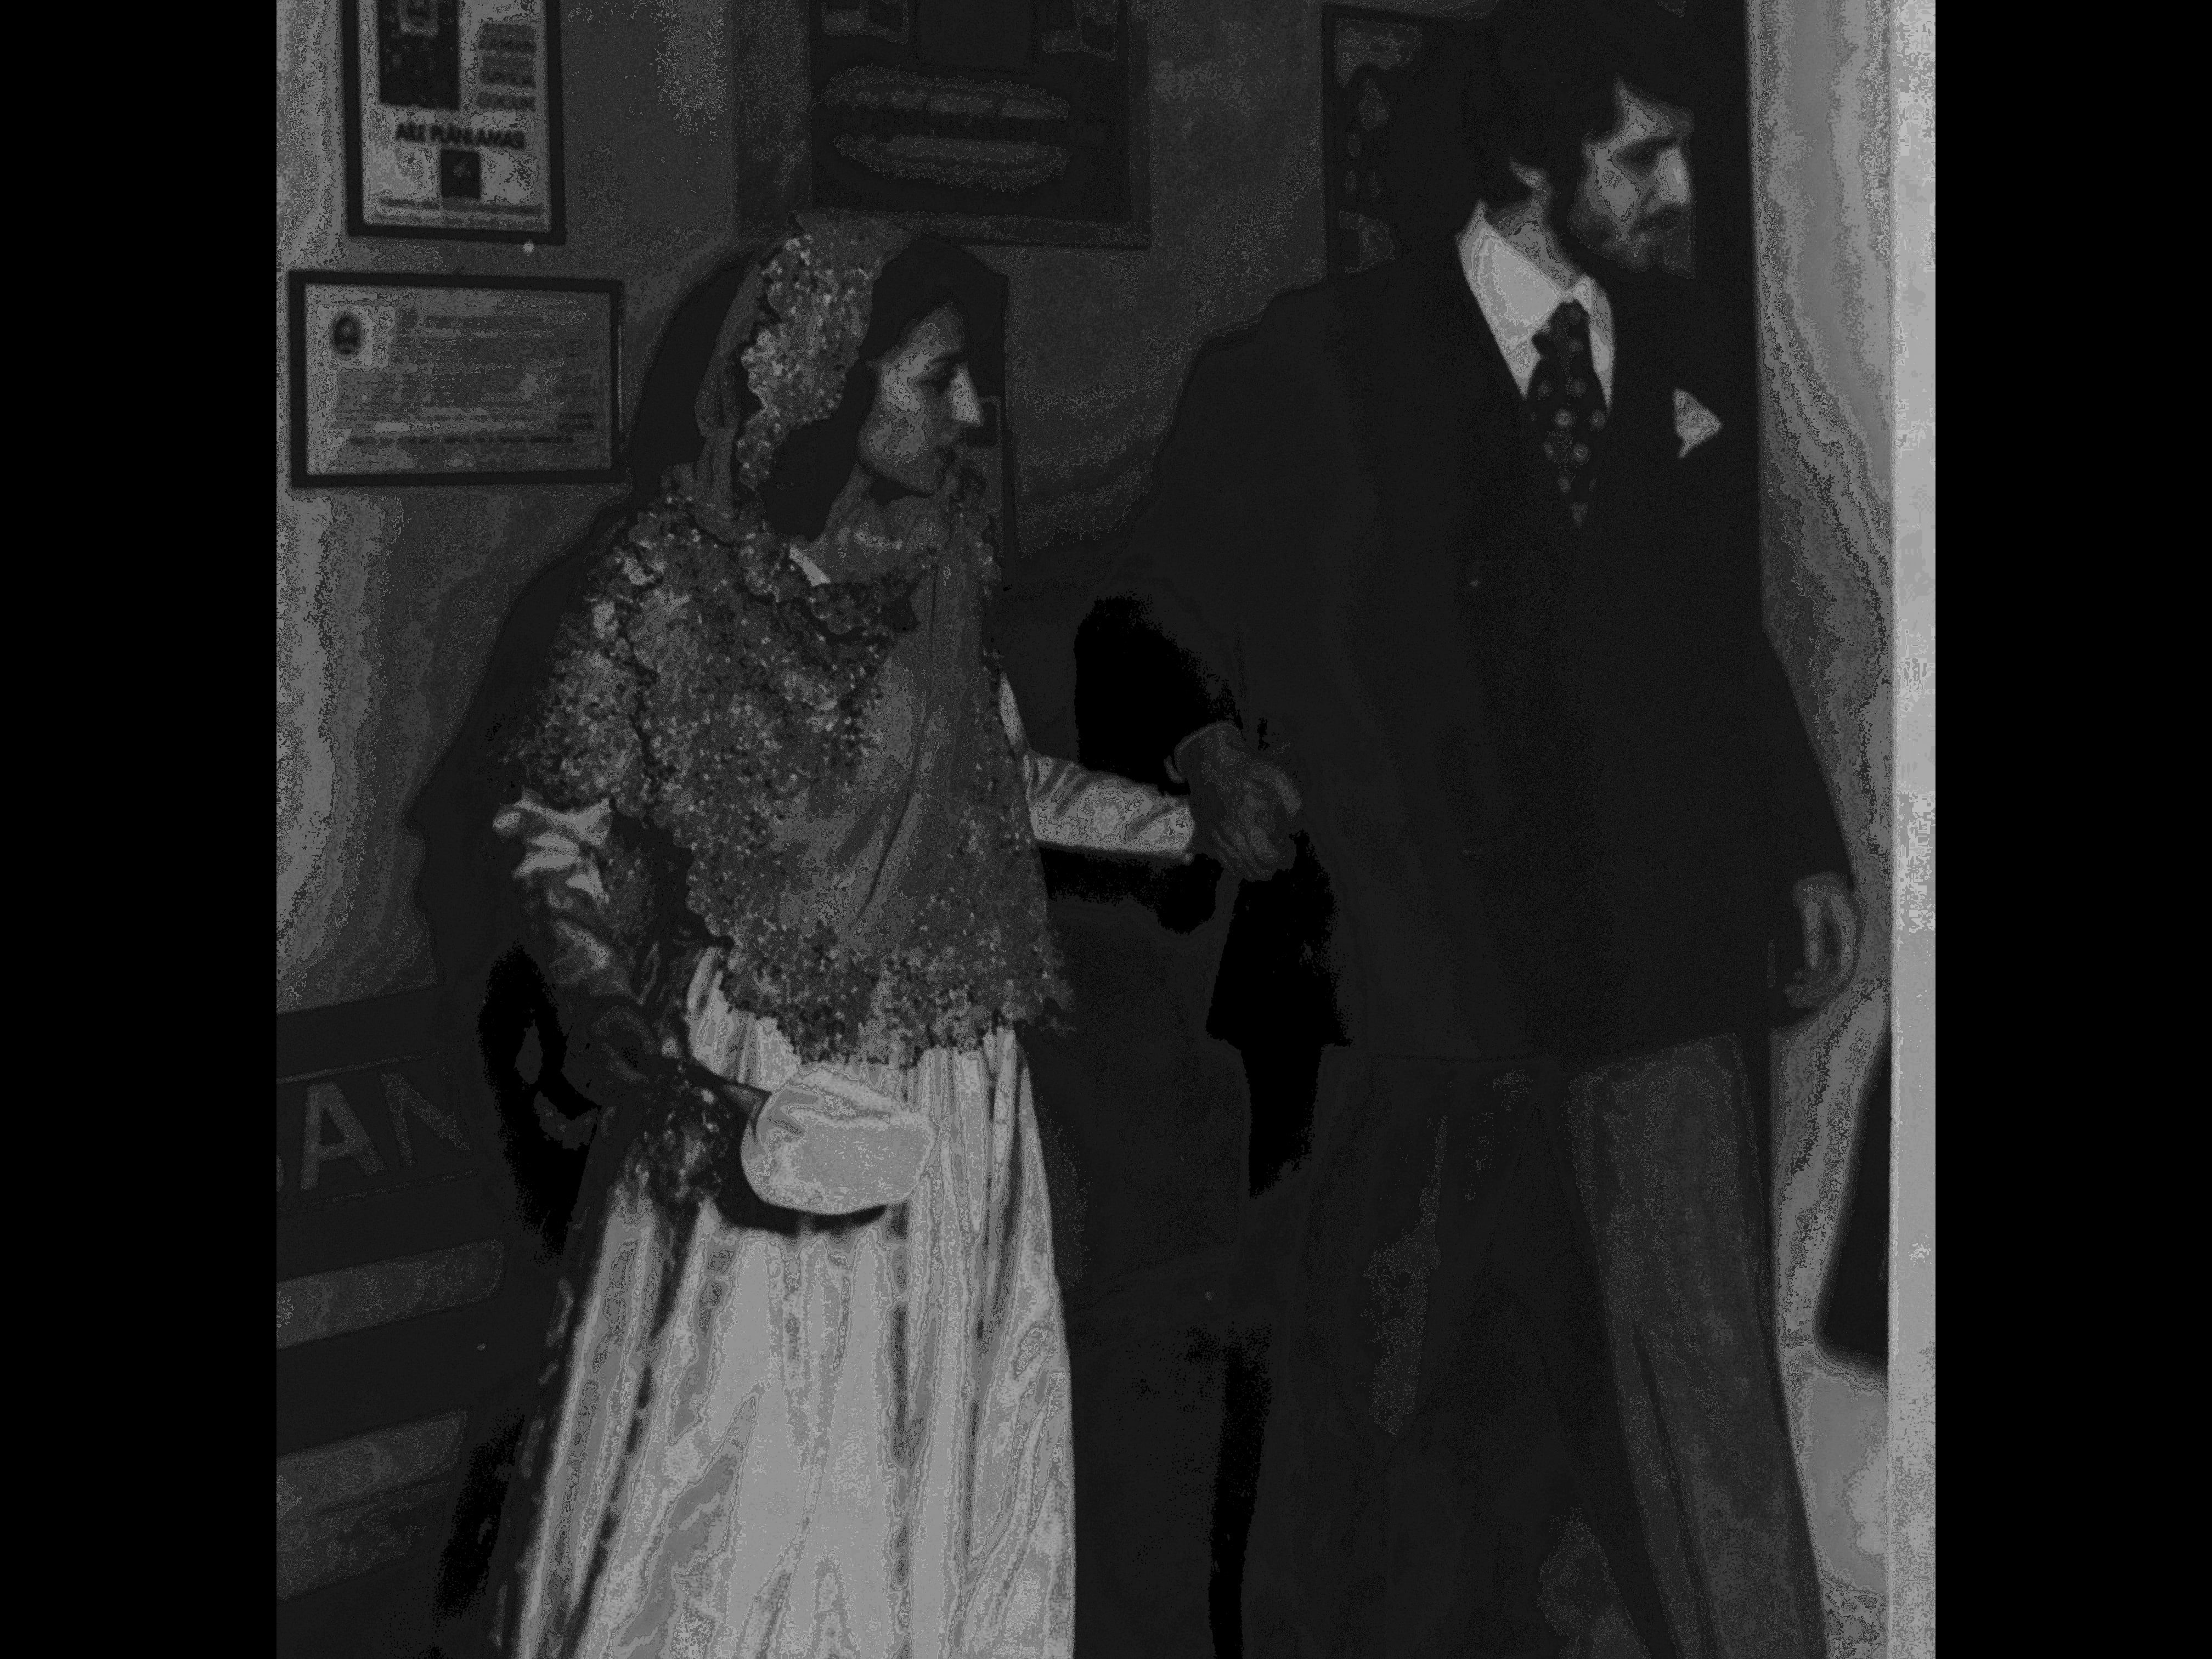
\includegraphics[width=0.3\linewidth]{1_B.jpg}
\newline
H, S, I channels as the result of pseudo-coloring for image 1: \\
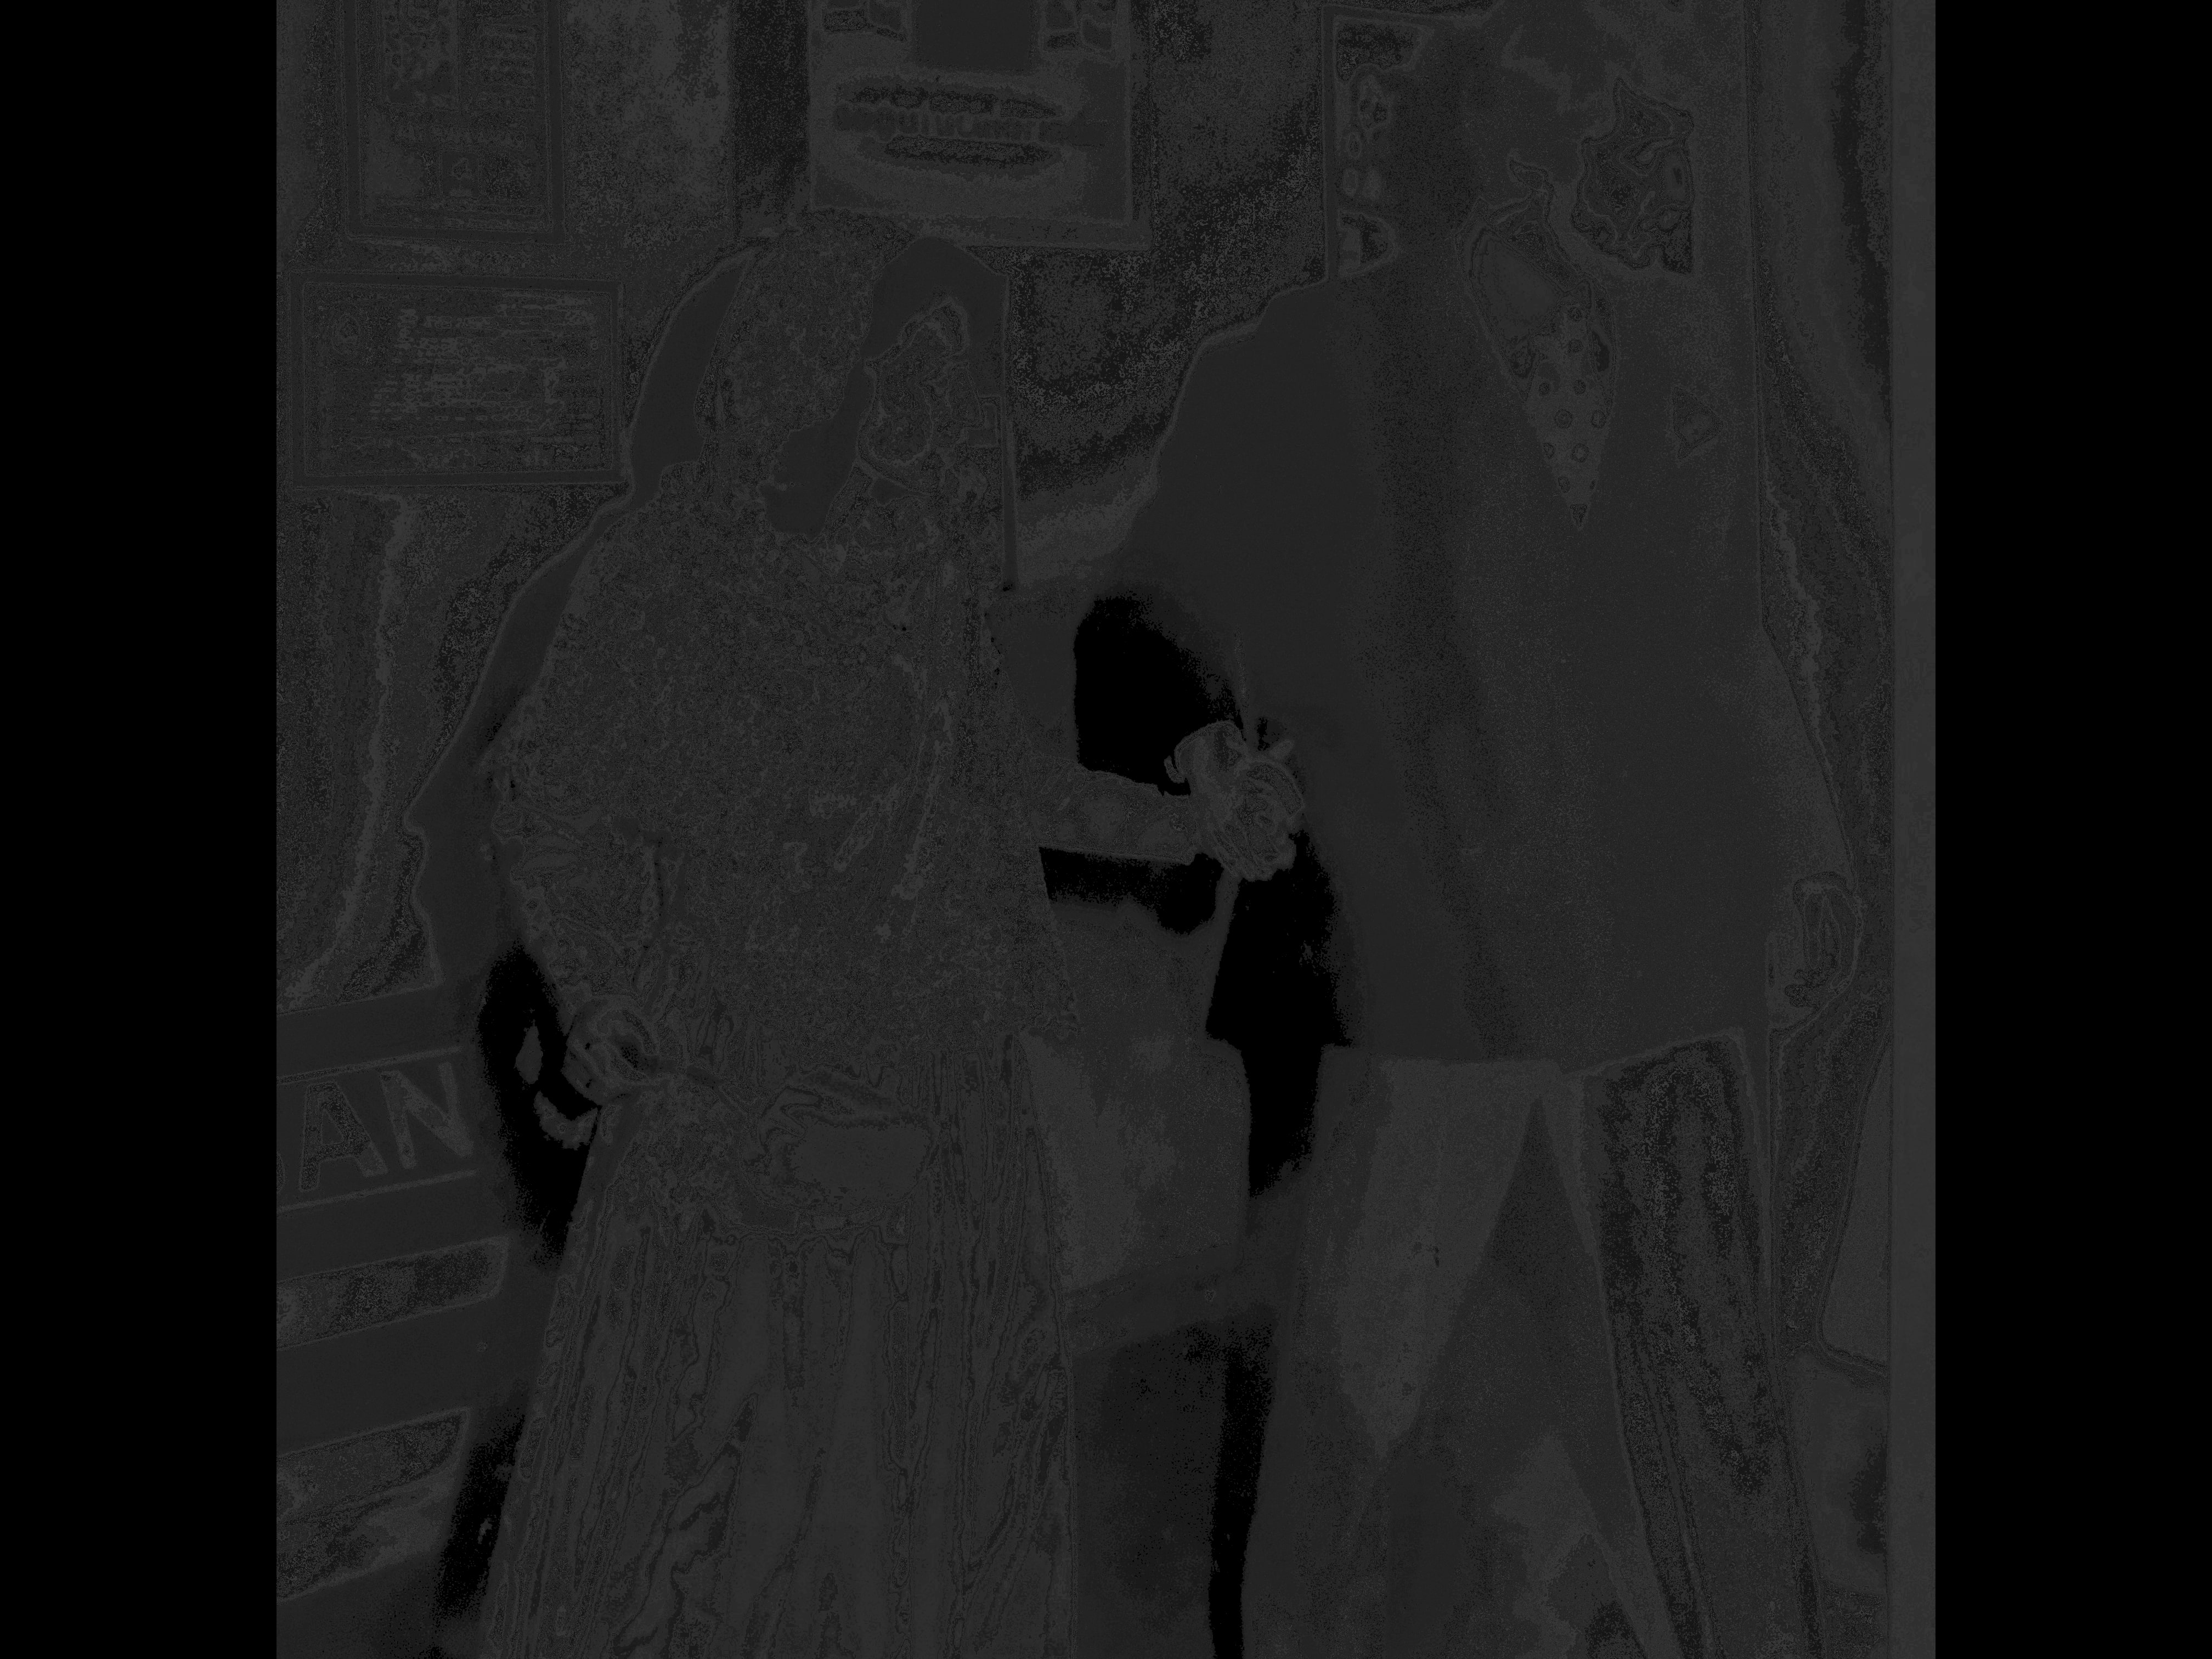
\includegraphics[width=0.3\linewidth]{1_H.jpg}
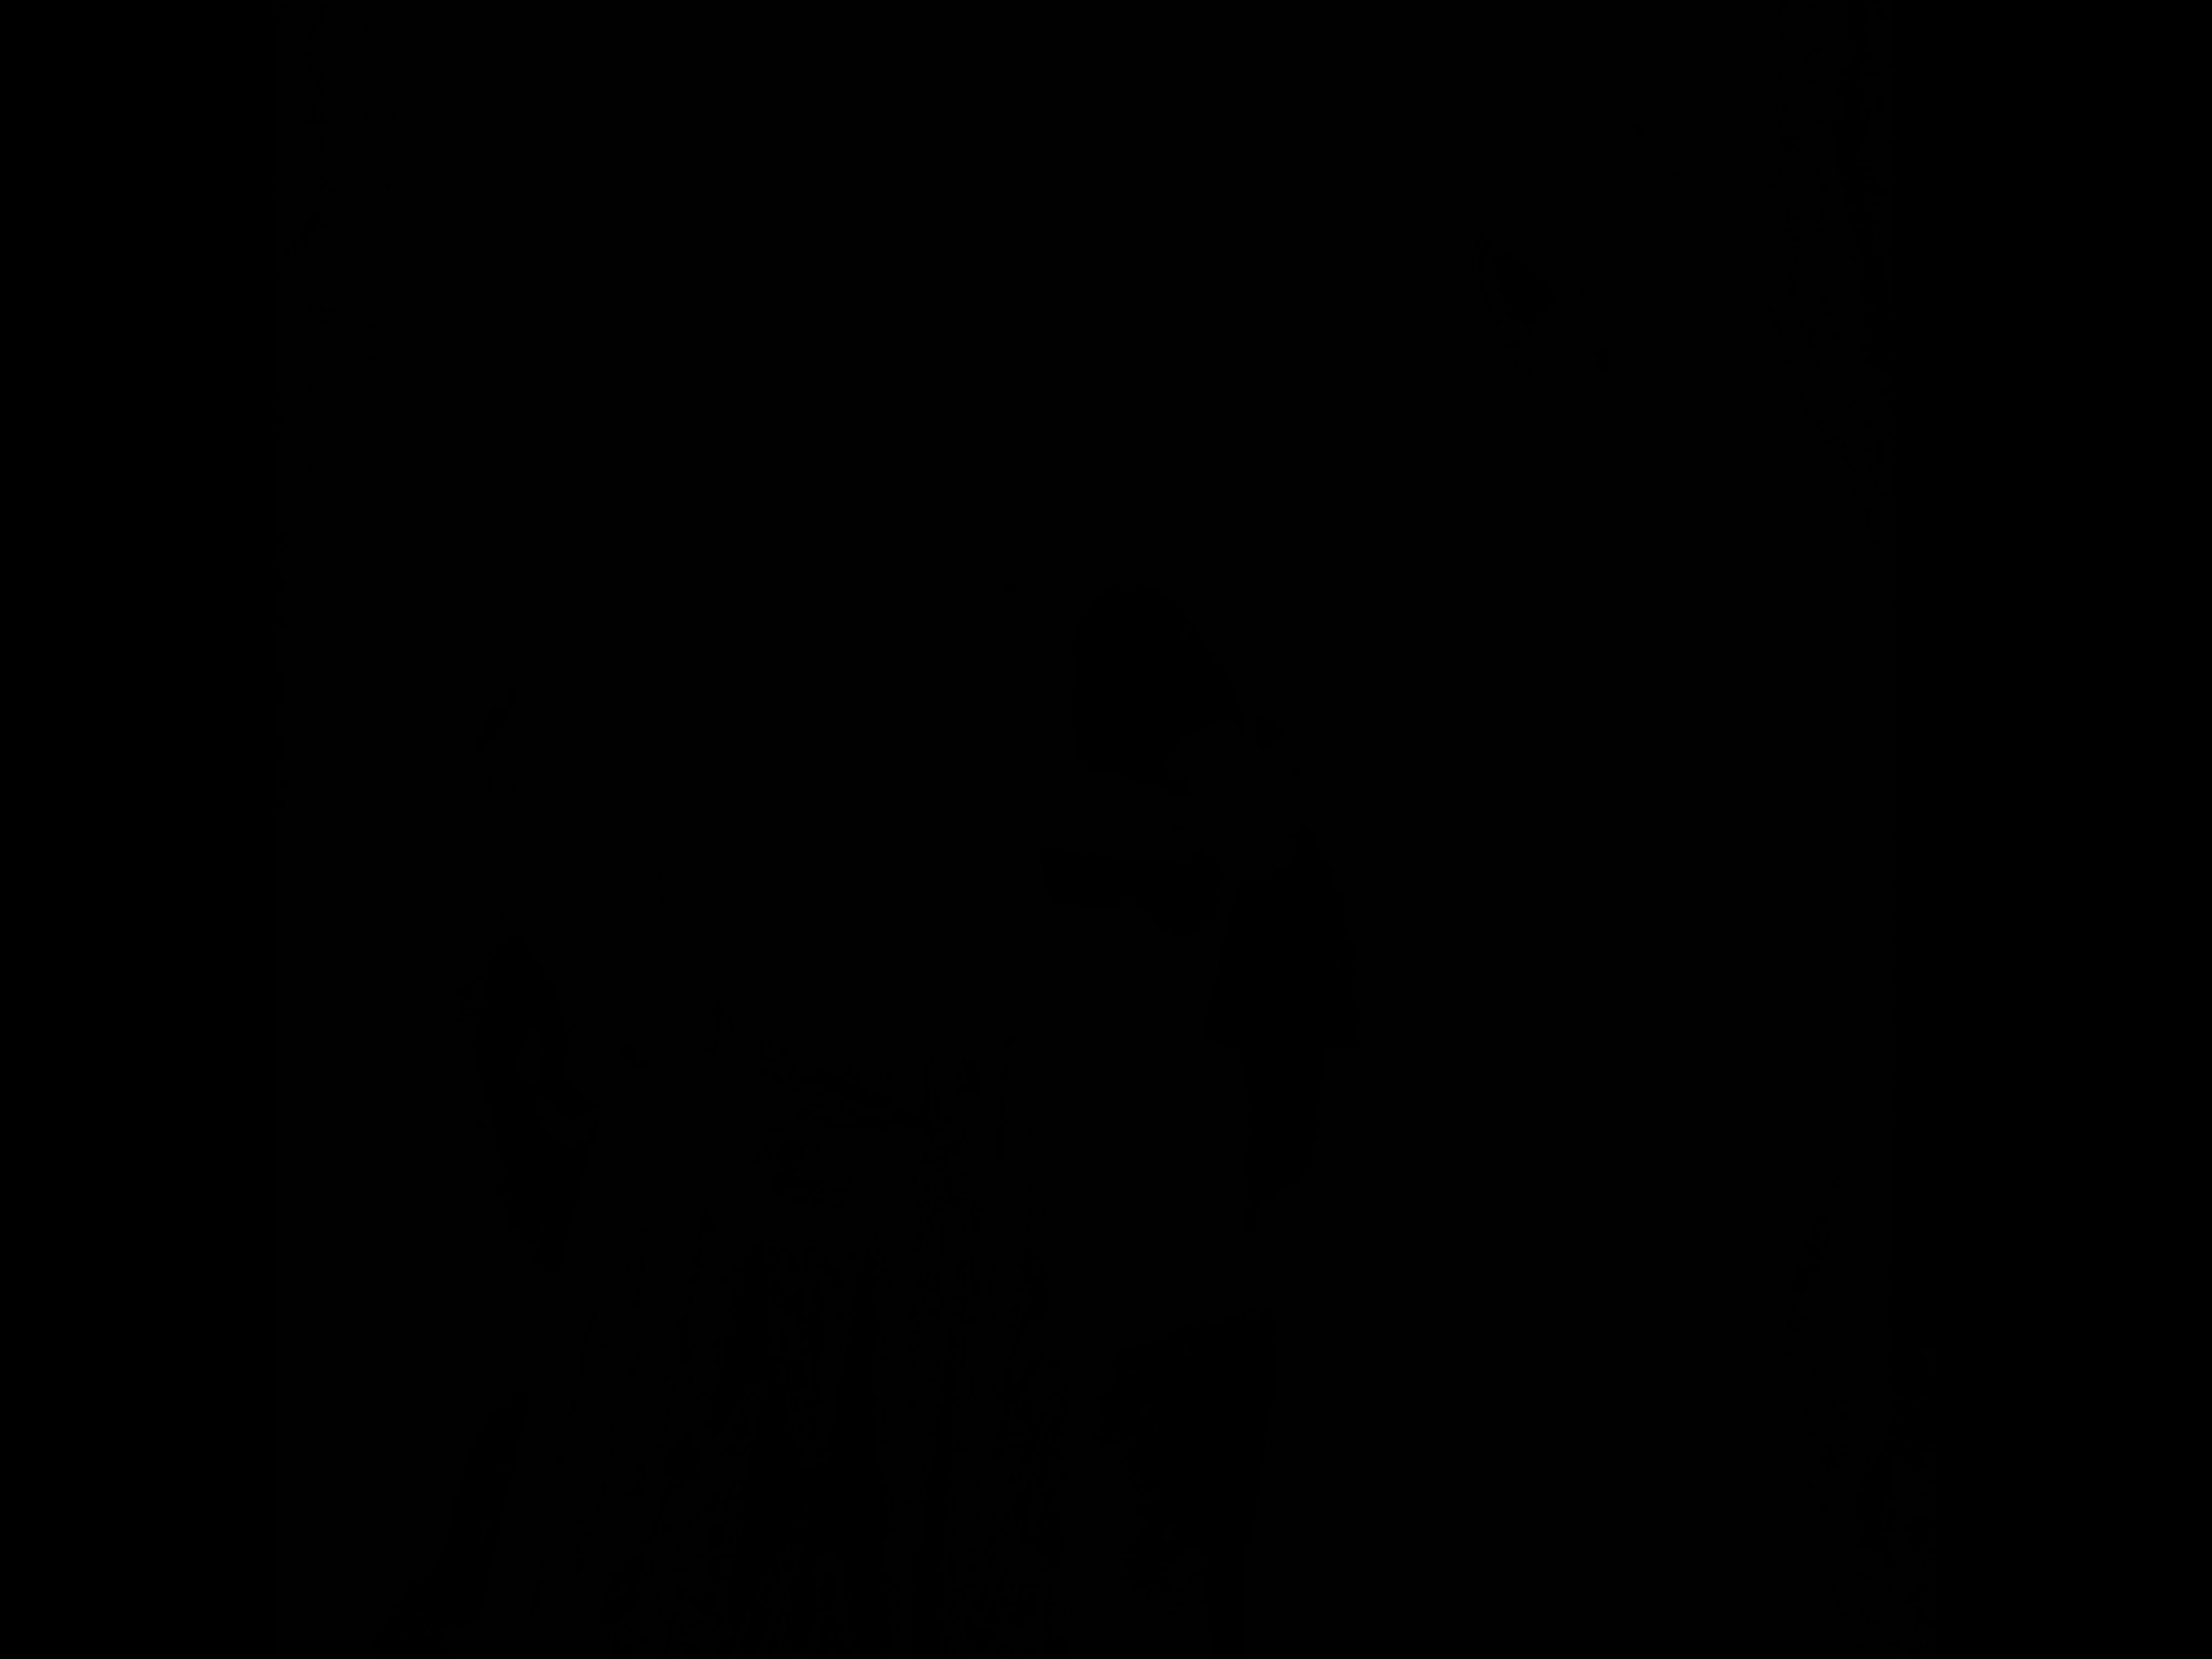
\includegraphics[width=0.3\linewidth]{1_S.jpg}
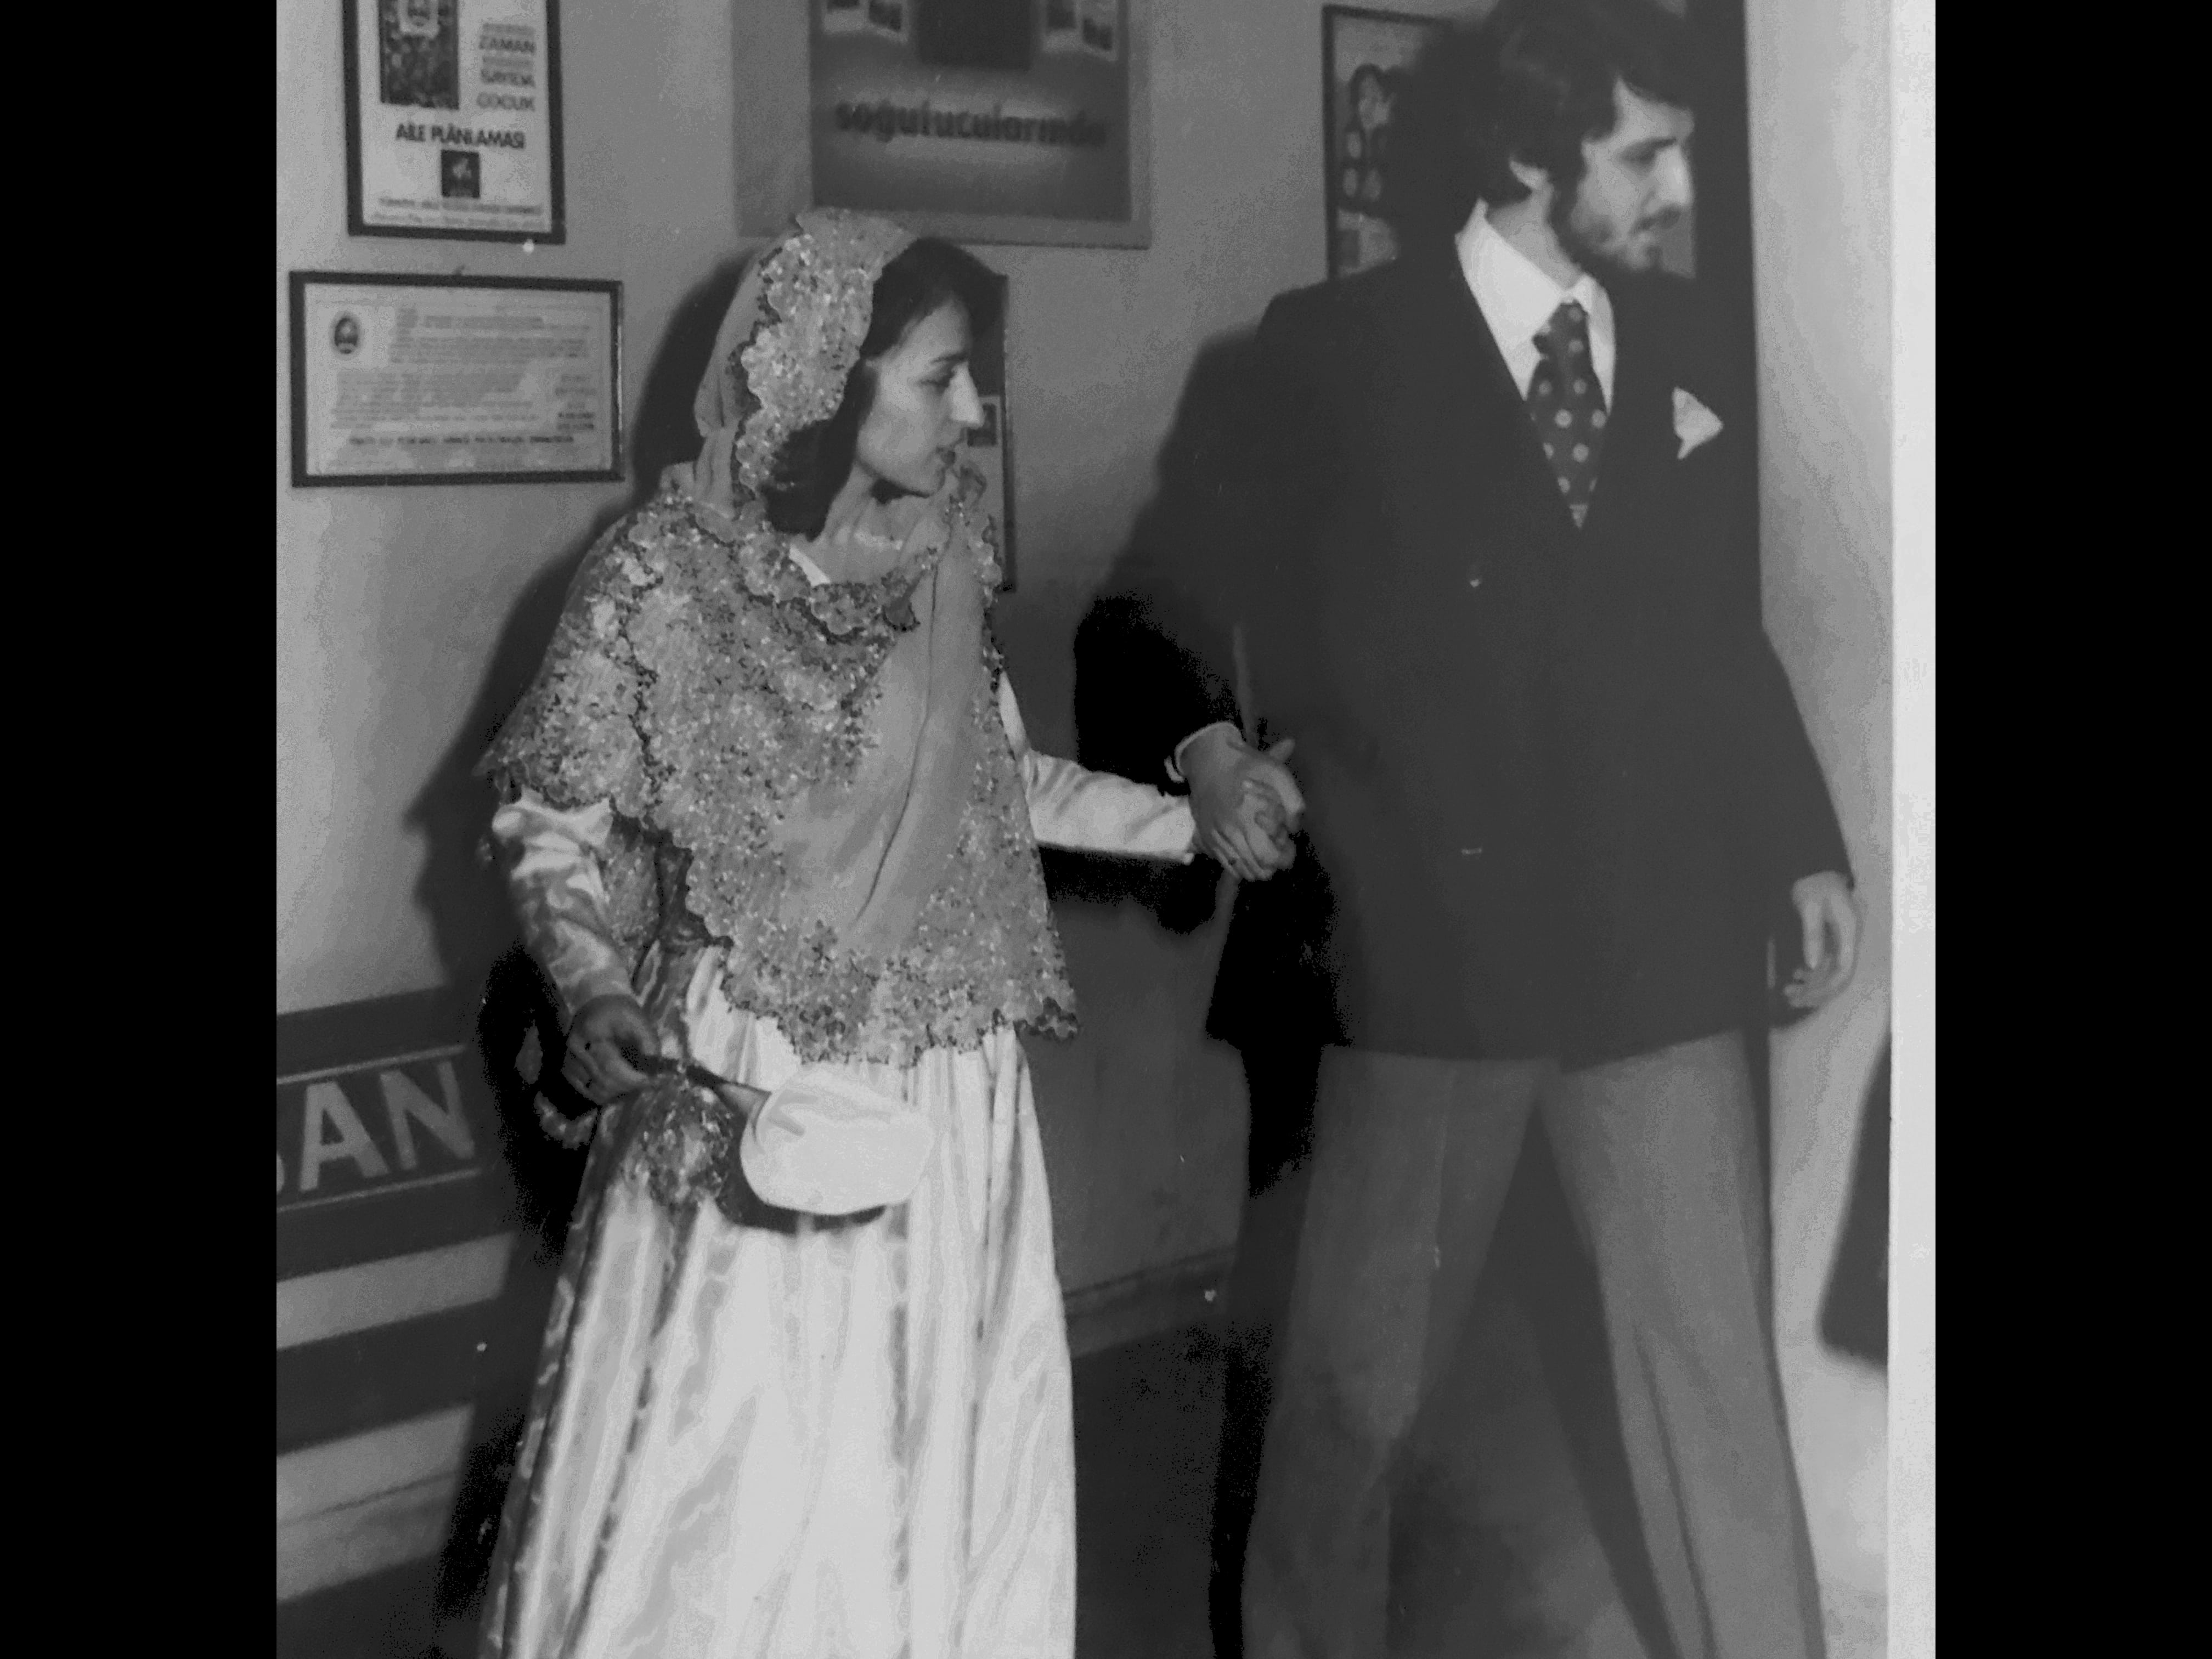
\includegraphics[width=0.3\linewidth]{1_I.jpg}
\newline
R, G, B channels as the result of pseudo-coloring for image 2: \\
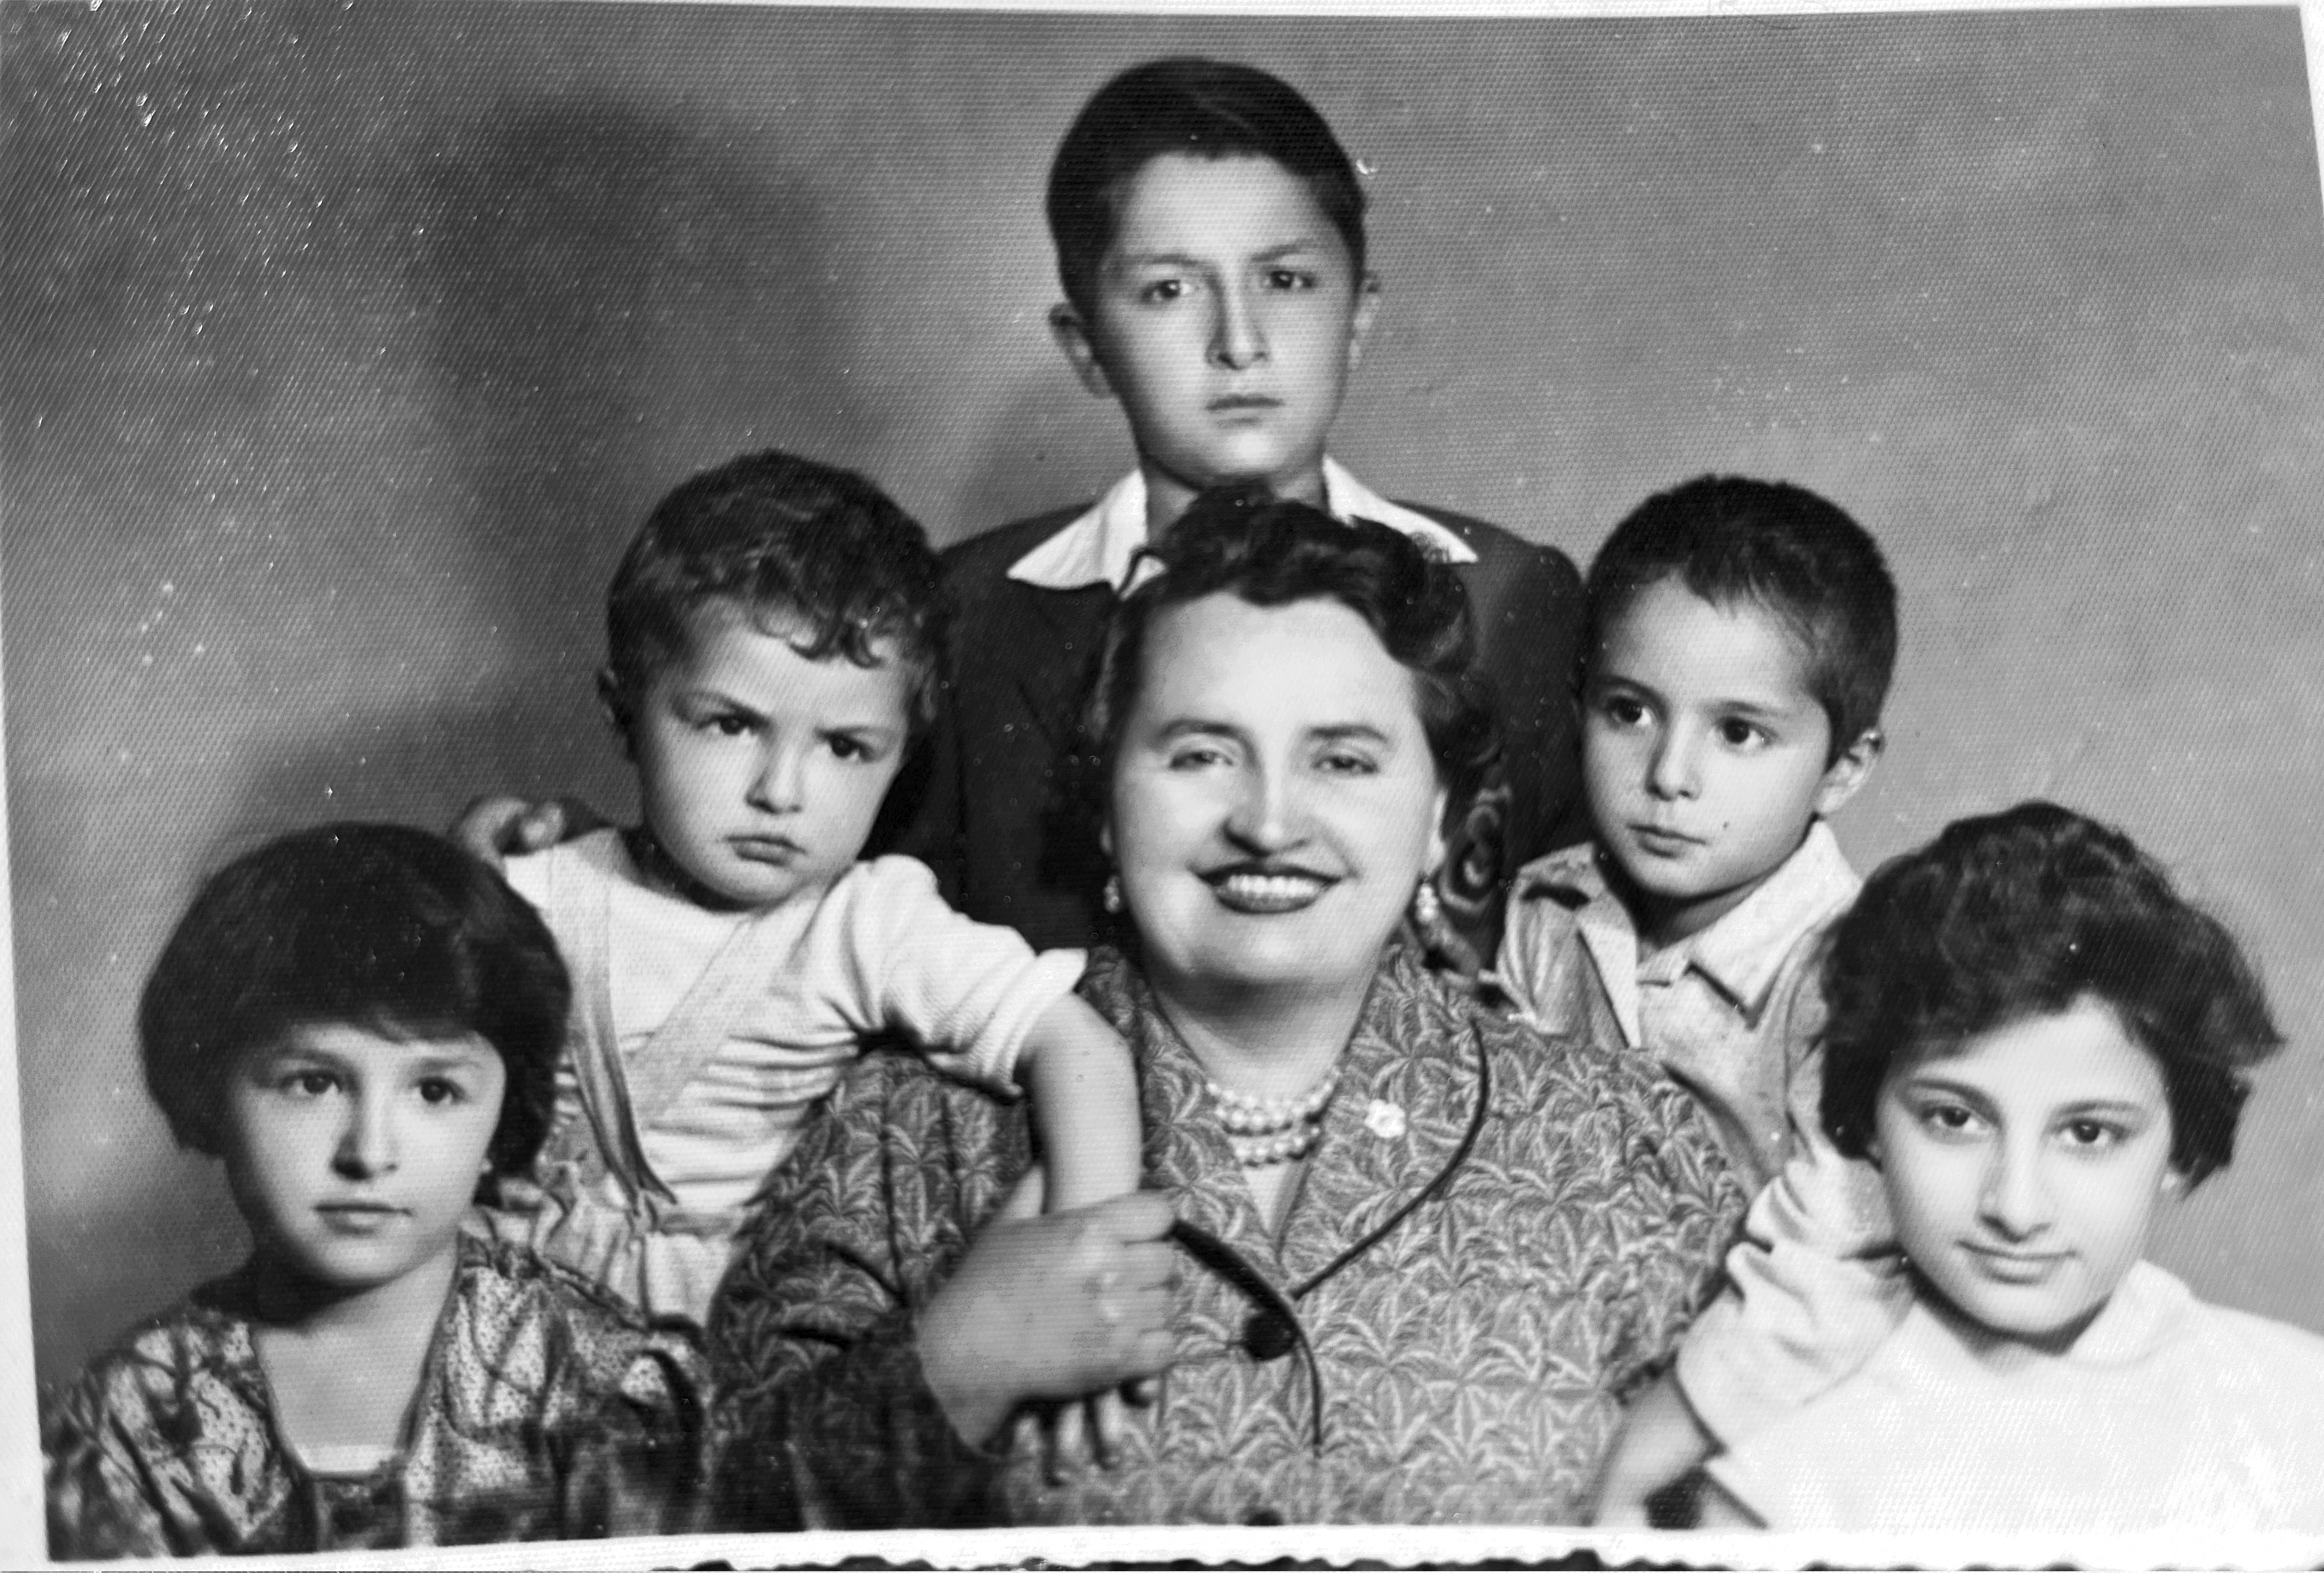
\includegraphics[width=0.3\linewidth]{2_R.jpg}
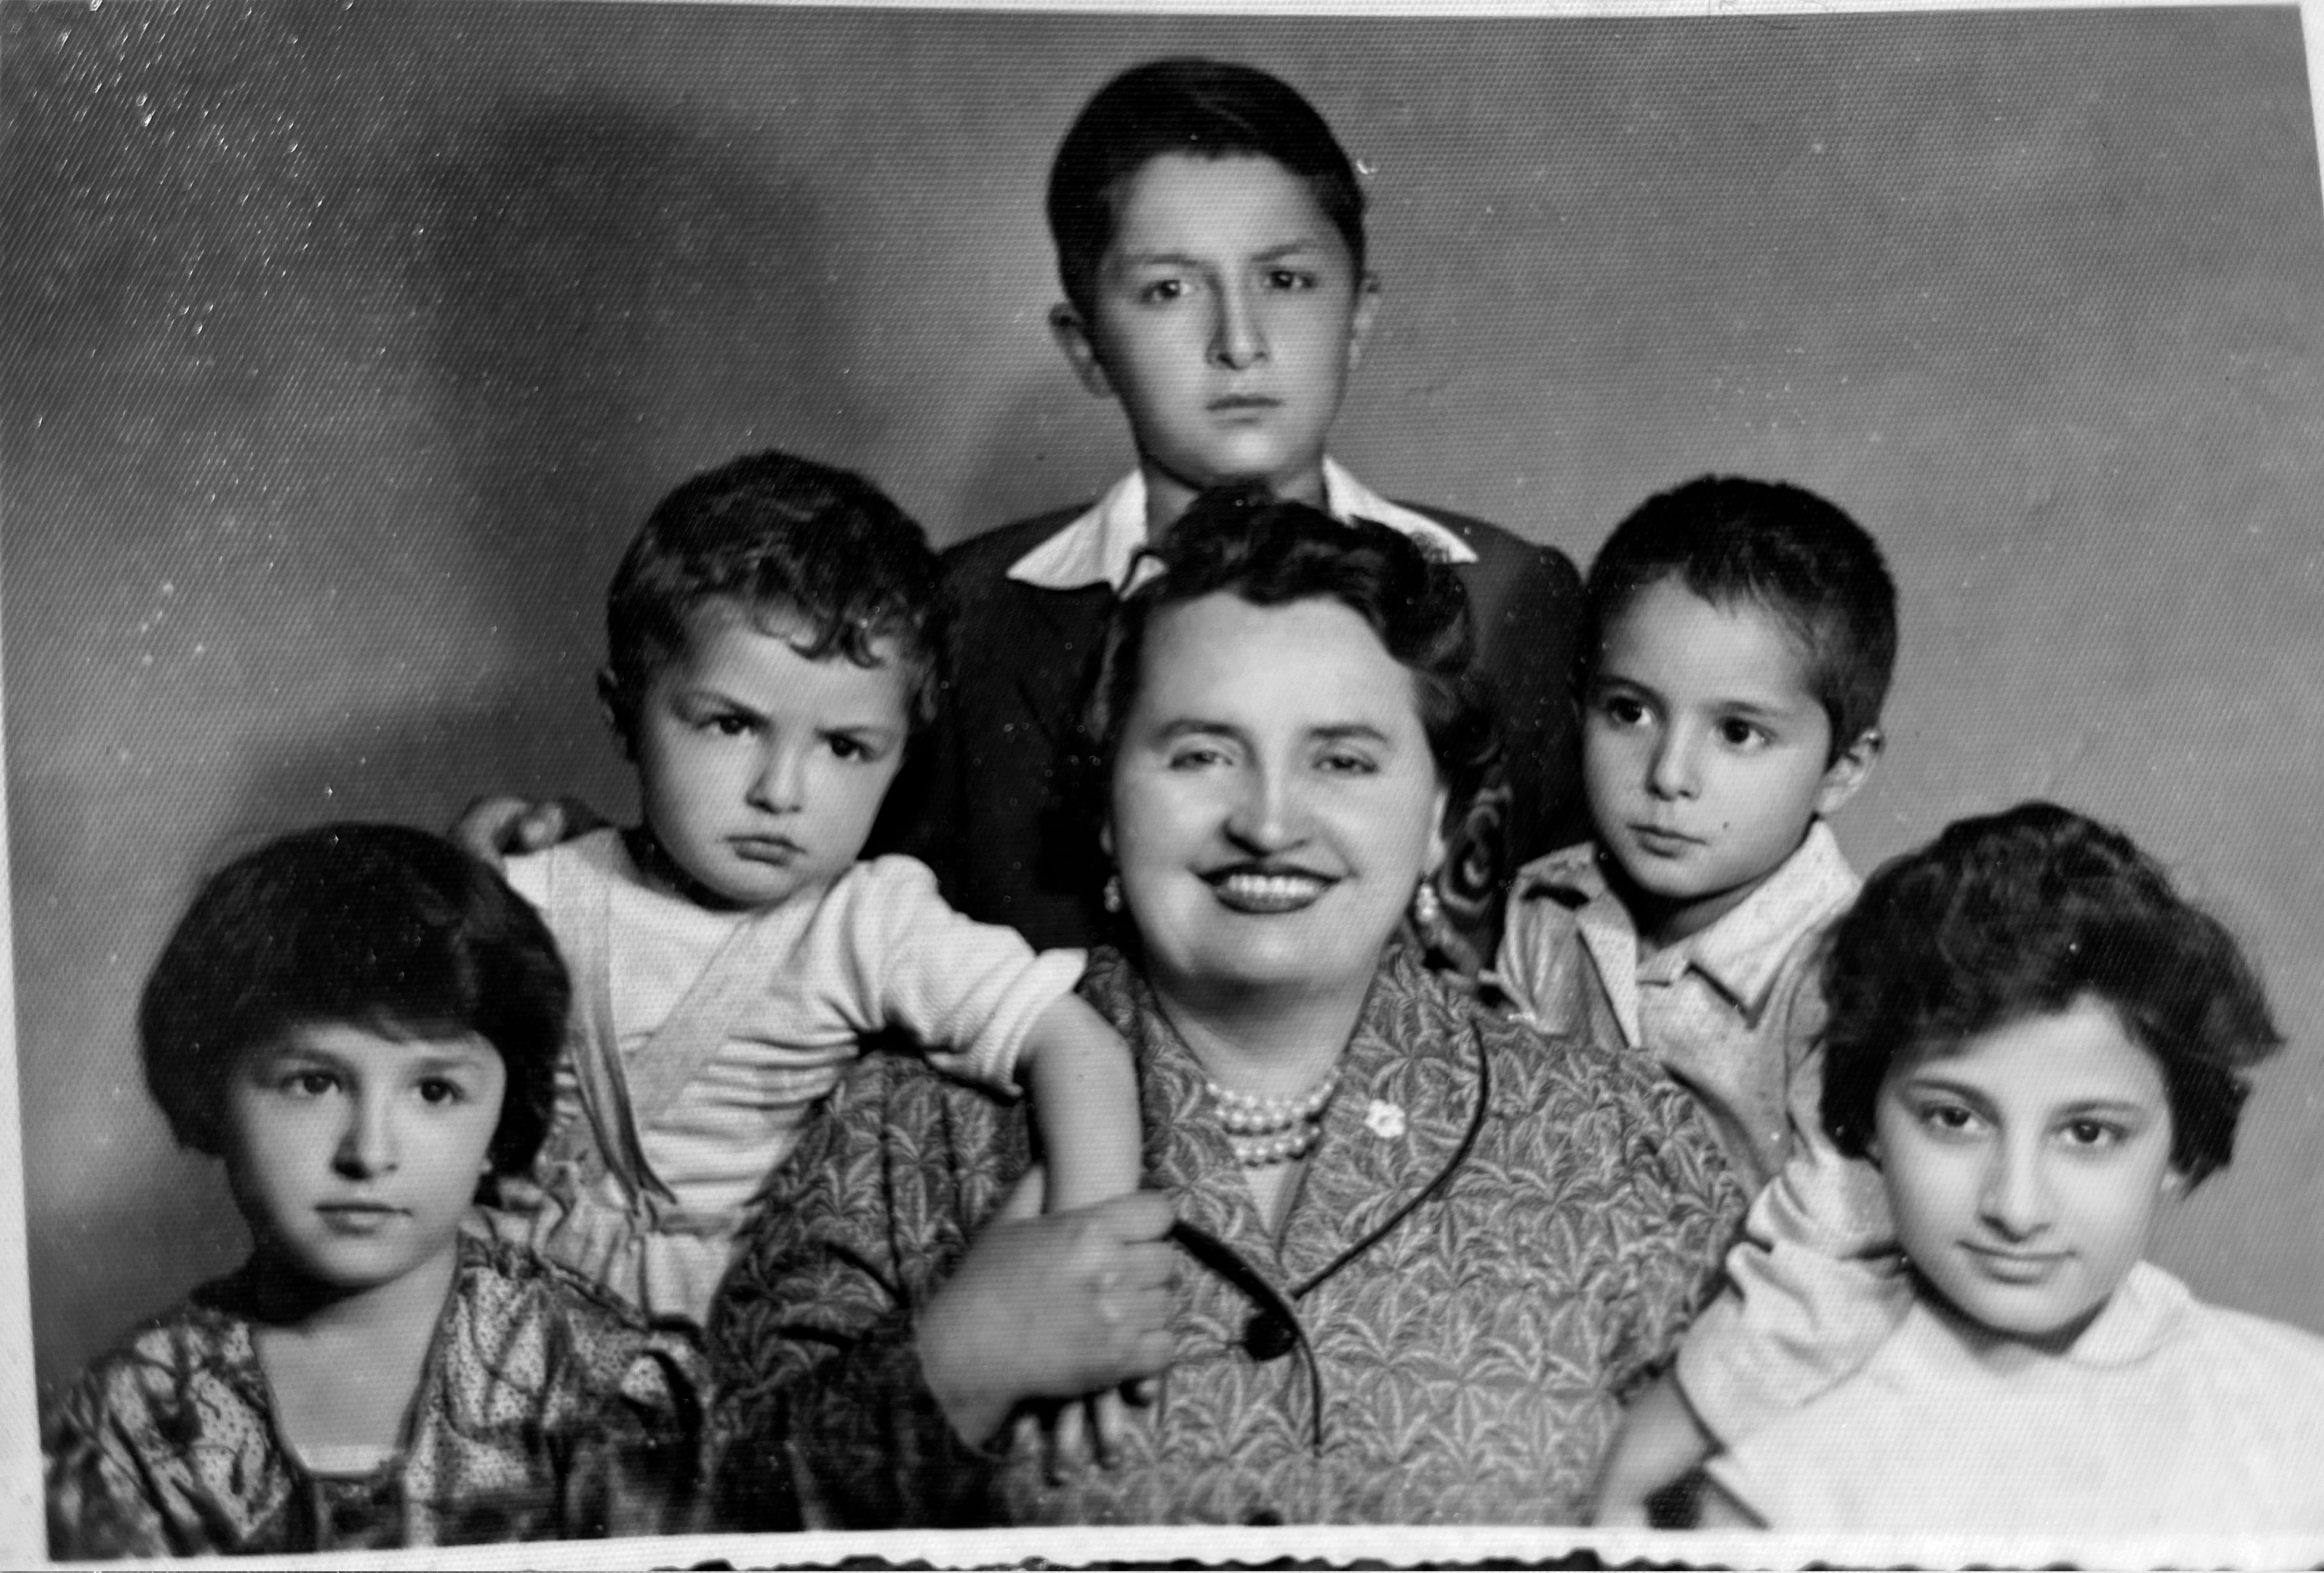
\includegraphics[width=0.3\linewidth]{2_G.jpg}
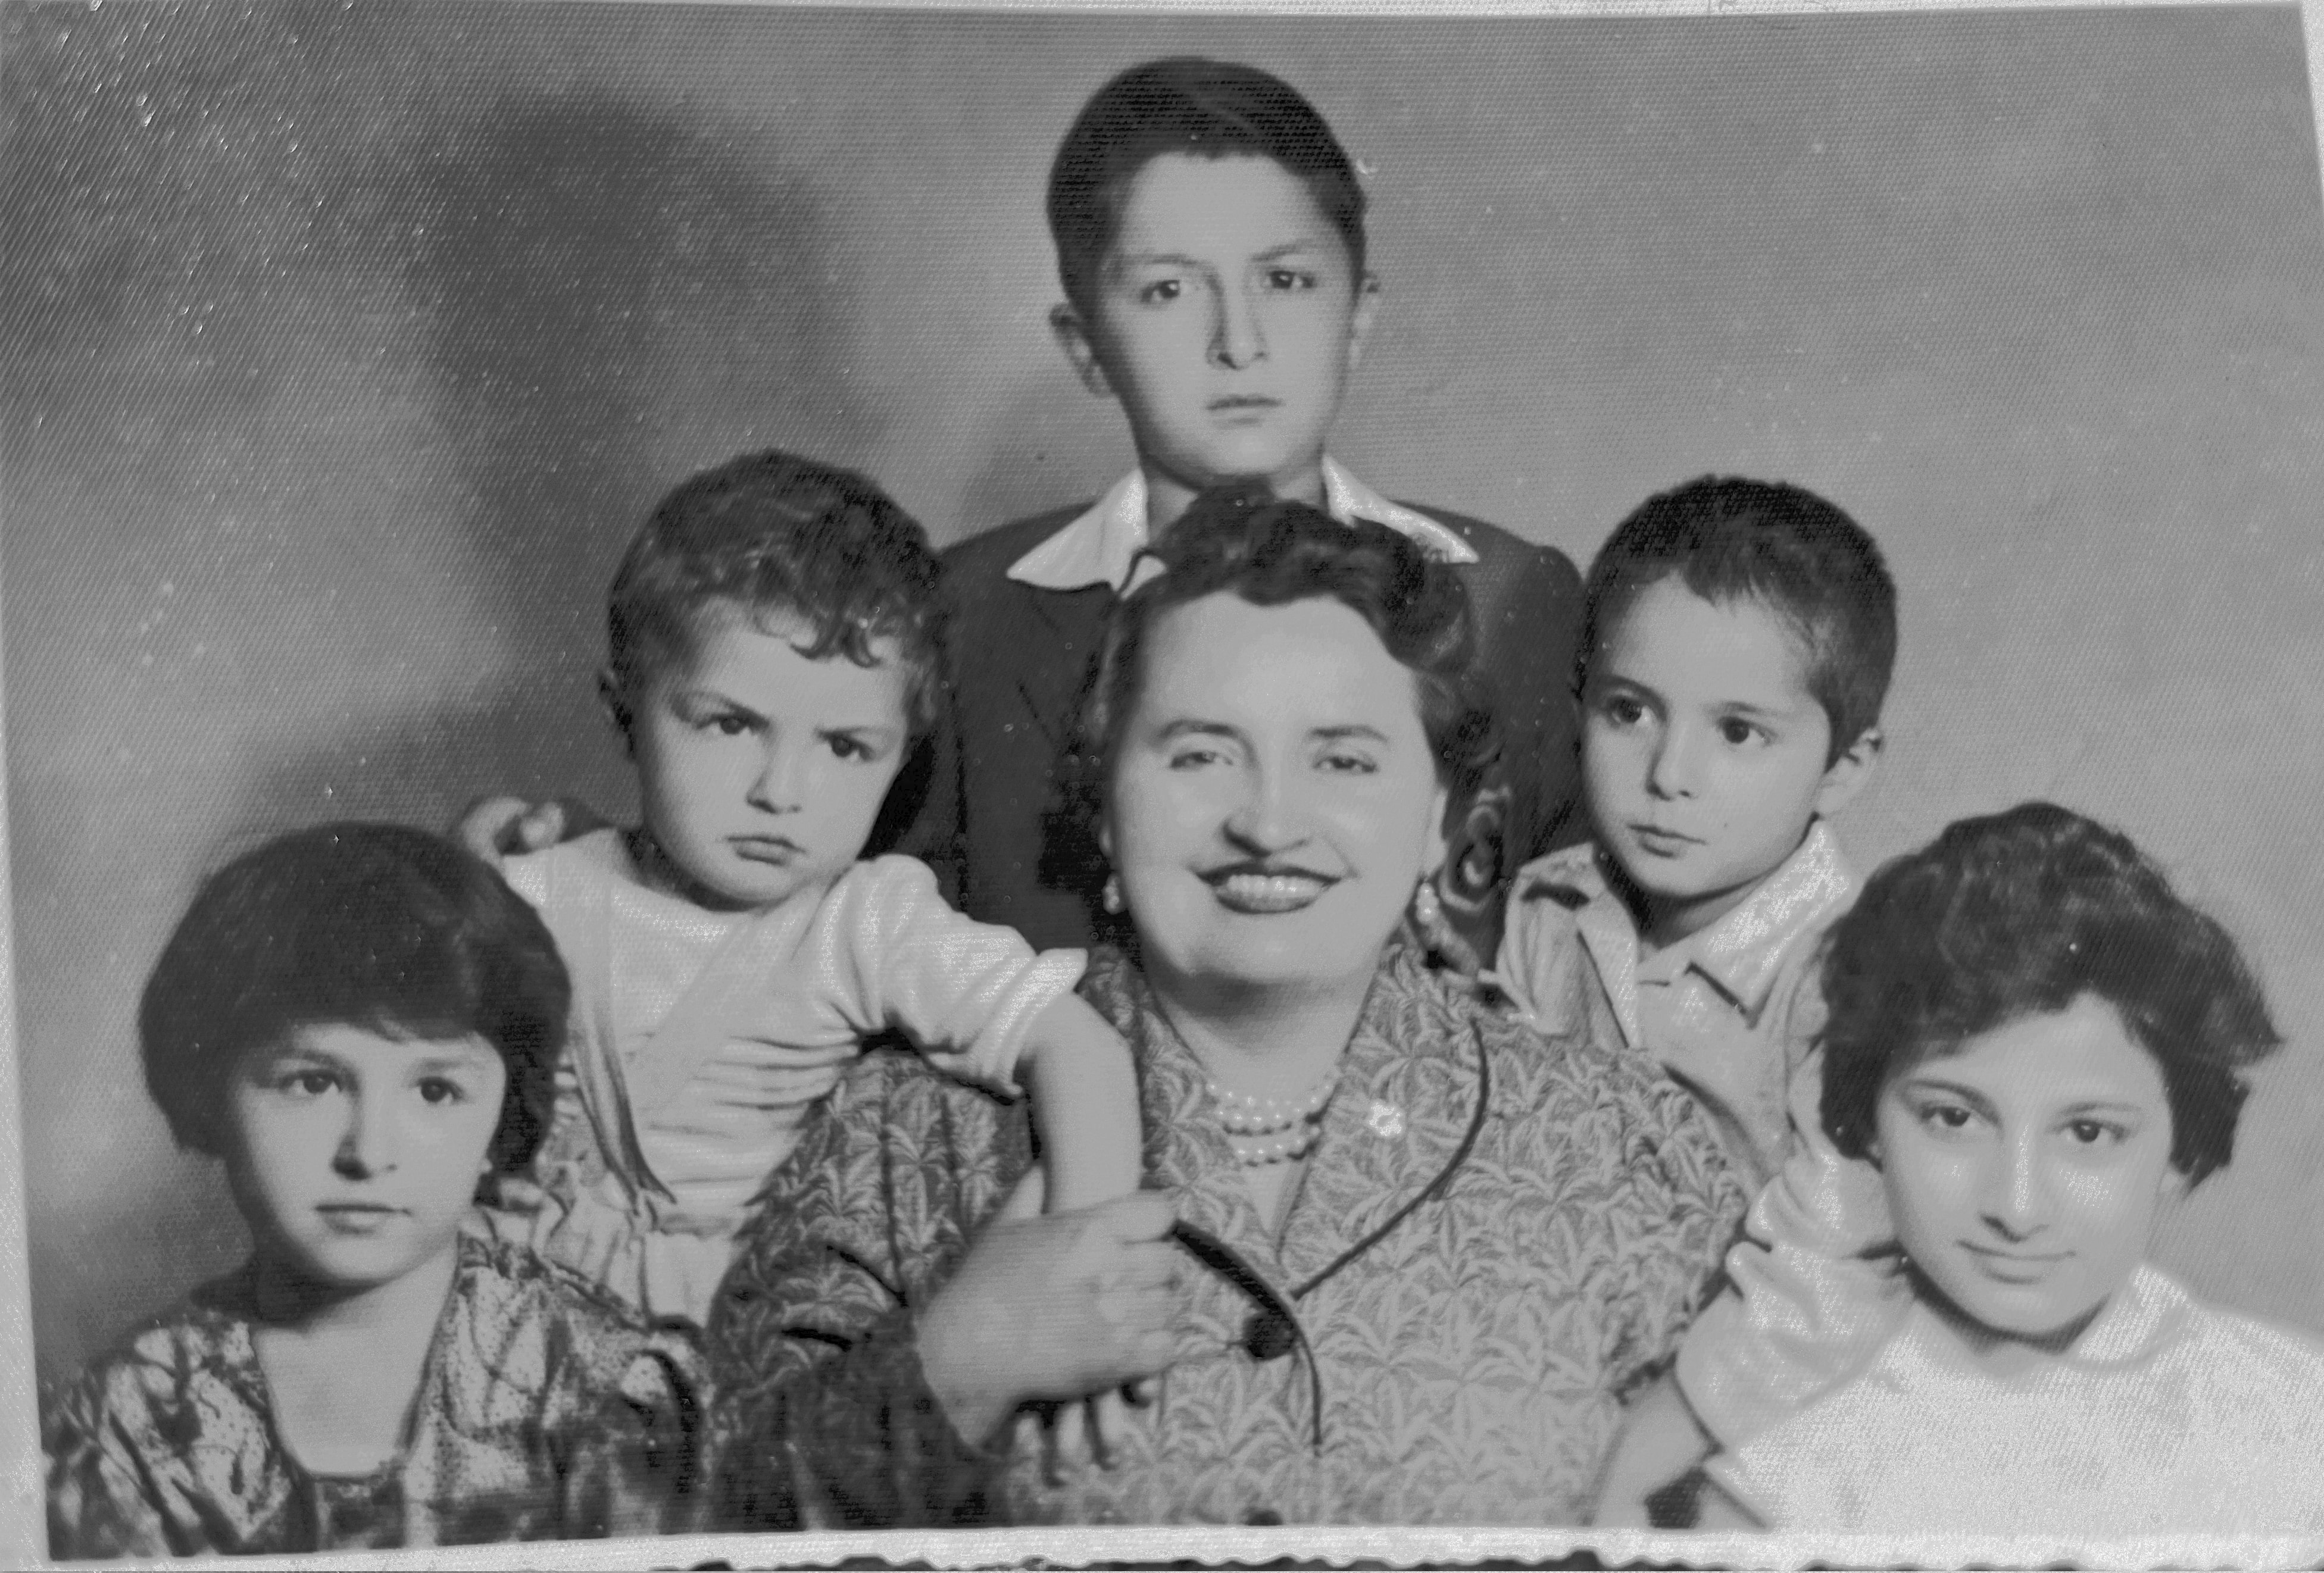
\includegraphics[width=0.3\linewidth]{2_B.jpg}
\newline
H, S, I channels as the result of pseudo-coloring for image 2: \\
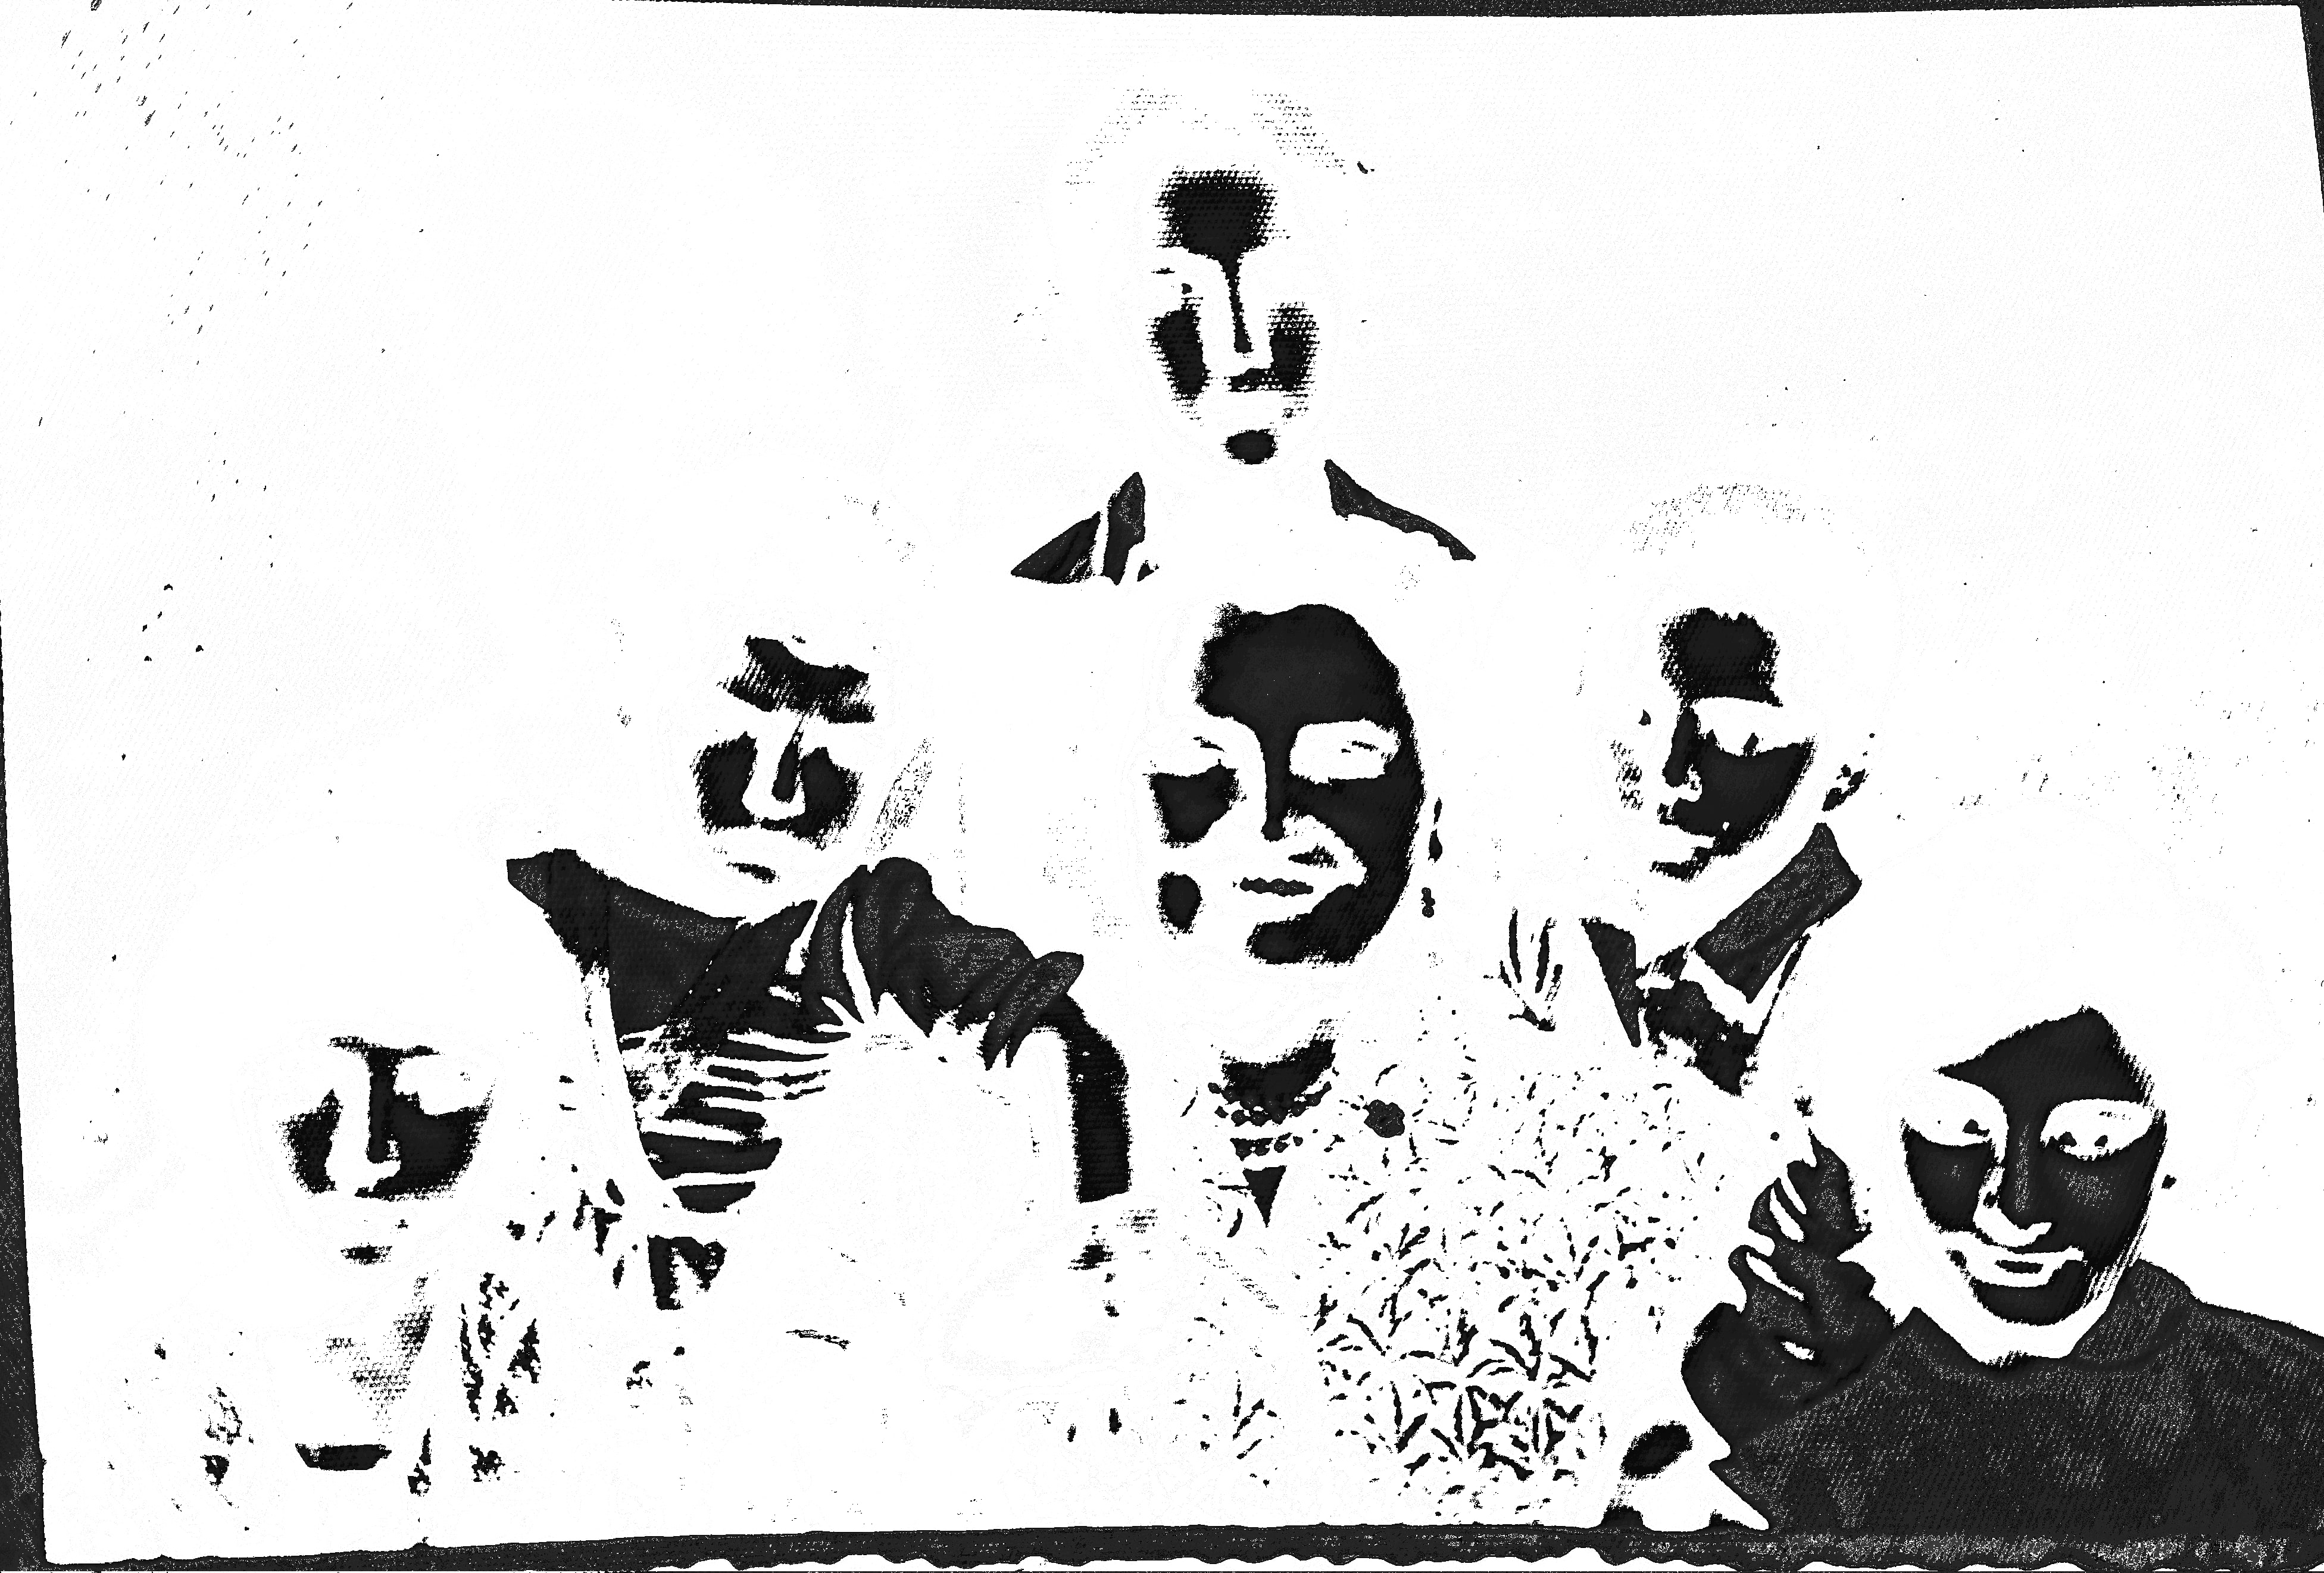
\includegraphics[width=0.3\linewidth]{2_H.jpg}
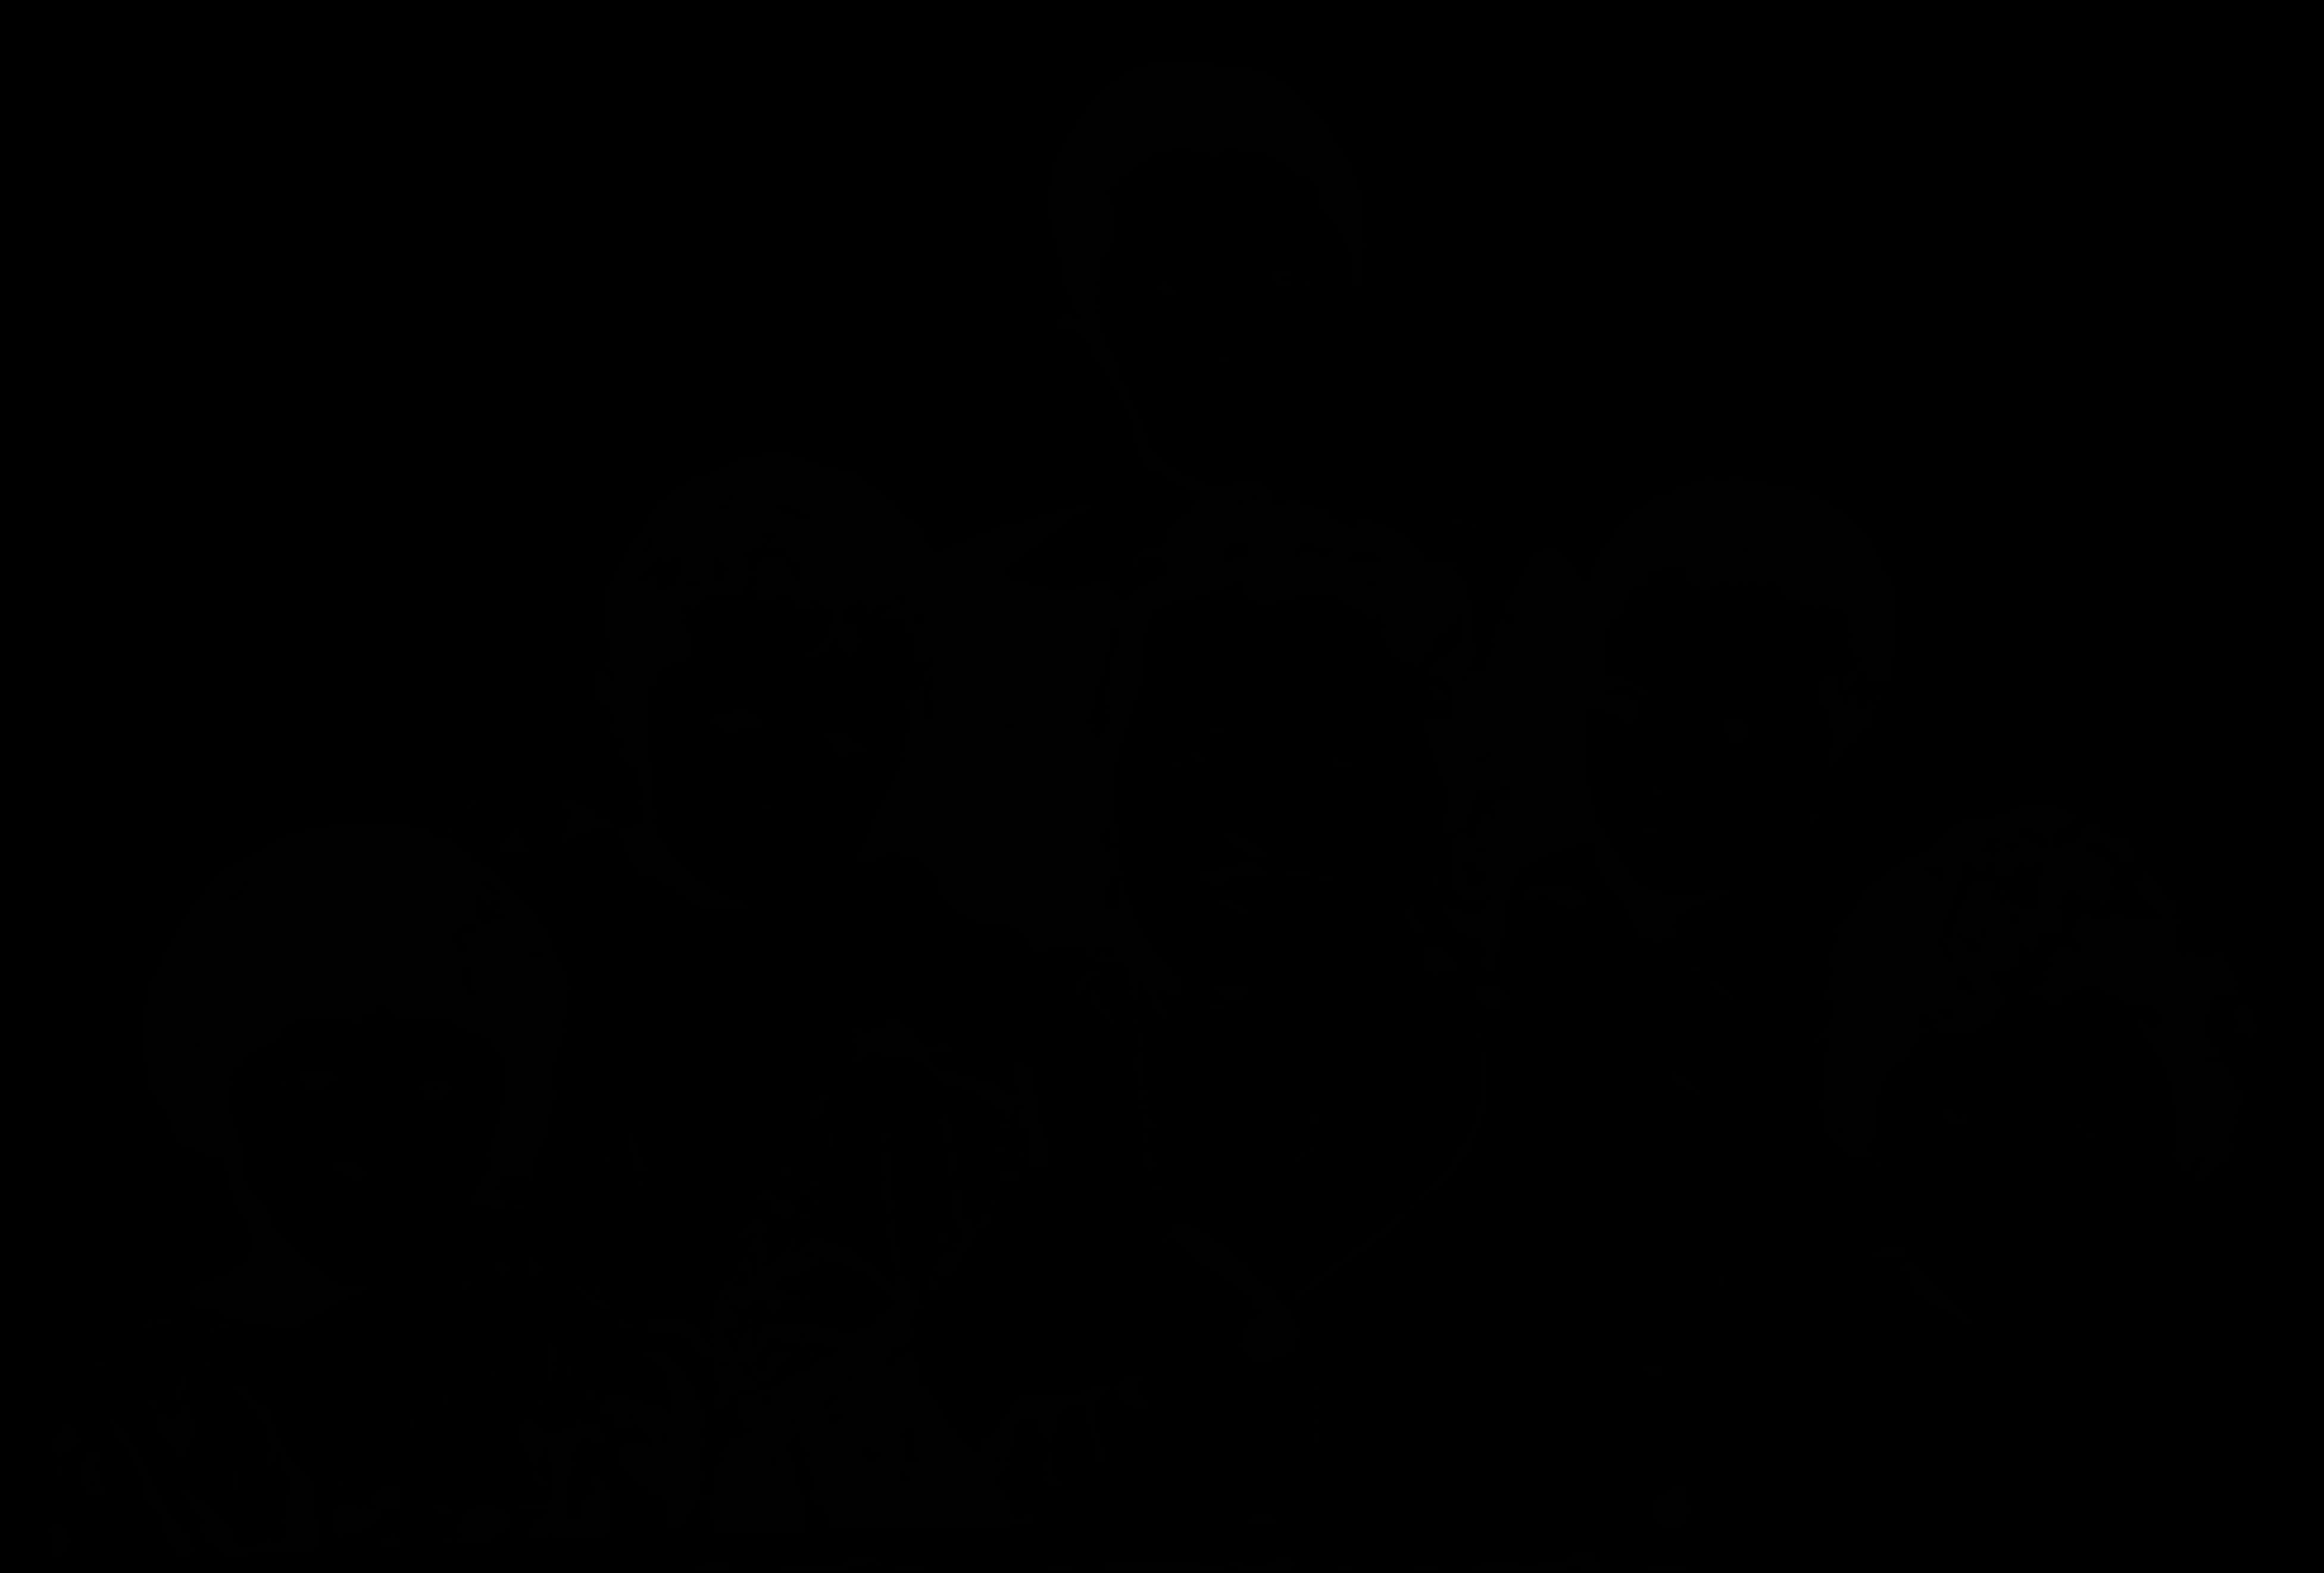
\includegraphics[width=0.3\linewidth]{2_S.jpg}
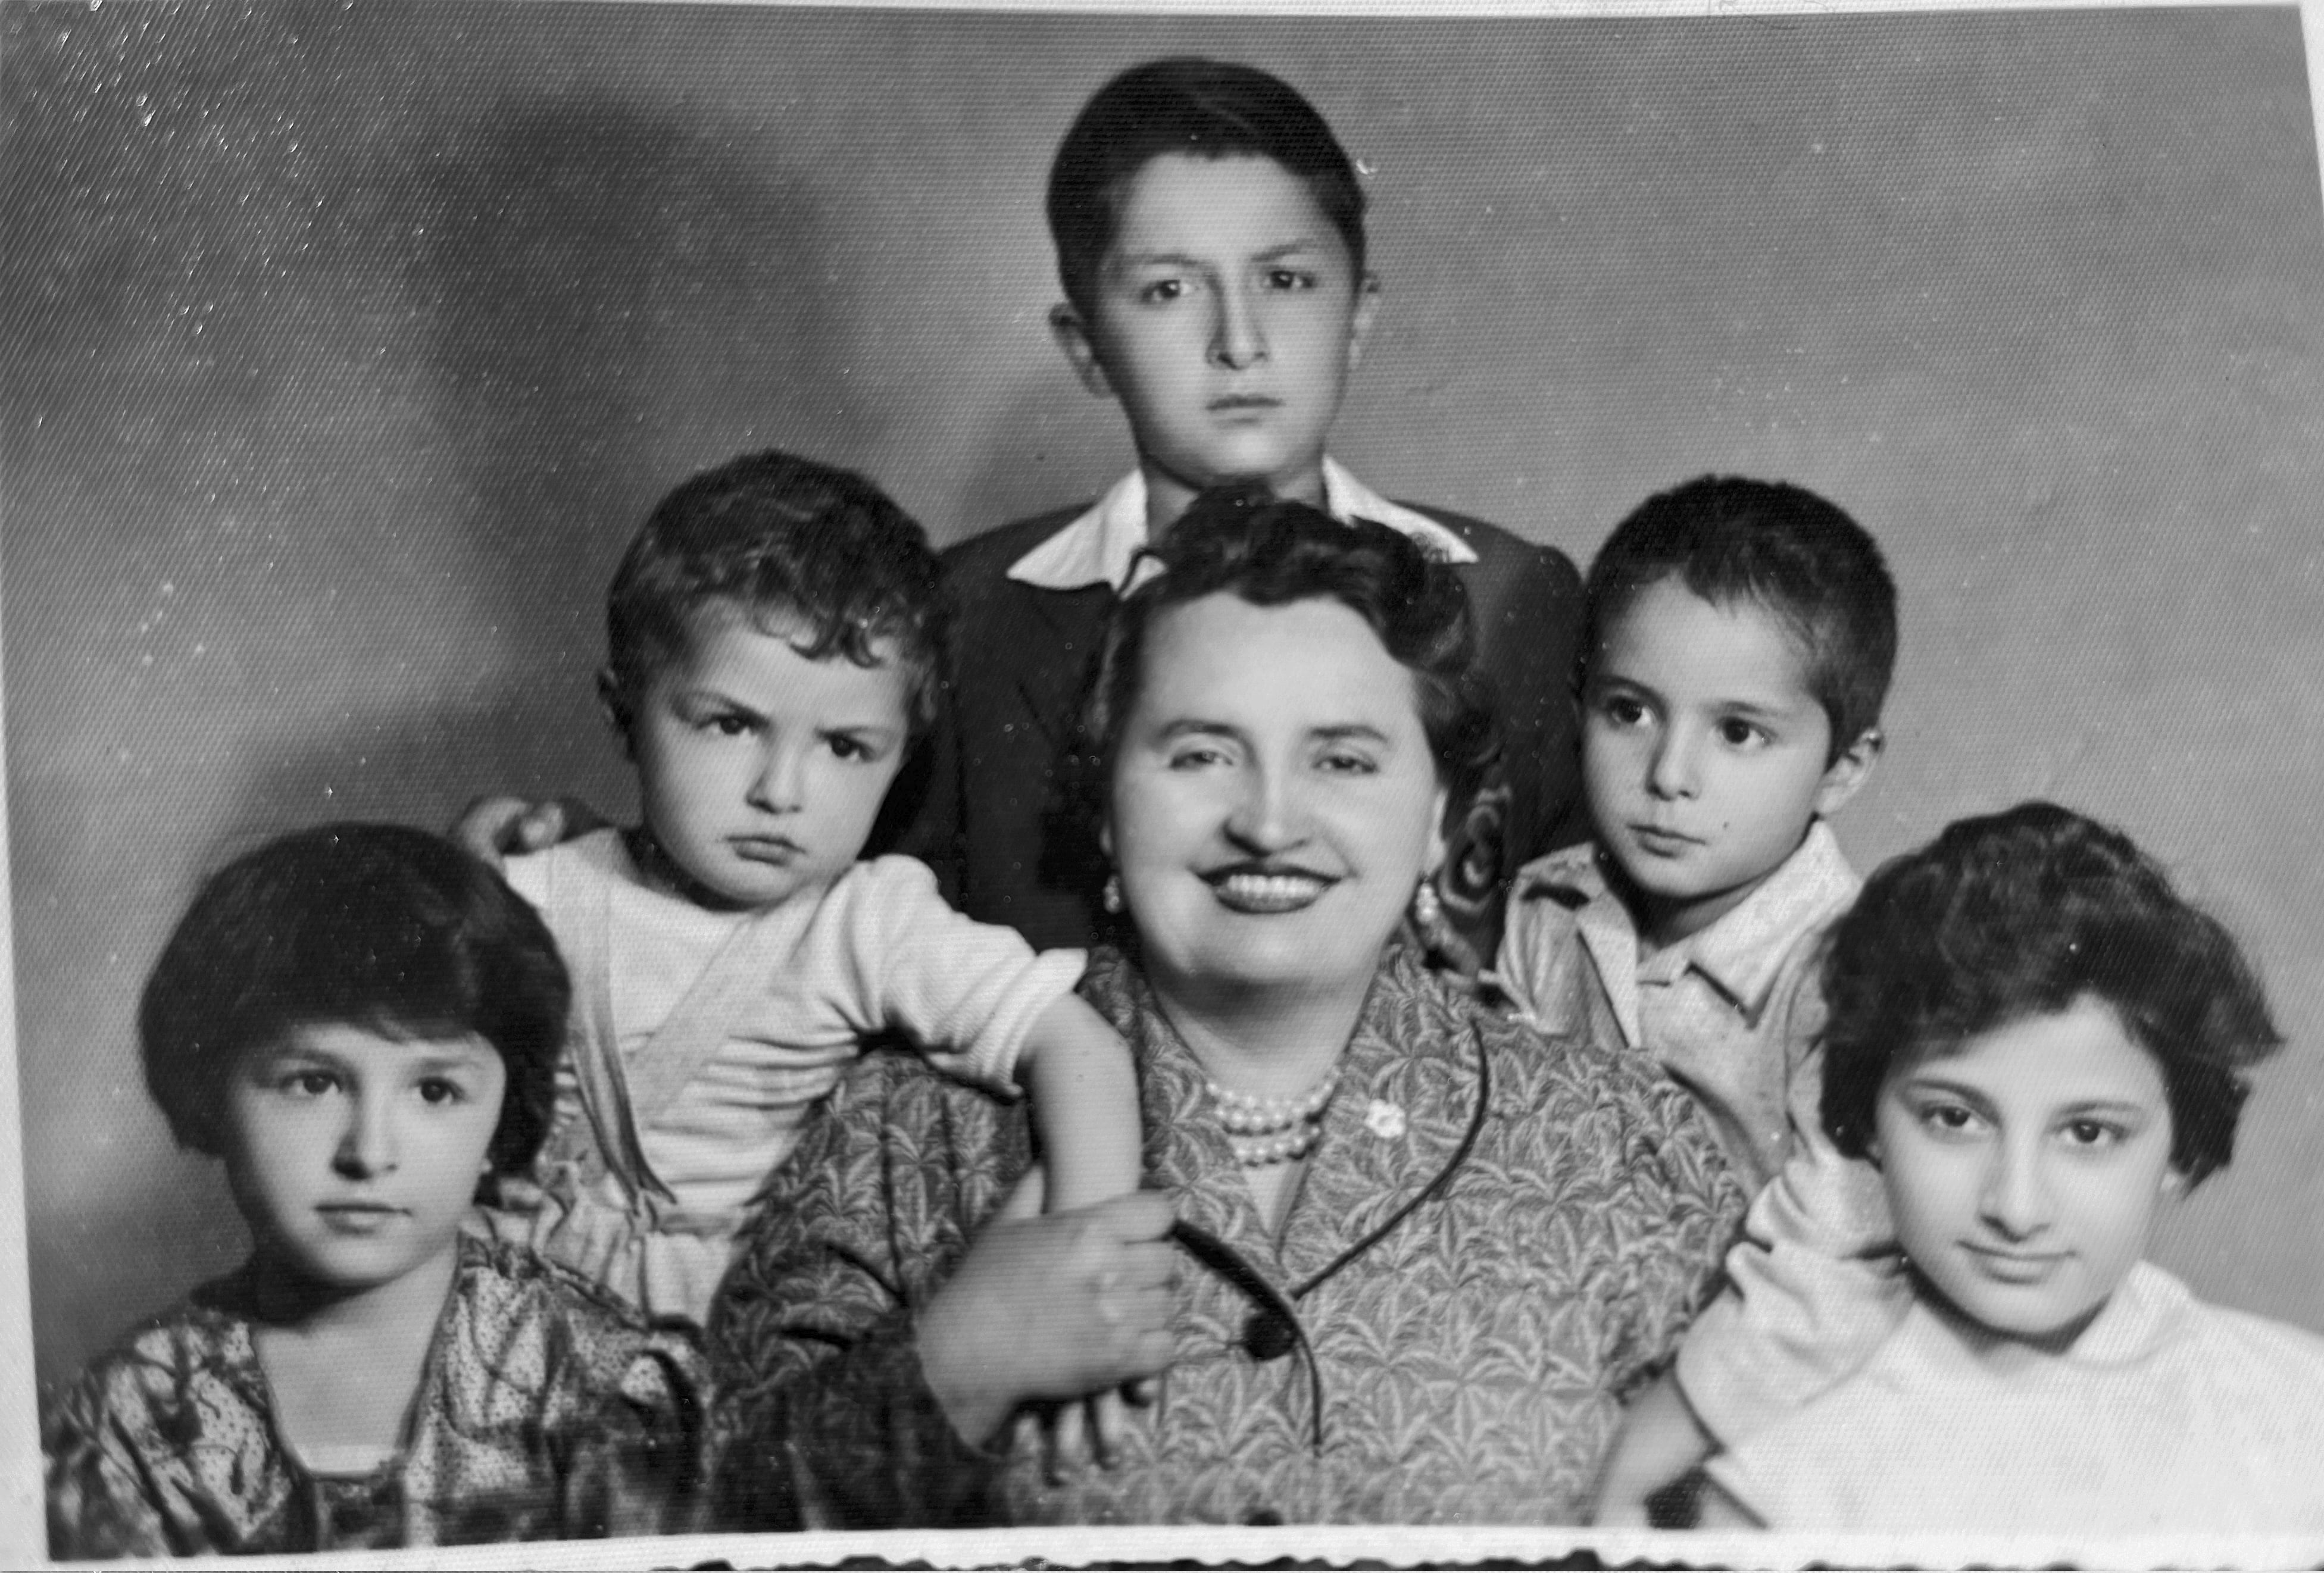
\includegraphics[width=0.3\linewidth]{2_I.jpg}
\newline
In the first image, we mostly observe colors close to yellow, and we got R and G channels which are brighter than the blue channel.\\
In the second image, we mostly observe colors close to red and purple, that's why we can see that R and B channels are brighter than the others.\\
Intensity channel is trivial as it is basically the average of R, G, and B channels. We can obtain gray scale image from this channel.
H channel of image1 is darker than the second. \\
One problem of the results is that we cannot observe S channel in both of the images. We investigated the problem, but ended up without a result.

\subsection{Step 6}
Edges detected with Laplacian Filter in image 1, with respect to RGB and HSI channels :\\
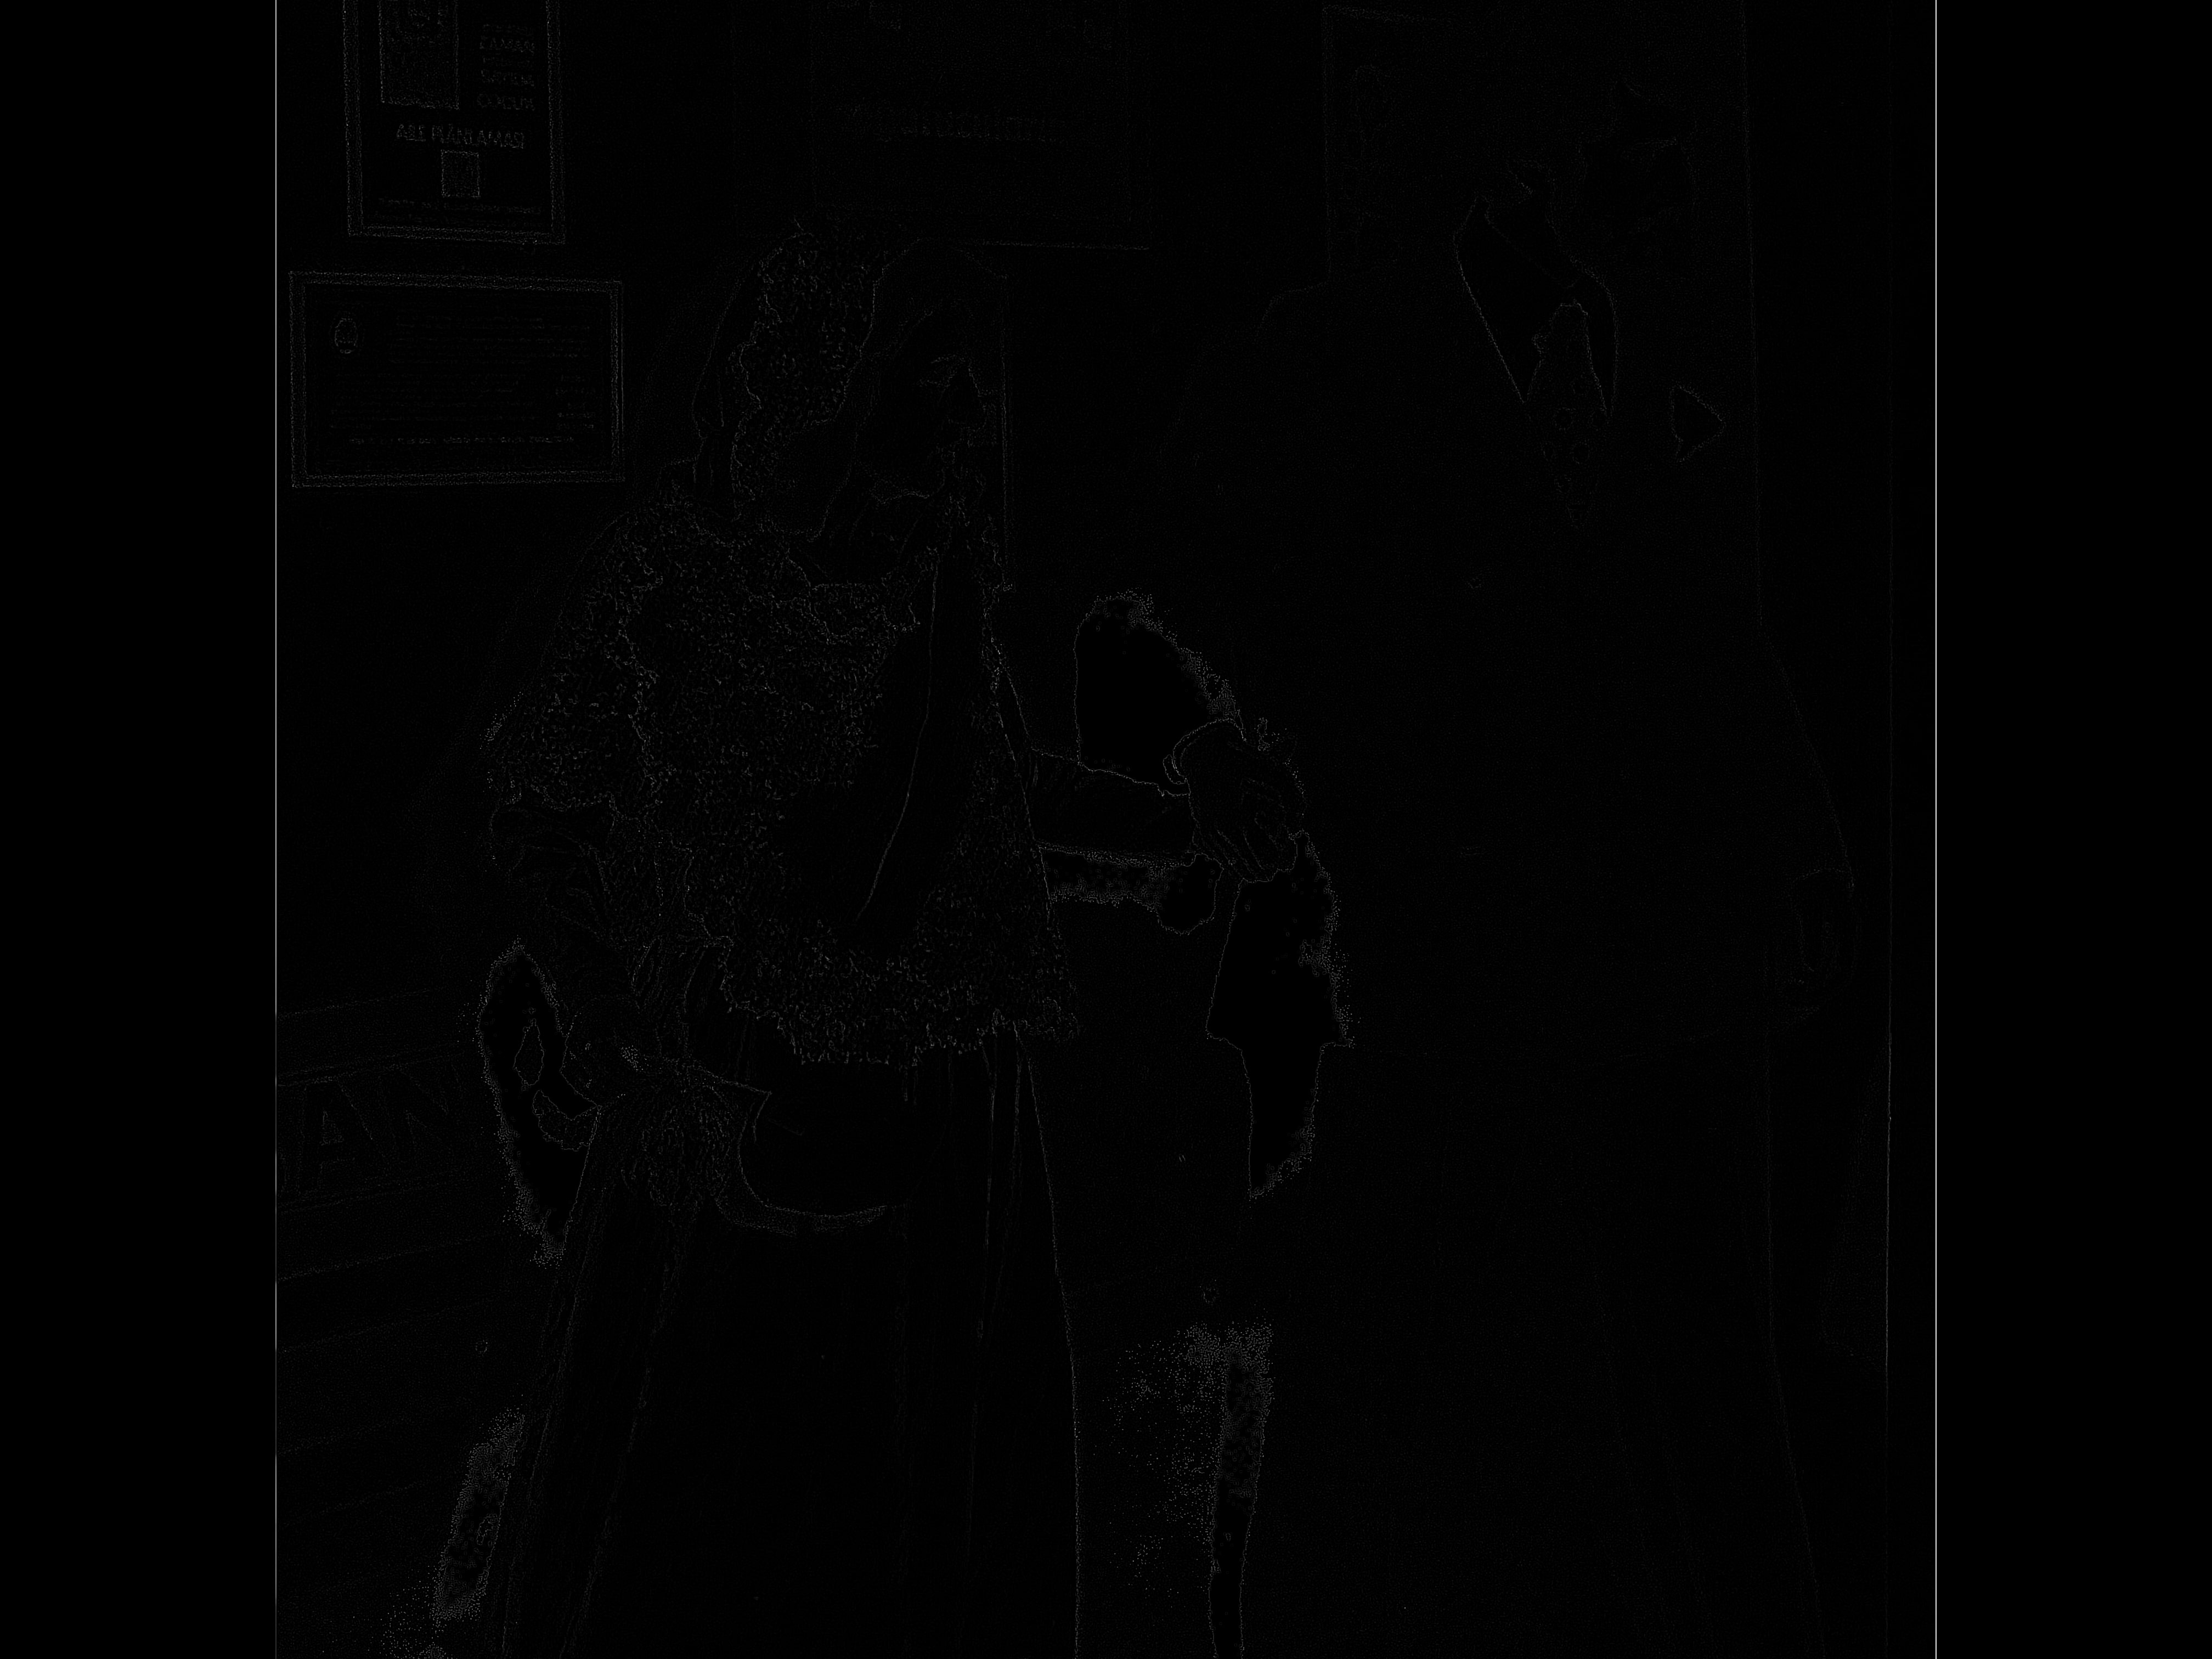
\includegraphics[width= 0.4\linewidth]{1_colored_edges_RGB.jpg}
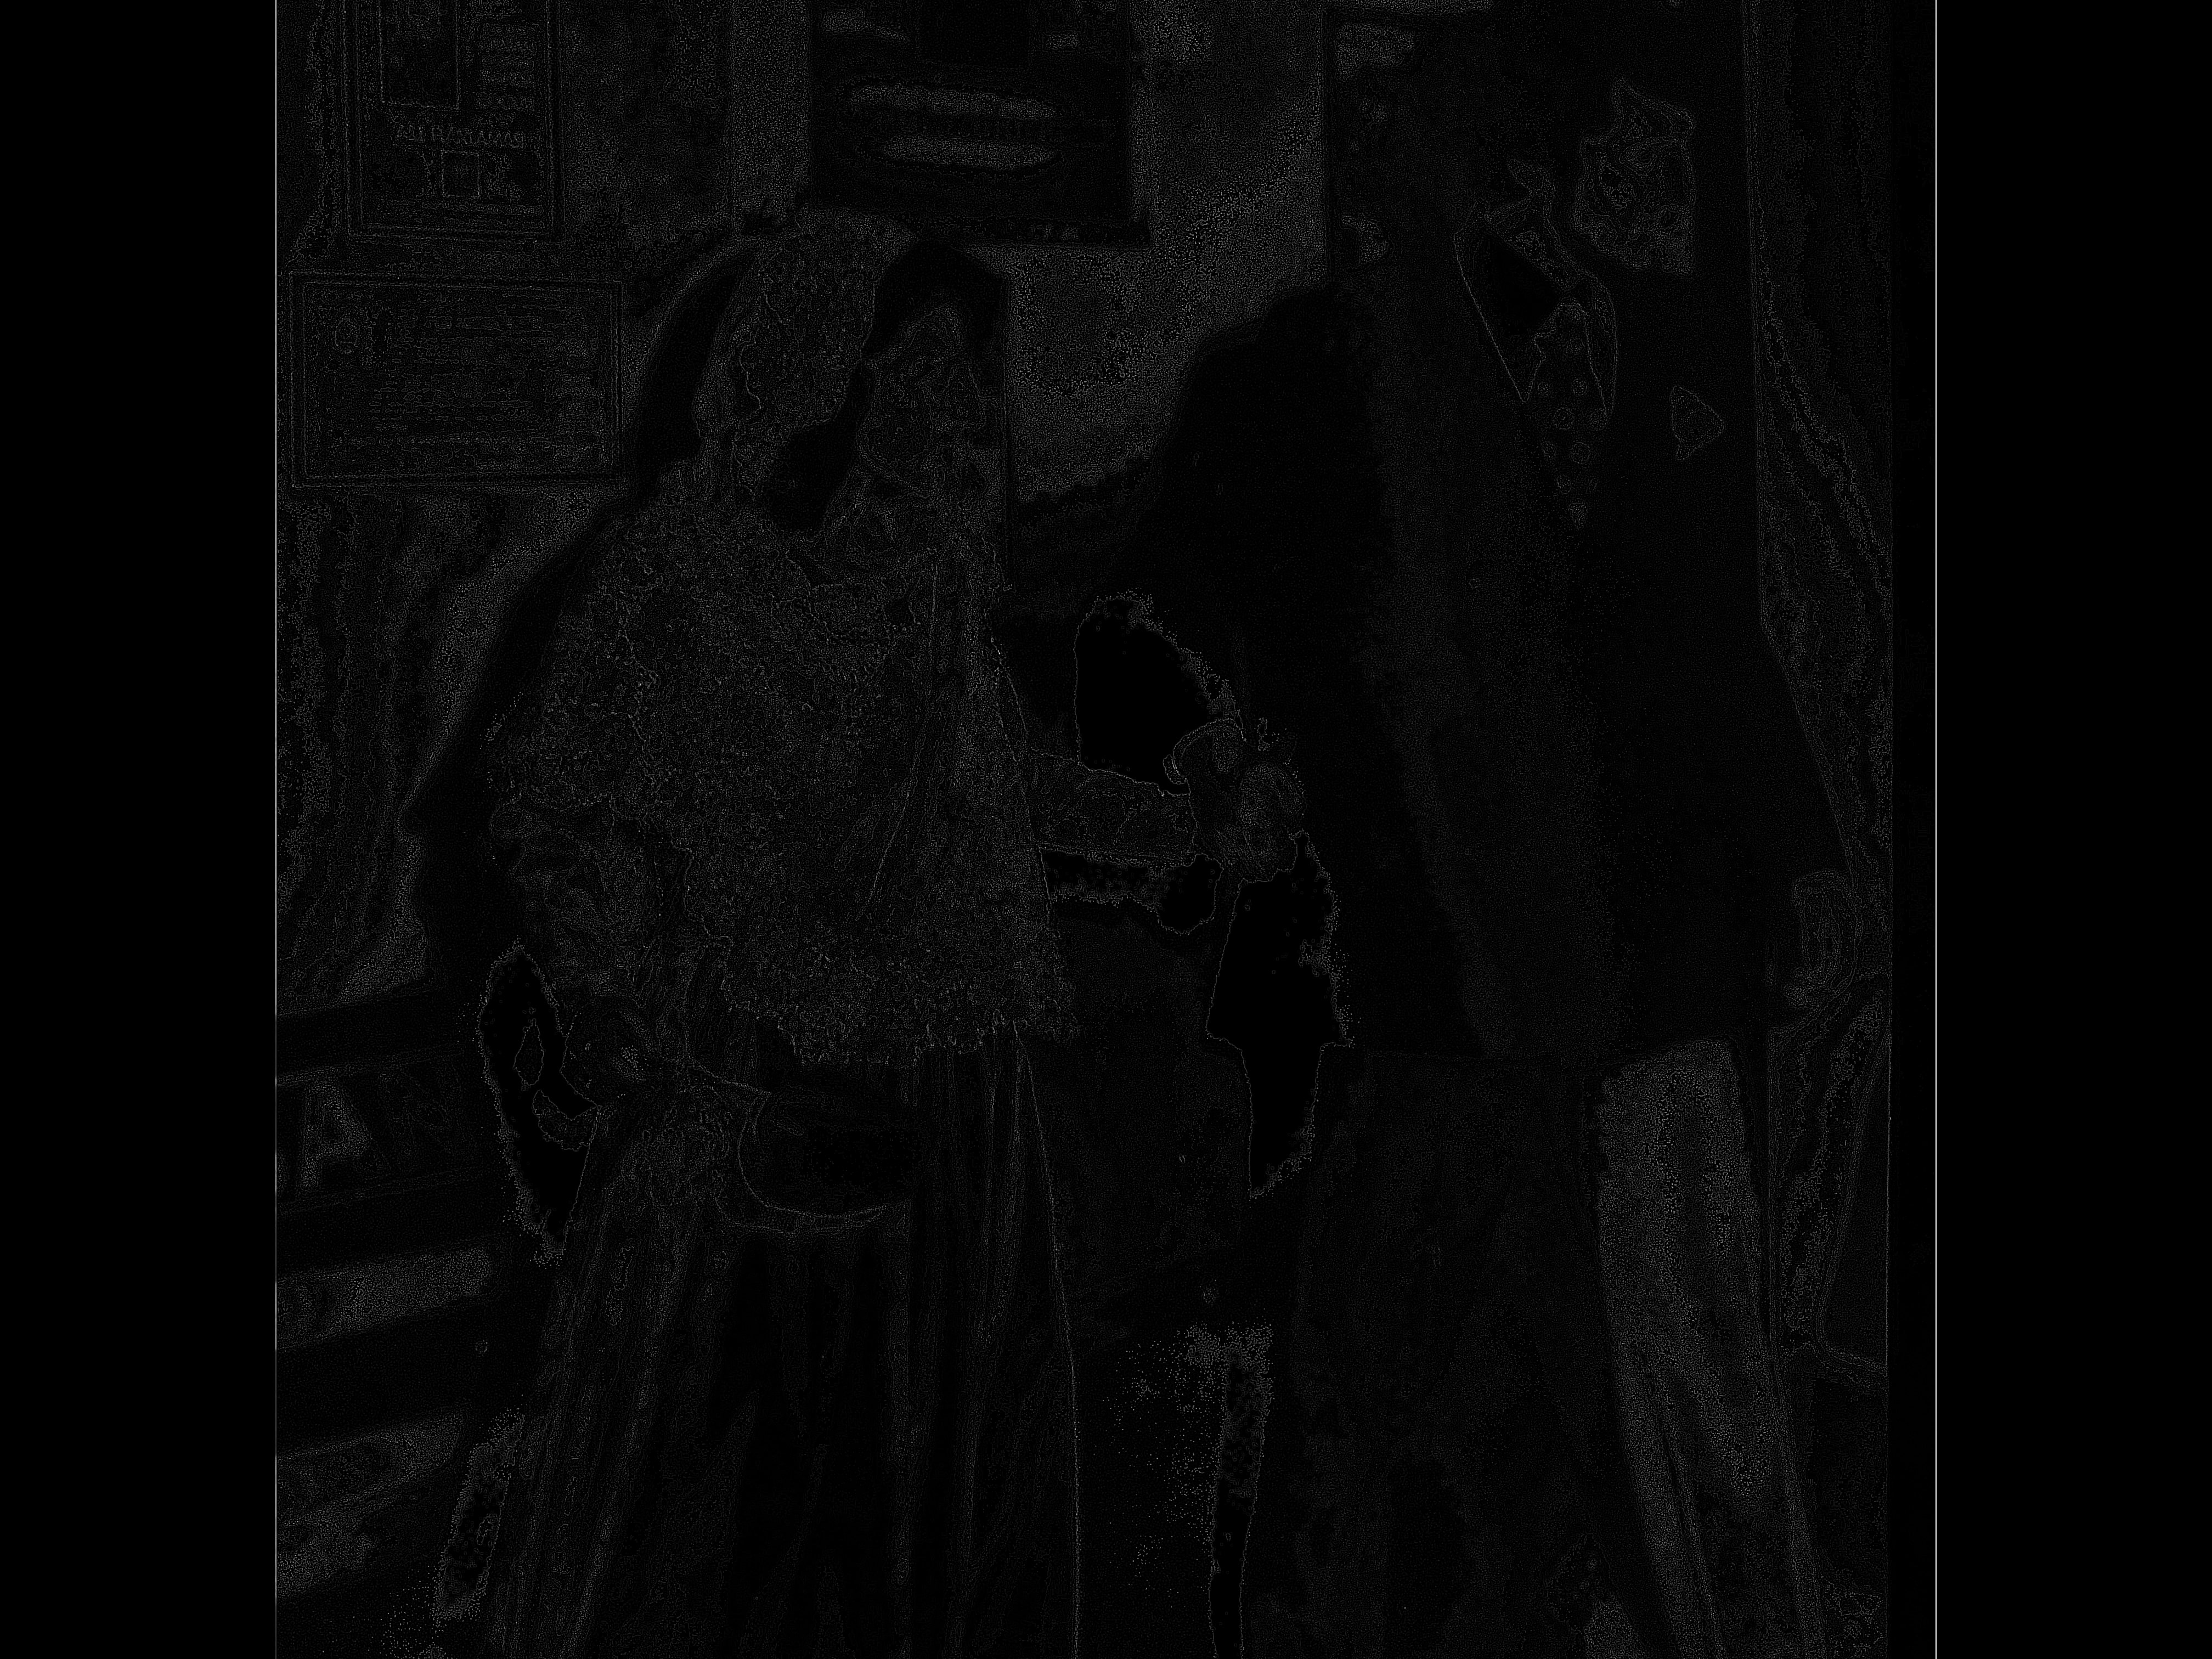
\includegraphics[width= 0.4\linewidth]{1_colored_edges_HSI.jpg}
\newline
Edges detected with Laplacian Filter in image 2, with respect to RGB and HSI channels :\\
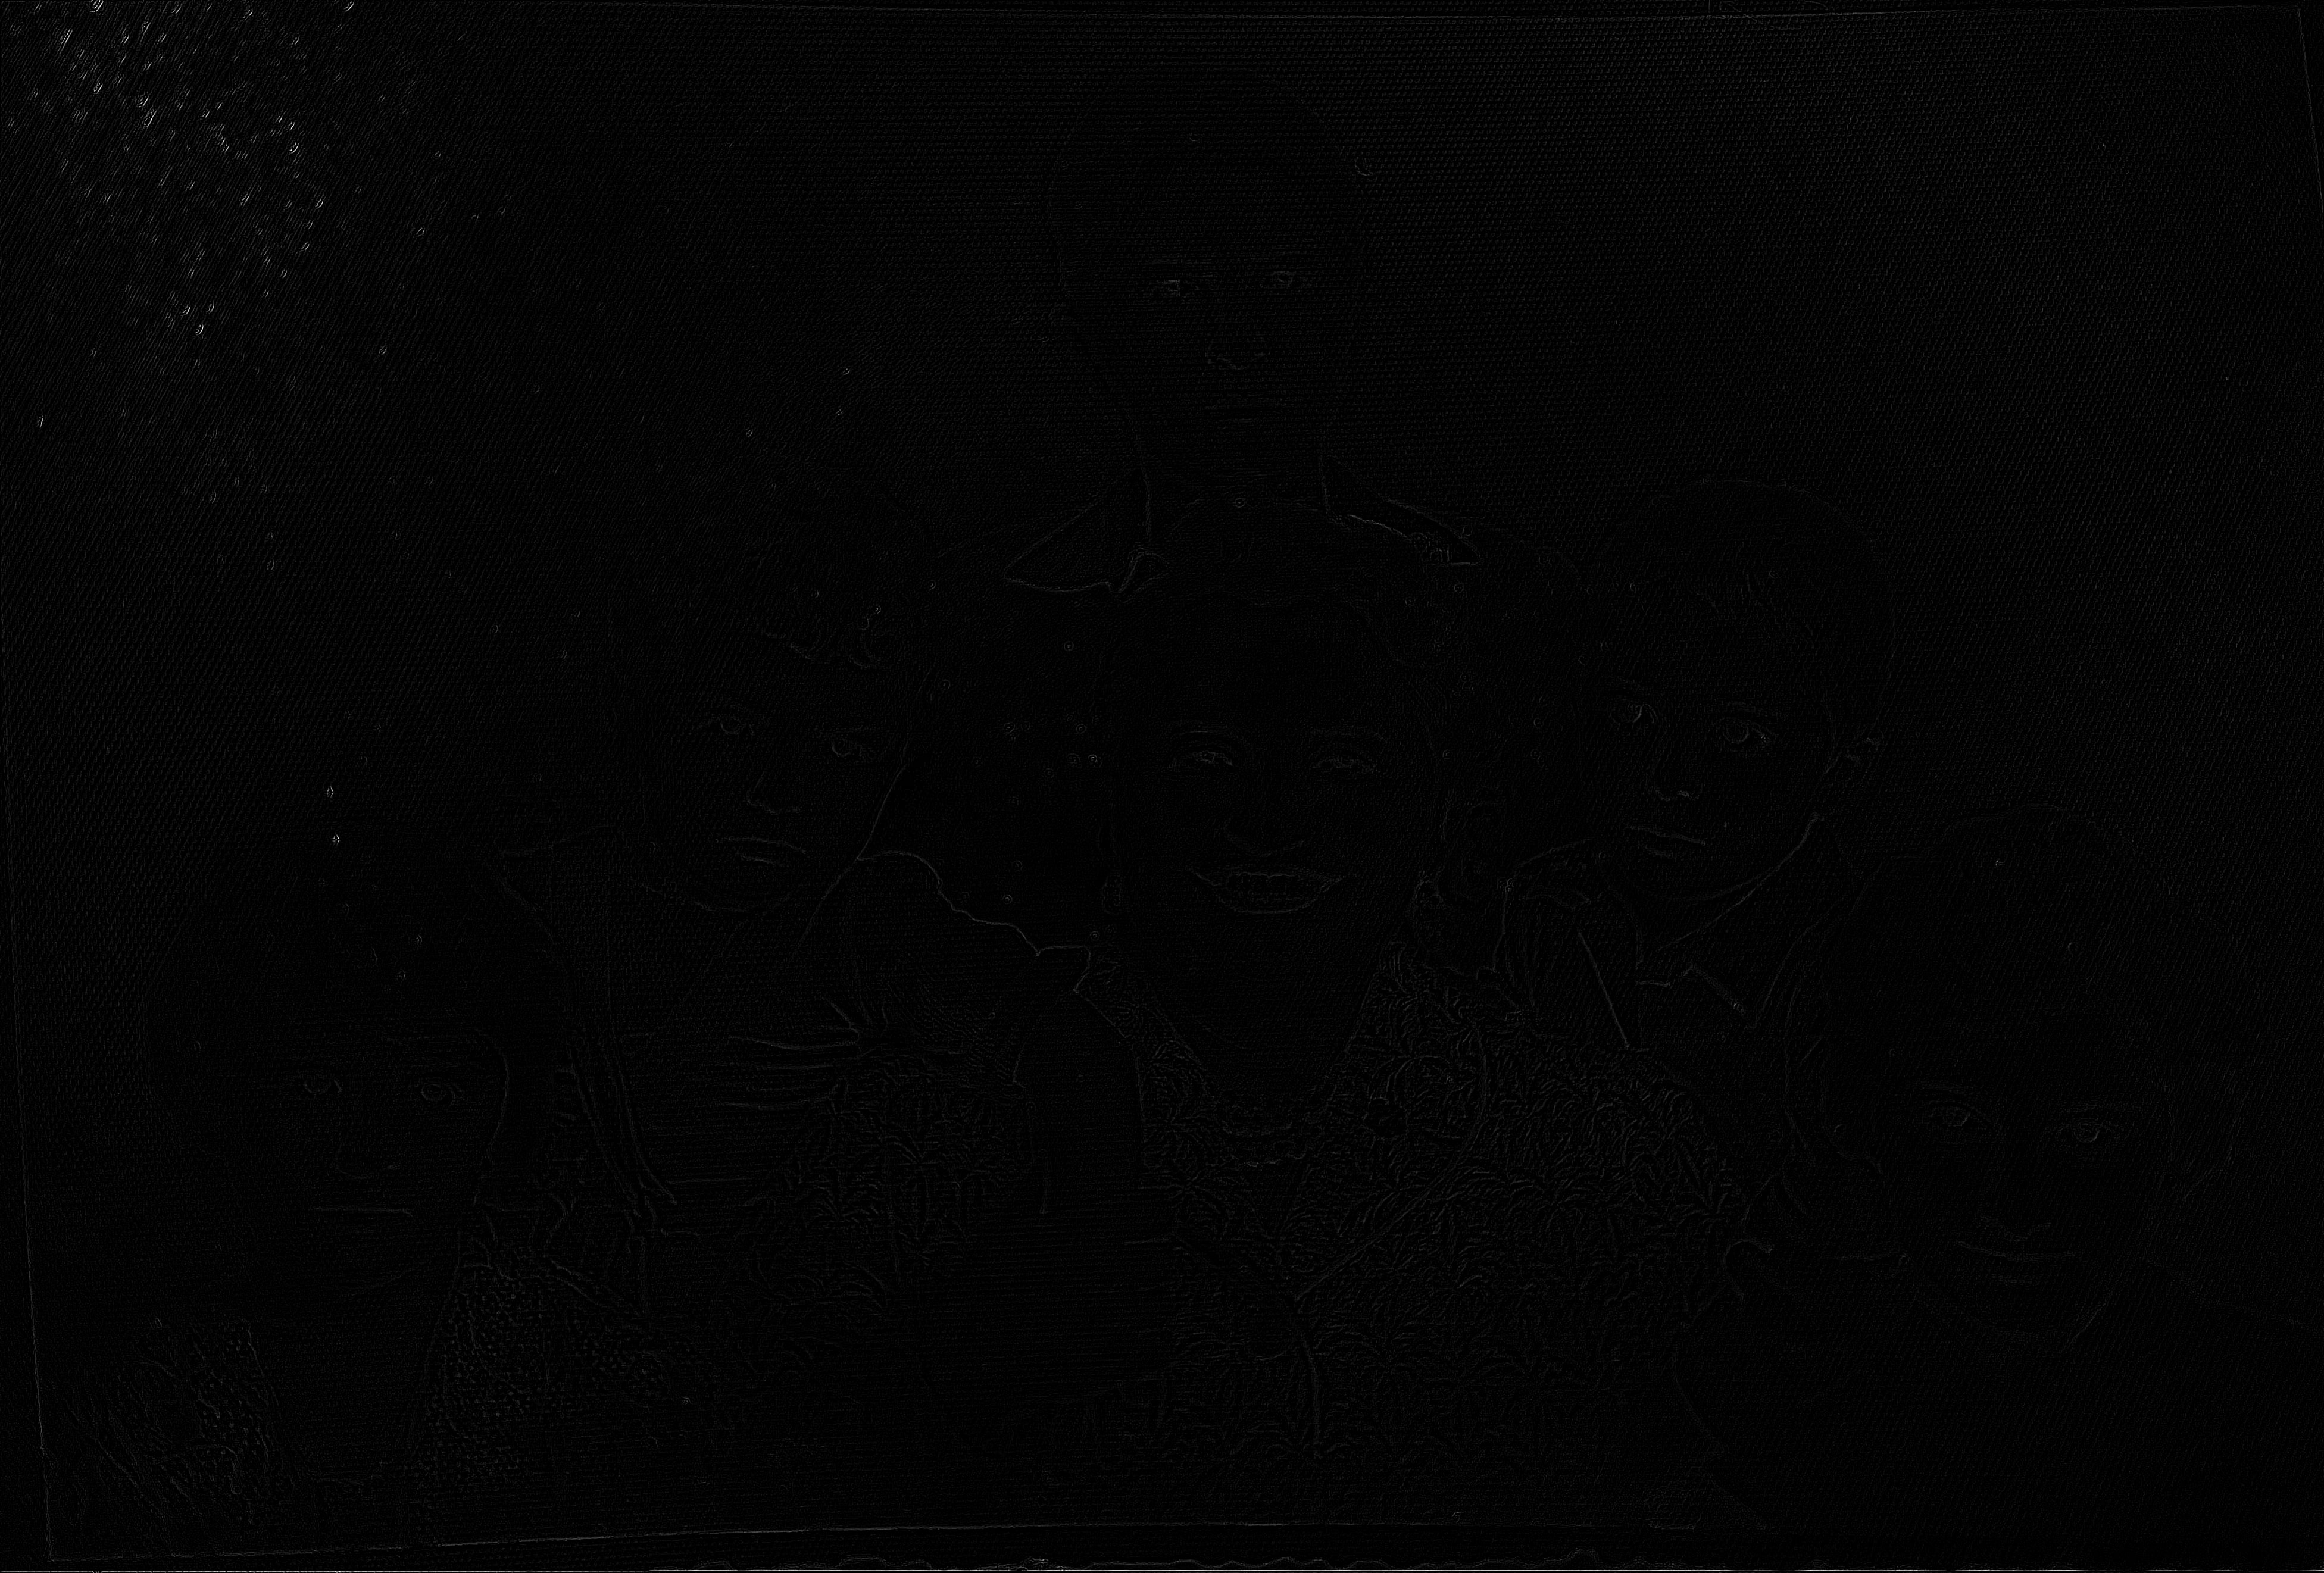
\includegraphics[width= 0.4\linewidth]{2_colored_edges_RGB.jpg}
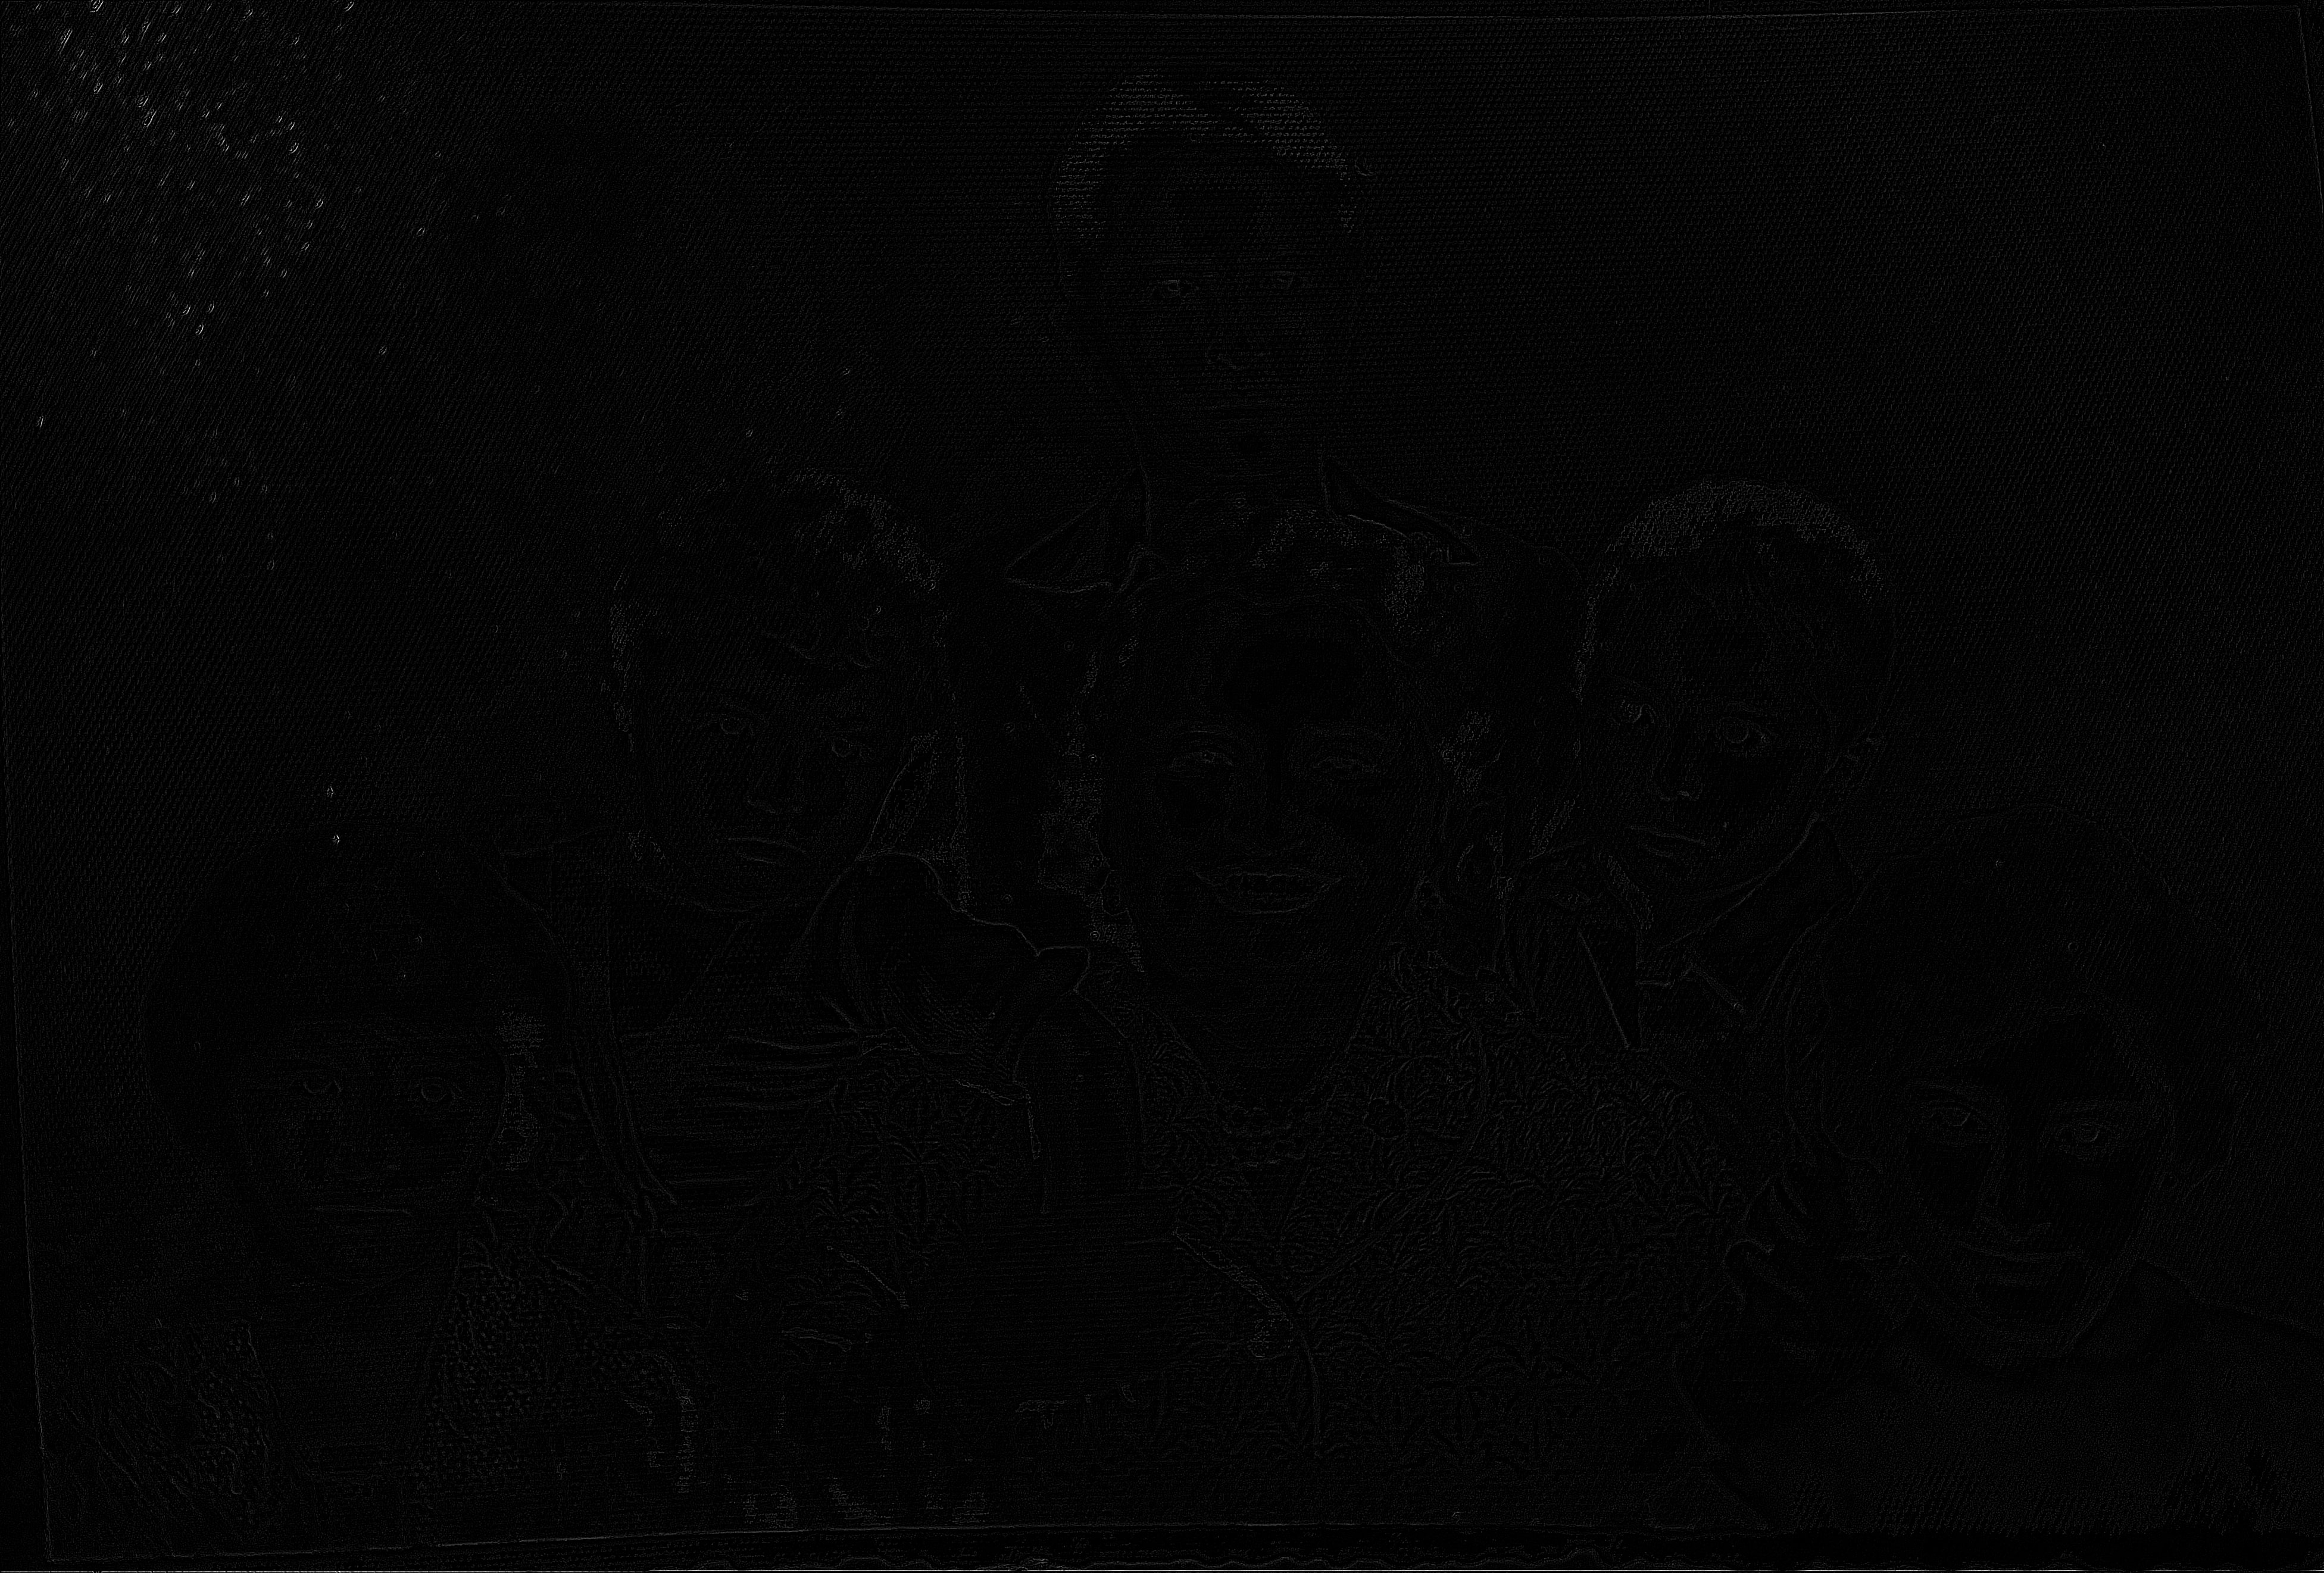
\includegraphics[width= 0.4\linewidth]{2_colored_edges_HSI.jpg}

In both images, we obtained better results when we use HSI image to detect the edges of the image.





\begin{thebibliography}{00}
\bibitem{b1} OpenCV documentation index. (n.d.). Retrieved November 5, 2022, from https://docs.opencv.org/ 
\bibitem{b2} Visualization with python. Matplotlib. (n.d.). Retrieved November 5, 2022, from https://matplotlib.org/ 
\bibitem{b3} J. A. Stark, "Adaptive image contrast enhancement using generalizations of histogram equalization," in IEEE Transactions on Image Processing, vol. 9, no. 5, pp. 889-896, May 2000, doi: 10.1109/83.841534.
\end{thebibliography}

\end{document}
